\documentclass[12pt,twoside]{book}

\usepackage[hcentering,twoside,a4paper,outer=1.4in,inner=0.8in,vmargin=3cm]{geometry}

\newif\ifanimate
\animatefalse

\usepackage[utf8]{inputenc}
\ifanimate
\usepackage{animate}
\fi
\usepackage{verbatim}
\usepackage{fancyhdr}
\usepackage{flipbook}
\usepackage{wrapfig}
\usepackage{afterpage}
\usepackage{pdflscape}
\usepackage{natbib}
\usepackage{graphicx}
\usepackage{amsthm}
\usepackage{amsmath}
\usepackage{setspace}
\usepackage{lmodern}
\usepackage{float}
\usepackage{textcomp}
\usepackage{floatflt}
\usepackage{listings}
%\usepackage{ulem}
\usepackage{color}
\usepackage{tabularx}
\usepackage{multirow}
\usepackage{bbold}
\usepackage{subfigure}
\usepackage{pdfpages}


\setlength{\headheight}{15pt}

\lstset{
  language=Python,
  showstringspaces=false,
  formfeed=\newpage,
  tabsize=4,
	breaklines=true,
	breakautoindent=true,
  commentstyle=\itshape,
  basicstyle=\ttfamily,
  morekeywords={models, lambda, forms},
  keywordstyle=\color[rgb]{0,0,1},
  commentstyle=\color[rgb]{0.133,0.545,0.133},
  stringstyle=\color[rgb]{0.627,0.126,0.941}
}
\restylefloat{table}

\usepackage{sidecap}
\usepackage[scaled]{helvet}
\usepackage{caption}

\setlength{\headheight}{28pt}
%\setlength{\marginparwidth}{1in}

\newcounter{todos}
\newcounter{comments}
\newcounter{figcomments}
\newcounter{advisorcomments}
\newcounter{questions}

\setcounter{tocdepth}{3}

\definecolor{grey}{rgb}{0.4,0.4,0.4}
\definecolor{red}{rgb}{1.0,0,0}
\definecolor{brown}{rgb}{0.5,0.0,0.0}
\definecolor{orange}{rgb}{0.7,0.3,0.}
\DeclareCaptionFont{grey}{\color{grey}}
\captionsetup{margin=10pt,font=small,labelfont=bf,format=plain,textfont=grey,labelfont=grey}

\renewcommand*\familydefault{\sfdefault} %% Only if the base font of the document is to be sans serif
\usepackage[T1]{fontenc}
\linespread{1.2}

\title{\normalsize Thèse de Doctorat de l'Université Pierre et Marie Curie \\ Specialité: Physique de la matière condensée \\ Ecole Doctorale de Physique de la Région Parisienne - ED 107 \bigskip \\ \huge Demonstrating Quantum Speed-Up with a Two-Transmon Quantum Processor}
\author{Présentée par \bigskip \\ \bigskip \huge Andreas Dewes \\ \small Pour obtenir le grade de ``Docteur de l'Université Pierre et Marie Curie'' \vspace{3cm} \\ Soutenue le 15 novembre 2012 devant le jury composé de: \\ Prof. Alexey Ustinov (rapporteur) \\ Dr. Olivier Buisson (rapporteur) \\ Prof. Jean-Michel Raimond \\ Prof. David DiVincenzo \\ Dr. Denis Vion}
\date{\vspace{2cm} Thèse préparée au sein du Service de Physique de l'Etat Condensé, CEA Saclay}
\theoremstyle{definition}
\newtheorem{theorem}{Theorem}[chapter]
\newtheorem{axiom}{Axiom}[theorem]

\newcommand{\LA}[1]{\begin{mathcal}L\end{mathcal}_{#1}} % for Dirac brackets
\newcommand{\Or}{\begin{mathcal}C\end{mathcal}} % for Dirac brackets
\newcommand{\De}{\begin{mathcal}D\end{mathcal}} % for Dirac brackets
\newcommand{\Er}{\begin{mathcal}E\end{mathcal}} % for Dirac brackets
\newcommand{\bracket}[1]{\left< #1 \right>} % for Dirac brackets
\newcommand{\ket}[1]{\left| #1 \right>} % for Dirac bras
\newcommand{\bra}[1]{\left< #1 \right|} % for Dirac kets
\newcommand{\mcal}[1]{\begin{mathcal}#1\end{mathcal}}

\newcommand{\todo}[1]{
  \addtocounter{todos}{1}
	\textcolor{red}{!\arabic{todos}!}
	\marginpar{
		\begin{spacing}{0.5}
			\textcolor{red}
				{
				{\flushleft \scriptsize  \linespread{0.8} To Do \arabic{todos}: #1}
				}
		\end{spacing}
	}
}

\renewcommand{\todo}[1]{}

\newcommand{\figcomment}[1]{
	%To do: Fix the bug that makes the counter value increase by 2 each time this command is called.
	\addtocounter{figcomments}{1}
	\textcolor{orange}{Figure Comment \arabic{figcomments}: #1}
}

\renewcommand{\comment}[1]{
  \addtocounter{comments}{1}
	\textcolor{orange}{!\arabic{comments}!}
	\marginpar{
		\begin{spacing}{0.5}
			\textcolor{orange}
				{
				{\flushleft \scriptsize  \linespread{0.8} Comment \arabic{comments}: #1}
				}
		\end{spacing}
	}
}

\newcommand{\question}[1]{
  \addtocounter{questions}{1}
	\textcolor{blue}{?\arabic{questions}?}
	\marginpar{
		\begin{spacing}{0.5}
			\textcolor{blue}
				{
				{\flushleft \scriptsize  \linespread{0.8} Question \arabic{questions}: #1}
				}
		\end{spacing}
	}
}

\newcommand{\advisorcomment}[1]{
  \addtocounter{advisorcomments}{1}
	\textcolor{yellow}{!\arabic{advisorcomments}!}
	\marginpar{
		\begin{spacing}{0.5}
			\textcolor{yellow}
				{
				{\flushleft \scriptsize  \linespread{0.8} Advisor comment \arabic{advisorcomments}: #1}
				}
		\end{spacing}
	}
}

\fancyhead[OL]{Andreas Dewes}

\cfoot{}
\rfoot[\thepage]{\thepage}

\begin{document}

\pagestyle{plain}
\pagenumbering{gobble}


\ifanimate
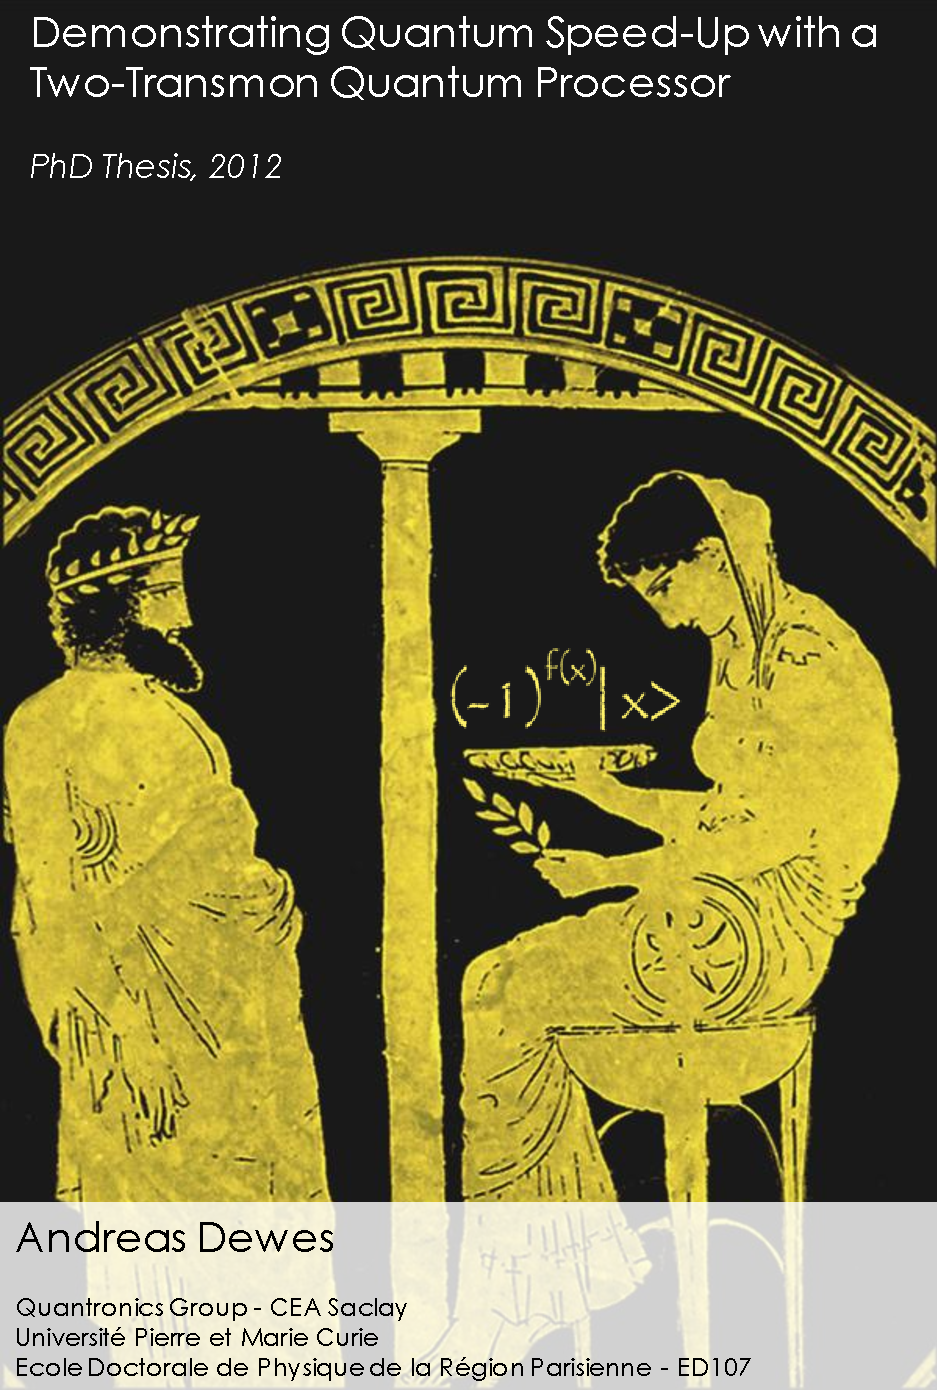
\includepdf[pages={1},fitpaper=true]{cover_web.pdf}
\else
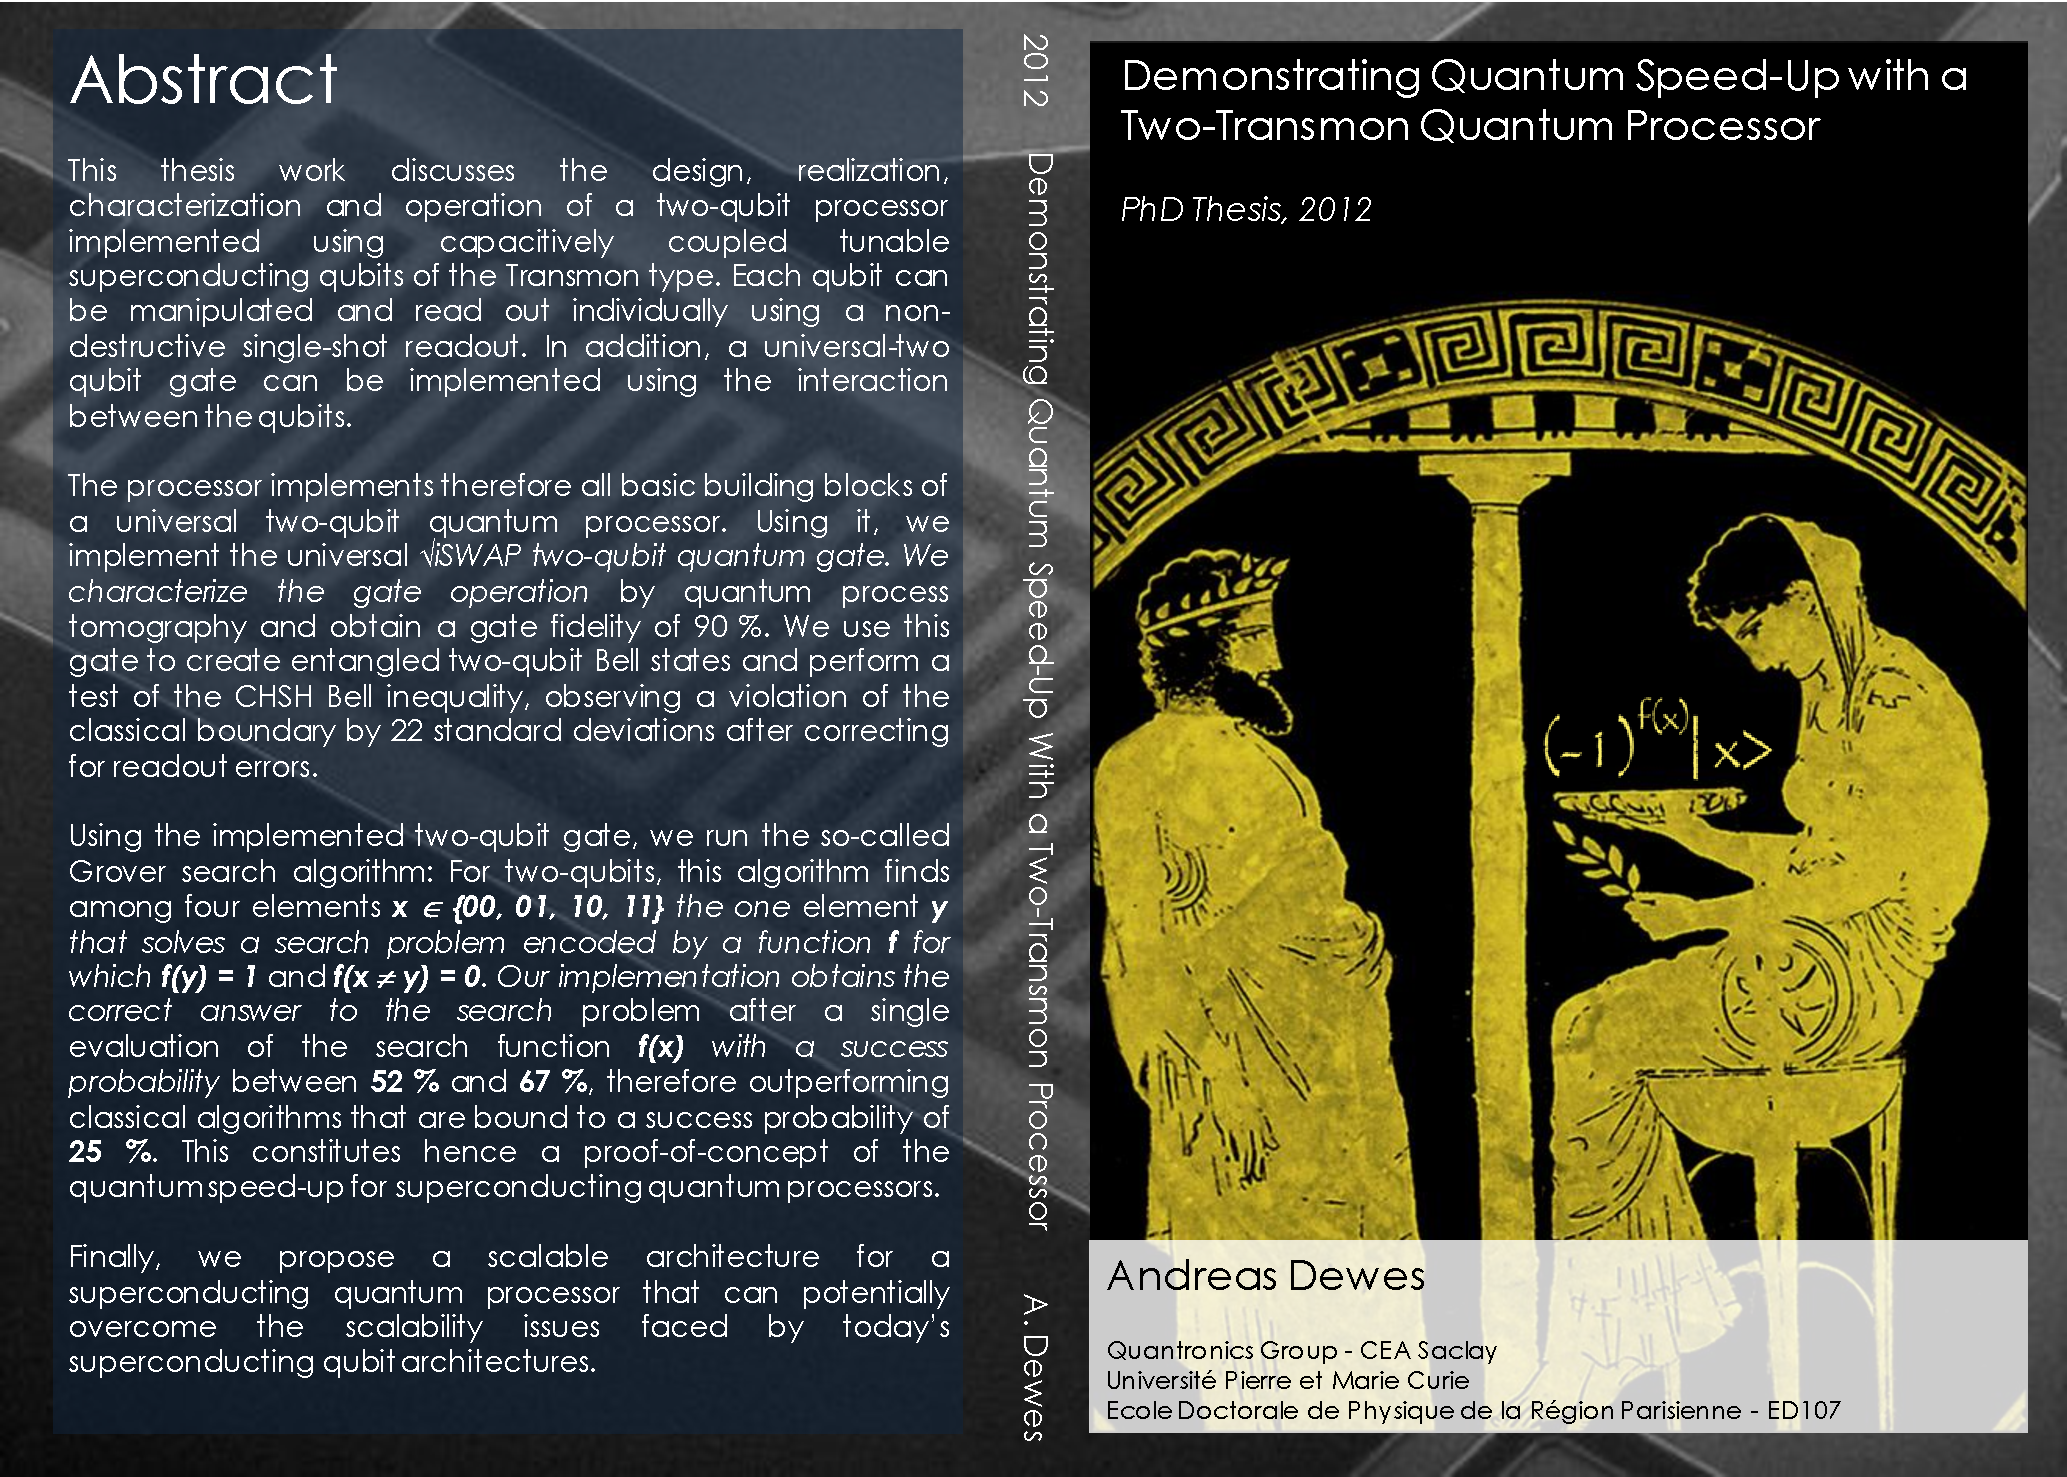
\includepdf[pages={1},fitpaper=true]{cover.pdf}
\fi

\maketitle

\thispagestyle{empty}

{\small
\textbf{Cover Illustration}: King Aegeus asking the priestess Pythia, the Oracle of Delphi, for advice concerning family matters. Analogously, in this work we make use of a quantum Oracle to find the solution to a mathematical problem faster than possible when using classical computing\footnote{Incidentally, we use a language called Python to convey the messages of our Oracle.}. Similar to the prophecies uttered by the ancient Oracle, the solutions that we obtain also tend to be slightly ambiguous.}


\chapter*{Acknowledgments}

This thesis would not exist without the invaluable help of my colleagues at the CEA Saclay. Special thanks go to my advisers \textbf{Denis Vion}, \textbf{Patrice Bertet} and \textbf{Daniel Esteve}: Countless times they provided me with scientific and personal advice and were always patient, optimistic and supportive, even at times when I was not.

\smallskip

In addition, I thank \textbf{Florian Ong}, who worked as a Post-Doc in the group during the first year of my thesis and fabricated the original qubit chip with which most of the measurements discussed in this thesis have been made. Also, I want to thank \textbf{Agustin Palacios-Laloy}, who introduced me to his setup and helped me to get started with my measurements. Furthermore, I want to thank \textbf{Nicolas Boulant}, who, with his experience in quantum state \& process tomography, helped me to understand the data of the iSWAP experiment.

\smallskip

Last but not least, I want to thank all of my colleagues for their help and support, as well as for the countless interesting discussions I had with them. They made the Quantronics lab a very special and enjoyable place to work at.

%\listoffigures

%\listoftables

\chapter*{Short Summary}

\begin{center}
{\huge Demonstrating Quantum Speed-Up with a Two-Transmon Quantum Processor} \\ \bigskip
\end{center}

The thesis work discusses the design, realization, characterization and operation of a two-qubit processor implemented using capacitively coupled tunable superconducting qubits of the Transmon type. Each qubit can be manipulated and read out individually using a non-destructive single-shot readout. In addition, a universal-two qubit gate can be implemented using the interaction between the qubits. The processor implements therefore all basic building blocks of a universal two-qubit quantum processor. Using it, we implement the universal $\sqrt{i\mathrm{SWAP}}$ two-qubit gate, characterizing the gate operation by quantum process tomography and obtaining a gate fidelity of 90 \%. We use this gate to create entangled two-qubit Bell states and perform a test of the CHSH Bell inequality, observing a violation of the classical boundary by 22 standard deviations after correcting for readout errors. 

\smallskip

Using the implemented two-qubit gate, we run the so-called Grover search algorithm: For two-qubits, this algorithm finds among four elements $x \in \{00,01,10,11\}$ the one element $y$ that solves a search problem encoded by a function $f$ for which $f(y)=1$ and $f(x\ne y)=0$. Our implementation retrieves the correct answer to the search problem after a single evaluation of the search function $f(x)$, with a success probability between 52 \% and 67 \%, therefore outperforming classical algorithms that are bound to a success probability of 25 \%. This constitutes therefore a proof-of-concept of the quantum speed-up for superconducting quantum processors.

\smallskip

Finally, we propose a scalable architecture for a superconducting quantum processor that can potentially overcome the scalability issues faced by today’s superconducting qubit architectures.

\tableofcontents

\newpage

\rhead[]{
\setlength\unitlength{1cm}
\begin{picture}(0,0)
\put(-0.2,-0.36){
\fbImageF{"./data/ct5/film of swap/matrices/matrix_"}{pdf}{scale=0.18}
}
\end{picture}
}

\chapter{Introduction \& Summary}

%Provide a short summary of the whole PhD thesis:
% -Introduction to QC & CQED
% -Building Blocks of Superconducting Quantum Processors
% -Realization of a Two-Transmon QP
% -Tune-Up & Characterization of the Universal Two-Qubit Gate
% -Grover's Algorithm: Introduction & Background
% -Implementation on the Two-Qubit Processor
% -Design of a Scalable QC Architecture

\section{Quantum Computing \& Circuit Quantum Electrodynamics}

\begin{figure}
	\centering
		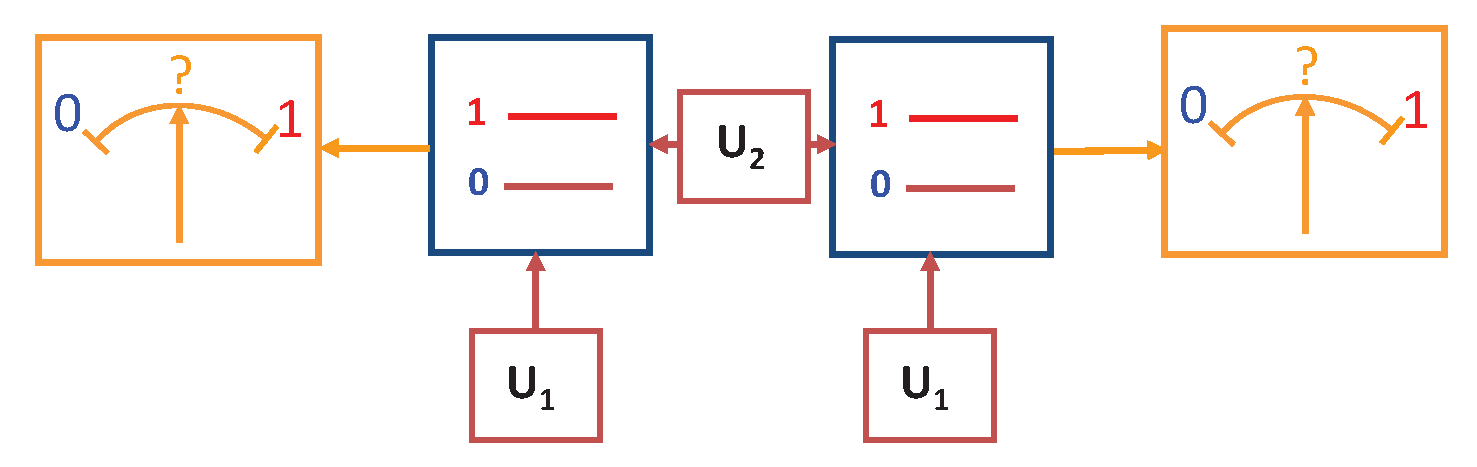
\includegraphics[width=0.8\textwidth]{./material/papers/grover/submission1/Fig1}
	\caption[Blueprint of a two-qubit quantum processor]{The blueprint of a two-qubit quantum processor. Shown are two qubits that can be individually manipulated ($U_1$) and are connected by a universal two-qubit gate $U_2$. Each of the qubits can be read out individually.}
	\label{fig:qubit_processor_blueprint}
\end{figure}

This thesis presents experiments performed with a superconducting two-qubit quantum processor. The main goal of this work was to demonstrate a possible quantum computing architecture using superconducting qubits that follows the canonical blueprint of a quantum processor as shown in fig. \ref{fig:qubit_processor_blueprint}, following the four criteria formulated by \cite{divincenzo_physical_2000}. Following this definition, a universal quantum computer is a register of quantum bits -- or qubits -- on which one can perform universal single- and two-qubit quantum gates, read out the state of each qubit individually and with high fidelity and reset the qubit register to a well-defined state.

Implementing this allegedly simple list of requirements in a system of superconducting qubits has been a major research challenge during the last decade. The first demonstration of coherent quantum dynamics in a superconducting charge-based qubit by \cite{nakamura_coherent_1999} opened up a broad research field on superconducting quantum bits. In the years following Nakamuras initial experiment, several types of superconducting qubits were proposed and realized using e.g. the superconducting phase \citep{martinis_energy-level_1985,martinis_rabi_2002} across a Josephson junction or the magnetic flux \citep{mooij_josephson_1999,chiorescu_coherent_2003} inside a superconducting ring interrupted by one or several Josephson junctions as the dominant quantum variable. An important result on the way to the development of robust superconducting qubits was the development of the so-called {\it Quantronium} qubit by \cite{vion_manipulating_2002}, which achieved quantum-mechanical coherence times larger than 1 $\mu s$, made possible by operating a Cooper pair box at a sweet spot in a regime where the charging and Josephson phase energies of the system are of comparable value. The high coherence times achieved with this qubit made it possible to perform --for the first time-- robust, NMR-like quantum operations using a superconducting qubit \citep{collin_nmr-like_2004}. Then, in 2004, the development of a new type of qubit, the so called {\it Transmon} by \cite{wallraff_strong_2004} marked again a drastic improvement in coherence times. By decreasing the charging energy of a Cooper pair box and thus operating the device in the phase regime, the resulting qubit becomes quasi insensitive to charge noise. Furthermore, by embedding the Transmon qubit in a superconducting coplanar waveguide (CPW) resonator it is possible to protect it from external sources of electrical noise and to use the dirspersive interaction between the qubit and the resonator for reading out the qubit state\citep{blais_cavity_2004}. With this so-called {\it circuit quantum electrodyanmics} (CQED) architecture, quantum gates and algorithms with up to three qubits have been implemented so-far, demonstrating multi-qubit entanglement \citep{dicarlo_preparation_2010} and simple quantum algorithms \citep{dicarlo_demonstration_2009}.

\todo{Think about moving the section on 3D-CQED directly after this one since this would probably be more logical}

In parallel to this, the development of reliable quantum-limited amplifiers based on nonlinear superconducting resonators by \question{Should I mention Michel here?}I. Siddiqi \citep{siddiqi_rf-driven_2004,vijay_invited_2009} complemented the CQED architecture by providing a fast and high-fidelity readout scheme for Transmon qubits \citep{siddiqi_dispersive_2006,mallet_single-shot_2009} and for the amplification of quantum signals in general\todo{Add more citations here}. These quantum-limited amplifiers and detectors made it possible to directly observe quantum jumps in superconducting qubits \citep{vijay_observation_2011} and to implement simple quantum feedback schemes in superconducting circuits\todo{Add reference to quantum feedback paper as soon as it appears}.

Recently, the development of a CQED architecture combining Transmon qubits with 3D superconducting resonator cavities instead of 1D coplanar waveguide resonators, as pioneered by \cite{paik_observation_2011}, resulted in an increase of qubit lifetimes of almost two orders of magnitude, with measured $T_1$ qubit relaxation times as high as $80 \; \mu \mathrm{s}$\todo{verify this!} and decoherence times at a comparable time scale. This increase in coherence times made possible the realization of high-fidelity quantum gates and qubit readout schemes \todo{add references!} as well as elemental quantum feedback and error correction schemes, thus providing another promising route to quantum computation with superconducting qubits.\todo{expand this section as soon as new relevant material appears, include recent IBM, Yale}

The research presented in this thesis aims to complement the CQED architecture by combining a multi-qubit architecture with a single-shot, individual-qubit readout scheme, thus aiming to develop a viable architecture for the implementation of a superconducting quantum computer using Transmon qubits. 

The first part of the thesis discusses the realization of a superconducting quantum processor with Transmon qubits that are fitted with individual-qubit, single-shot readouts. We demonstrate elementary one- and two-qubit quantum operations with this processor and use it to implement a simple quantum algorithm that demonstrates probabilistic quantum speed-up at the two-qubit level. Finally, we discuss the realization of a four-qubit quantum processor with a more scalable architecture that could possibly be extended to an even larger number of qubits.

\section{Realizing a Two-Qubit Quantum Processor}

\begin{figure}[ht!]
	\centering
		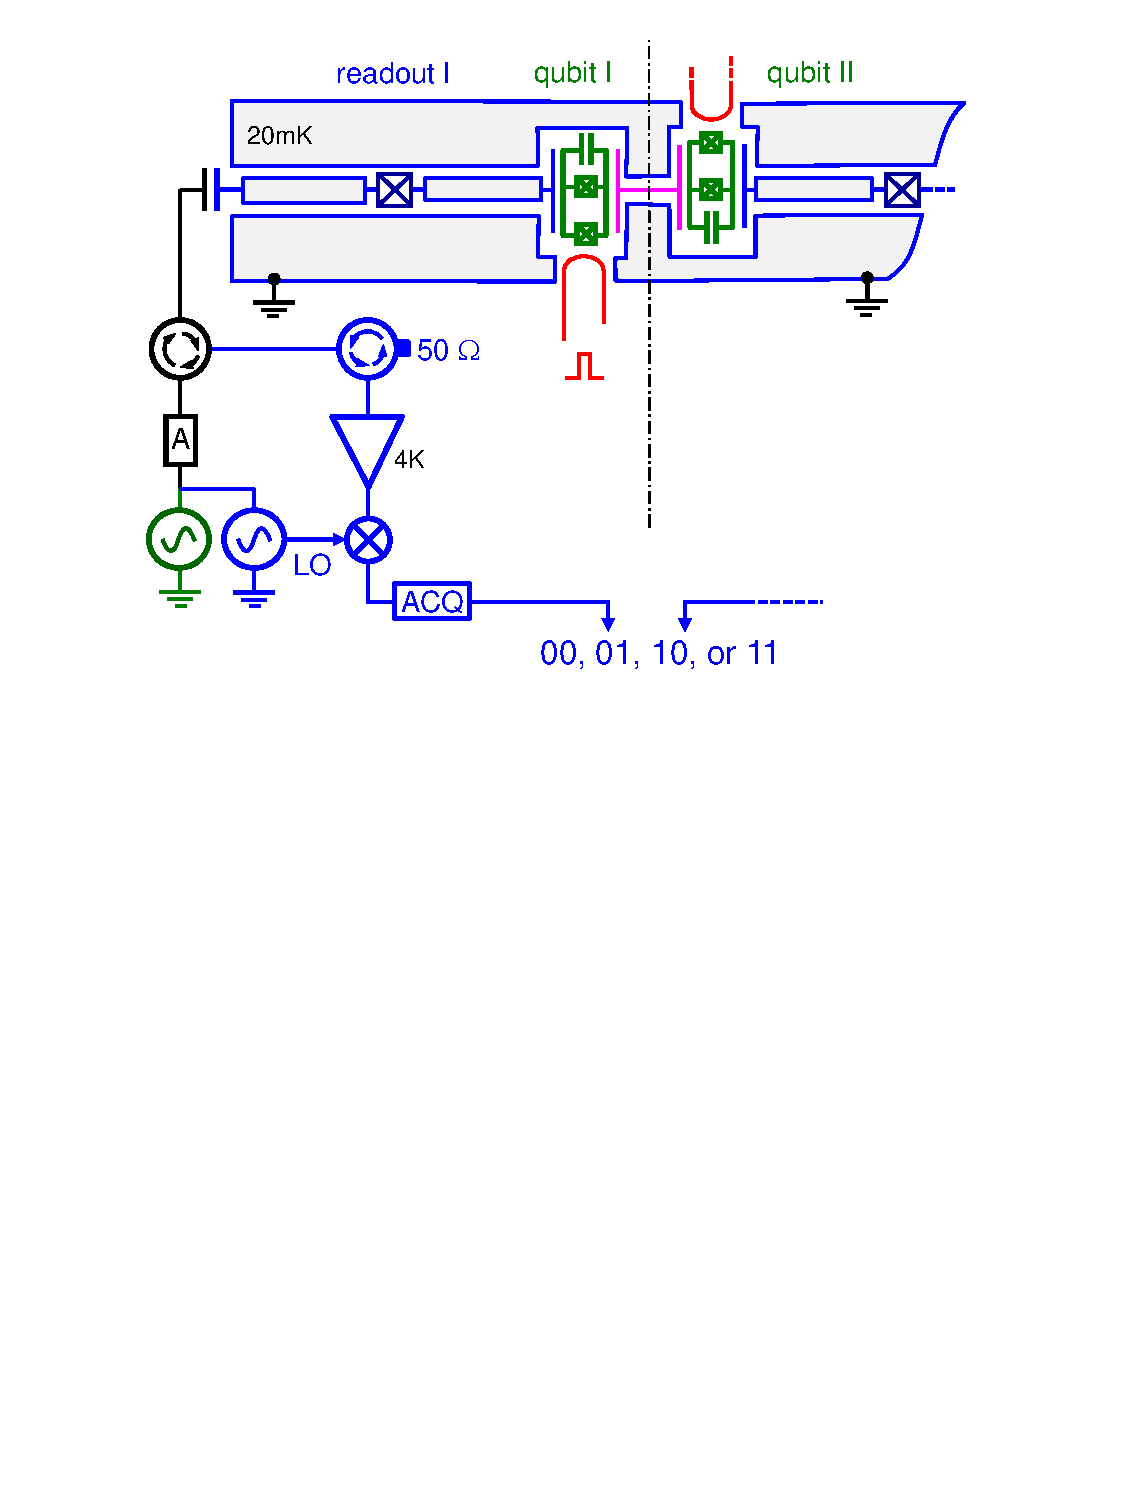
\includegraphics[width=0.75\textwidth]{./material/papers/grover/figures/2_qubit_processor_schematic}
	\caption[Circuit schematic of the realized two-qubit processor]{Circuit schematic of the two-qubit processor realized in this work, showing the two qubits in green, the qubit readouts in blue and the fast flux lines in red. Each qubit is embedded in its own nonlinear readout resonator and can be driven and read out through an individual microwave line.}
	\label{fig:two_qubit_processor_schematic}
\end{figure}

The quantum processor implemented in this work is shown in fig. \ref{fig:two_qubit_processor_schematic}. It consists of two superconducting quantum bits of the Transmon-type, each equipped with its own drive and readout circuit. The qubit readout is realized by using a nonlinear coplanar-waveguide resonator which serves as a cavity bifurcation amplifier (CBA)\citep{vijay_invited_2009} and implements a single-shot readout of the qubit state. Each qubit can be manipulated by driving it with microwave pulses through its readout resonator, allowing robust and fast single-qubit operations. The qubit frequencies can be tuned individually by fast flux lines, which allows to change the frequency each qubit over a range of several GHz. The coupling between the two qubits is realized through a fixed capacitance that connects the two top-electrodes of the qubits and implements a fixed $\sigma_{xx}$-type qubit-qubit coupling. This coupling allows us to implement a two-qubit gate and to generate entangled two-qubit states. We use this simple processor to test Bell's inequality, implement an universal two-qubit gate and perform a simple quantum algorithm that demonstrates probabilistic quantum speed-up, as will be discussed in the following sections.

\section{Demonstrating Simultaneous Single-Shot Readout}

\begin{figure}[ht!]
	\centering
		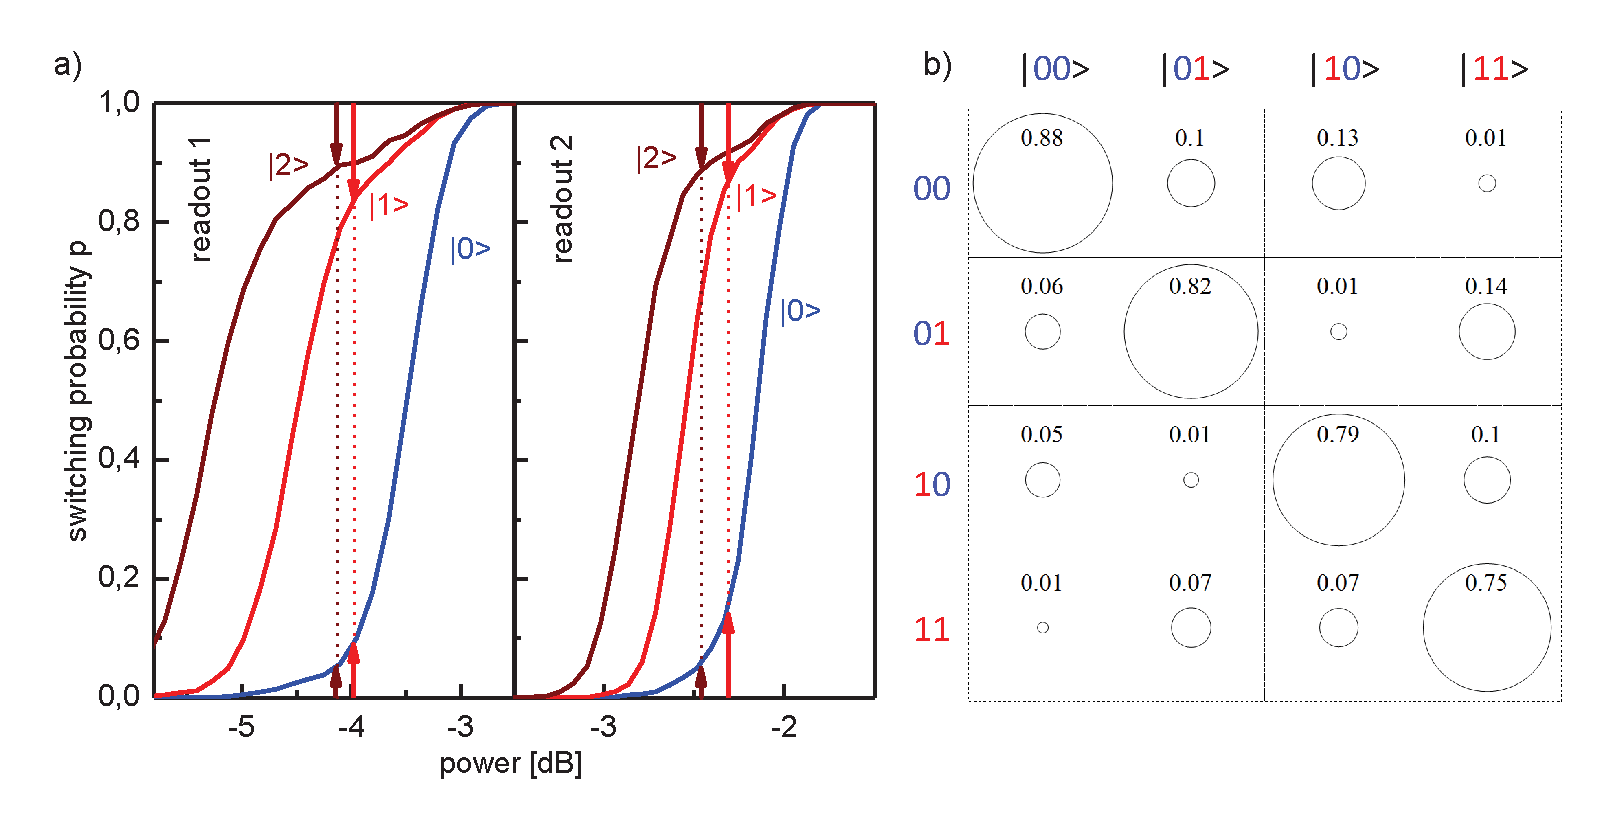
\includegraphics[width=1.\textwidth]{./material/papers/grover/figures/simultaneous_readout_characteristics}
	\caption[Switching probabilities of the two qubit readouts as a function of the readout excitation power]{a) Switching probabilities of the two qubit readouts as a function of the readout excitation power. The measurement is performed after preparing the qubits in the states $\color{blue}{\ket{0}}$, $\color{red}{\ket{1}}$ and $\color{brown}{\ket{2}}$. The readout fidelity is given as the difference in probability between the curves corresponding to the states $\color{blue}{\ket{0}}$ and $\color{red}{\ket{1}}$ or $\color{brown}{\ket{2}}$, respectively. The highest readout fidelites of 88 and 89 \% are achieved when the qubit is in state $\color{brown}{\ket{2}}$. b) Readout matrix of the two-qubit system. The matrix contains the probabilities of obtaining a given measurement result after having prepared the system in a given state. \figcomment{Replace this figure since it is not very intuitive. It would be better to show something which allows the reader to directly quantify the visibility and readout crosstalk present in the system.}}
	\label{fig:qubit_readout_characteristics}
\end{figure}

To read out the state of each qubit, a so-called cavity bifurcation amplifier \citep{siddiqi_dispersive_2006,mallet_single-shot_2009} is used. This readout technique works by capacitively coupling the qubit to a coplanar waveguide resonator which is rendered nonlinear by a Josephson junction placed in its center conductor. This nonlinear resonator can exhibit hysteretic behaviour for certain drive parameters, which can be used to map the state of the qubit to one of the bistable states of the resonator, thereby obtaining a single-shot readout. Contrary to other CQED approaches, in our setup each qubit is fitted with an individual CBA readout, allowing thus a simultaneous measurement of the full two-qubit register and therefore following closely the canonical blueprint of a quantum computer as formulated by DiVincenzo.\todo{discuss more details of the readout here...} Readout fidelitis up to 93 \% have been demonstrated using the CBA readout technique \citep{mallet_single-shot_2009} but due to design contraints only  83-85 \% fidelity have been attained in our experiments. The full characterization of the two-qubit readout is shown in fig. \ref{fig:qubit_readout_characteristics}. Fig. \ref{fig:qubit_readout_characteristics}a shows the so-called s curves of each qubit readout, which shown the working-point dependent switching probabilities of each readout with the qubits in different states. Fig. \ref{fig:qubit_readout_characteristics}b shows the full readout matrix, which connects readout switching probabilities with qubit state occupation probabilities and allows for the correction of all readout errors.

\section{Generating and Characterizing Entanglement}

\begin{figure}
	\centering
		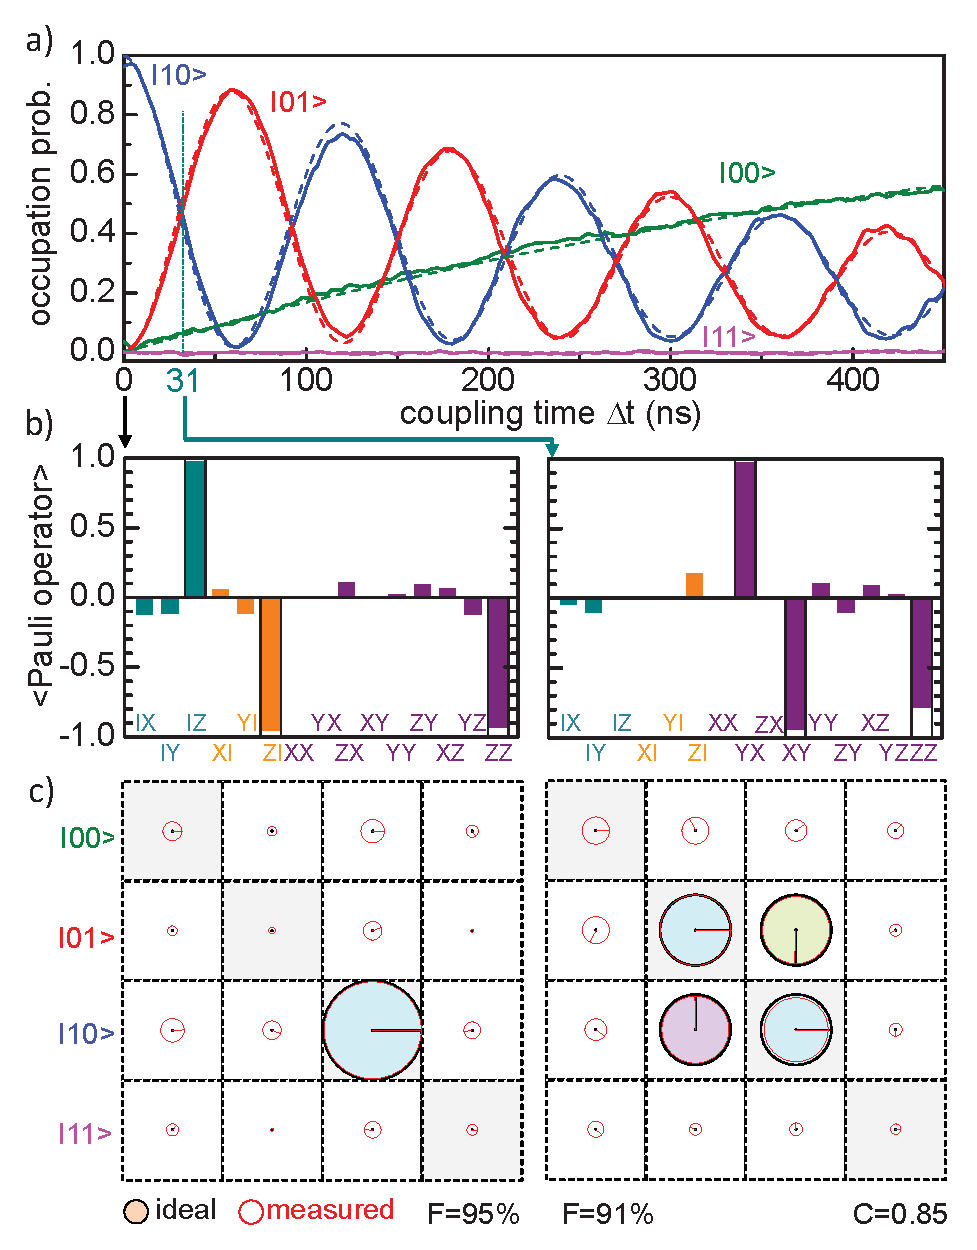
\includegraphics[width=0.7\textwidth]{./material/papers/iswap/submission1/Dewes_Figure2}
	\caption[Generating entangled two-qubit states by swapping interaction]{Energy oscillations between the two qubits induced by a resonant swapping interaction between them. a) The qubit state after switching on the swapping interaction for a given time $\Delta t$. The frequency of the oscillations corresponds to $2g = 8.7 \; \mathrm{MHz}$. b) The Pauli set of the two-qubit state measured at $0\; \mathrm{ns}$ and $31\; \mathrm{ns}$. c) The reconstructed density matrices corresponding to the two measured Pauli sets. In c), the area of each circle corresponds to the absolute value of each matrix element and the color and direction of the arrow give the phase of each element. The black circles correspond to the density matrices of the ideal states $\ket{10}$ and $1/\sqrt{2}/(\ket{10}+i\ket{01})$, respectively.\figcomment{verify sign!}}
	\label{fig:swap_interaction_state_tomography}
\end{figure}

The fixed coupling between the two qubits provides a $\sigma_{xx}$-type coupling which is only effective when the qubit frequencies are nearly resonant. Therefore, it can be switched on and off by changing the qubit frequencies, which we use to implement two-qubit gates with this system. In our processor, the effective coupling constant $g$ of the two qubits is given as $2g = 8.2 \; \mathrm{MHz}$\todo{Check if this is really $2g$!}. When using a fast fluxline pulse to abruptly tune the qubits in resonance we can switch on the qubit-qubit coupling non-adiabatically and generate an evolution operator of the form

\begin{equation}
	U(t)  =  \left( \begin{array}{cccc} 1 & 0 & 0 & 0 \\ 0 & \cos{2 \pi t g} & i\sin{2 \pi t g} & 0 \\ 0 & i\sin{2 \pi t g} & \cos{2 \pi t g} & 0 \\ 0 & 0 & 0 & 1 \end{array} \right) \label{eq:swap_evolution_operator}
\end{equation}

%explain that we stop the evolution at the right time to generate entangled states and implement a Two-qubit gate.

Switching off this interaction after a time $t_{\pi/2} = 1/8 g$ allows the creation of entangled qubit states and the implementation of a universal quantum gate, as will be explained later. Before doing this, we characterize the evoluation of the qubits during the swapping interaction by preparing them in the state $\ket{10}$, switching on the interaction for a given amount of time and measuring the qubit state directly afterwards. The resulting curve shown in fig. \ref{fig:swap_interaction_state_tomography} shows energy oscillations between the two qubits. Stopping the interaction after quarter of a period we obtain an entangled two-qubit Bell-type state that we can characterize by performing quantum state tomography. The experimental reconstruction of the density matrix of such a state corresponding approximating to the Bell-state $\ket{\psi} = 1/\sqrt{2}(\ket{01}+i\ket{10})$ is shown in fig. \ref{fig:swap_interaction_state_tomography}b. The measured fidelity of this state of 91 \% and the concurrence of 85 \% confirms that entanglement is present in the system. This entanglement can also be characterized by measuring the so-called {\it Clauser-Horne-Shimony-Holt} operator \citep{clauser_proposed_1969} on the produced state. This operator is given as

\begin{equation}
\mathrm{CHSH} = \mathrm{QS}+\mathrm{RS}+\mathrm{RT}-\mathrm{QT}
\end{equation}
with the operators $\mathrm{Q,R,S,T}$ being given as

\begin{eqnarray}
	\begin{array}{cccccccc}
		\mathrm{Q} & = & \sigma_z^1 &&& \mathrm{S} & = & \sigma_z^2\cdot \cos{\phi}+\sigma_x^2 \cdot \sin{\phi} \\
		\mathrm{R} & = & \sigma_x^1 &&& \mathrm{T} & = & -\sigma_z^2\cdot \sin{\phi}+\sigma_x^2 \cdot \cos{\phi}
	\end{array}
\end{eqnarray} 
Here, the angle $\phi$ is a parameter that should be chosen in accordance to the phase of the Bell state on which the operator is applied.

\begin{figure}[ht!]
	\centering
		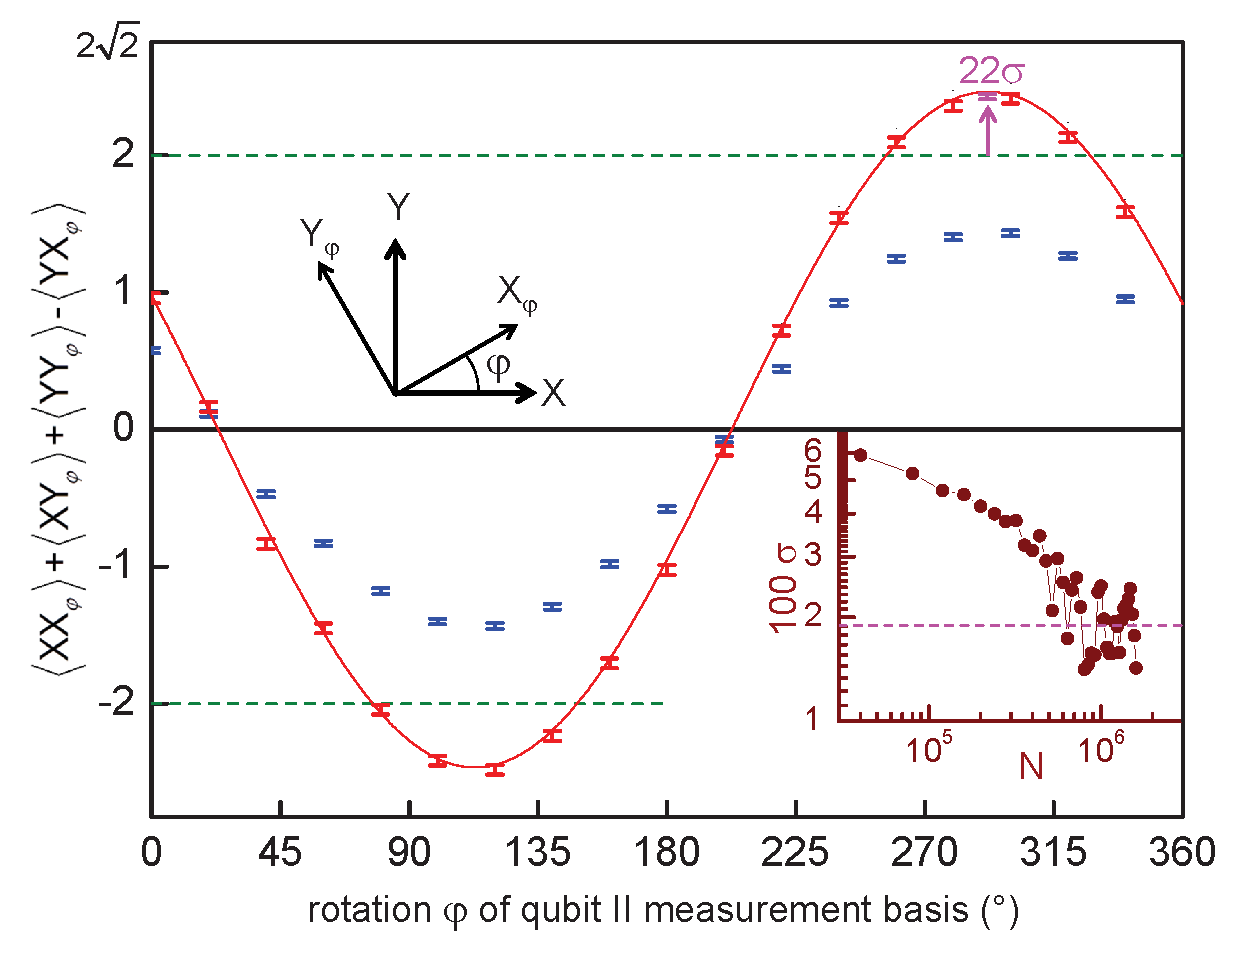
\includegraphics[width=0.7\textwidth]{./material/papers/iswap/submission1/Dewes_Figure3}
	\caption[Measurement of the CHSH operator of an entanged two-qubit state]{Measurement of the CHSH equation for an entangled two-qubit state. The renormalized CHSH expectation value (red points) exceeds the classical boundary of $2$ by a large amount. The raw measurement data (blue points) lies below this critical threshold. The inset shows the standard deviation $\sigma$ at the highest point of the curve as a function of the measurement sample size. For the highest sample count, the classical boundary is exceeded by $22$ standard deviations.\figcomment{p. 140 in cavities 6 labbook}}
	\label{fig:chsh_measurement}
\end{figure}

The expectation value $\bracket{CHSH}$ provides a test of the quantum-mechanical character of the generated state. For classical states, the maximum value is $\le 2$ but for entangled states it can reach a maximum value of $\sqrt{2}\cdot 2$. The result of a CHSH-type measurement performed on a state created by the method described above is shown in fig. \ref{fig:chsh_measurement}, showing the value of $\bracket{CHSH}$ as a function of $\phi$. We observe a violation of the classical boundary $2$ of the operator by $22$ standard deviations when correcting readout errors present in our system. However, the raw, uncorrected data fails to exceed the non-classical bound, making it impossible to close the detection loophole with our system. Nevertheless the observed violation of the equation by the renormalized state is a strong indication of entanglement in the system.

\section{Realizing a Universal Two-Qubit Quantum Gate}

\begin{SCfigure}[][ht!]
		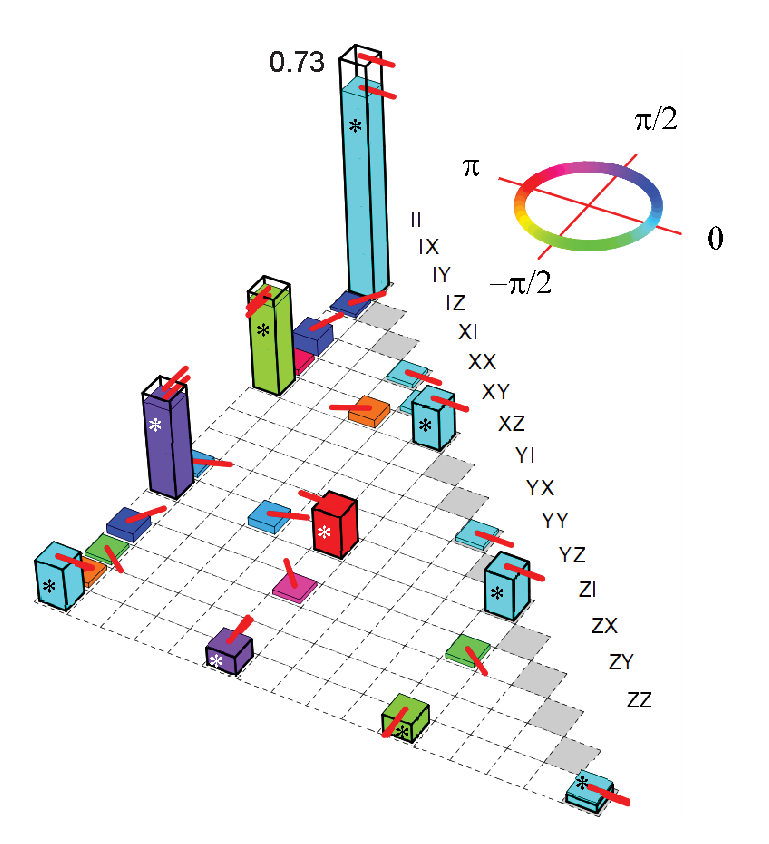
\includegraphics[width=0.65\textwidth]{./material/papers/iswap/figures/chi_matrix}
	\caption[Measured $\chi$-matrix of the $\sqrt{i\textrm{SWAP}}$ gate]{The measured $\chi$-matrix of the implemented $\sqrt{i\mathrm{SWAP}}$ gate. The row labels correspond to the indices of the $E_i$ operators, the height of each bar to the absolute value of the corresponding matrix element and the color and direction of the red arrow to the complex phase of each element. The ideal $\chi$-matrix of the $i\sqrt{\mathrm{SWAP}}$ gate is given by the outlined bars. The upper half of the positive-hermitian matrix is not shown.}
	\label{fig:gate_chi_matrix_and_errors}
\end{SCfigure}

The swapping evolution according to eq. (\ref{eq:swap_evolution_operator}) allows the implementation of a two-qubit gate. When switching on this interaction for $t_{\pi/2} = 1/8g$ we can realize the so-called $\sqrt{i\mathrm{SWAP}}$ gate, which has the representation

\begin{equation}
	\sqrt{i\mathrm{SWAP}}  =  \left( \begin{array}{cccc} 1 & 0 & 0 & 0 \\ 0 & 1/\sqrt{2} & i/\sqrt{2} & 0 \\ 0 & i/\sqrt{2} & 1/\sqrt{2} & 0 \\ 0 & 0 & 0 & 1 \end{array} \right) \label{eq:sqrt_iswap_gate}
\end{equation}
and is a universal two-qubit quantum gate. The operation and errors of our implementation of this gate can be characterized by performing quantum process tomography, yielding a gate fidelity of 90 \% . The 10 \% error in gate fidelity is caused mainly by qubit relaxation and dephasing during the gate operation and only marginally by deterministic preparation errors, as will be discussed in the main text of the thesis. Fig. \ref{fig:gate_chi_matrix_and_errors} show the measured $\chi$ matrix of the implemented gate. The achieved fidelity of the gate operation is sufficient to allow the implementation of a simple quantum algorithm with our processor, as will be discussed in the following section.
 
\section{Running a Quantum-Search Algorithm}

\begin{figure}[ht!]
	\centering
		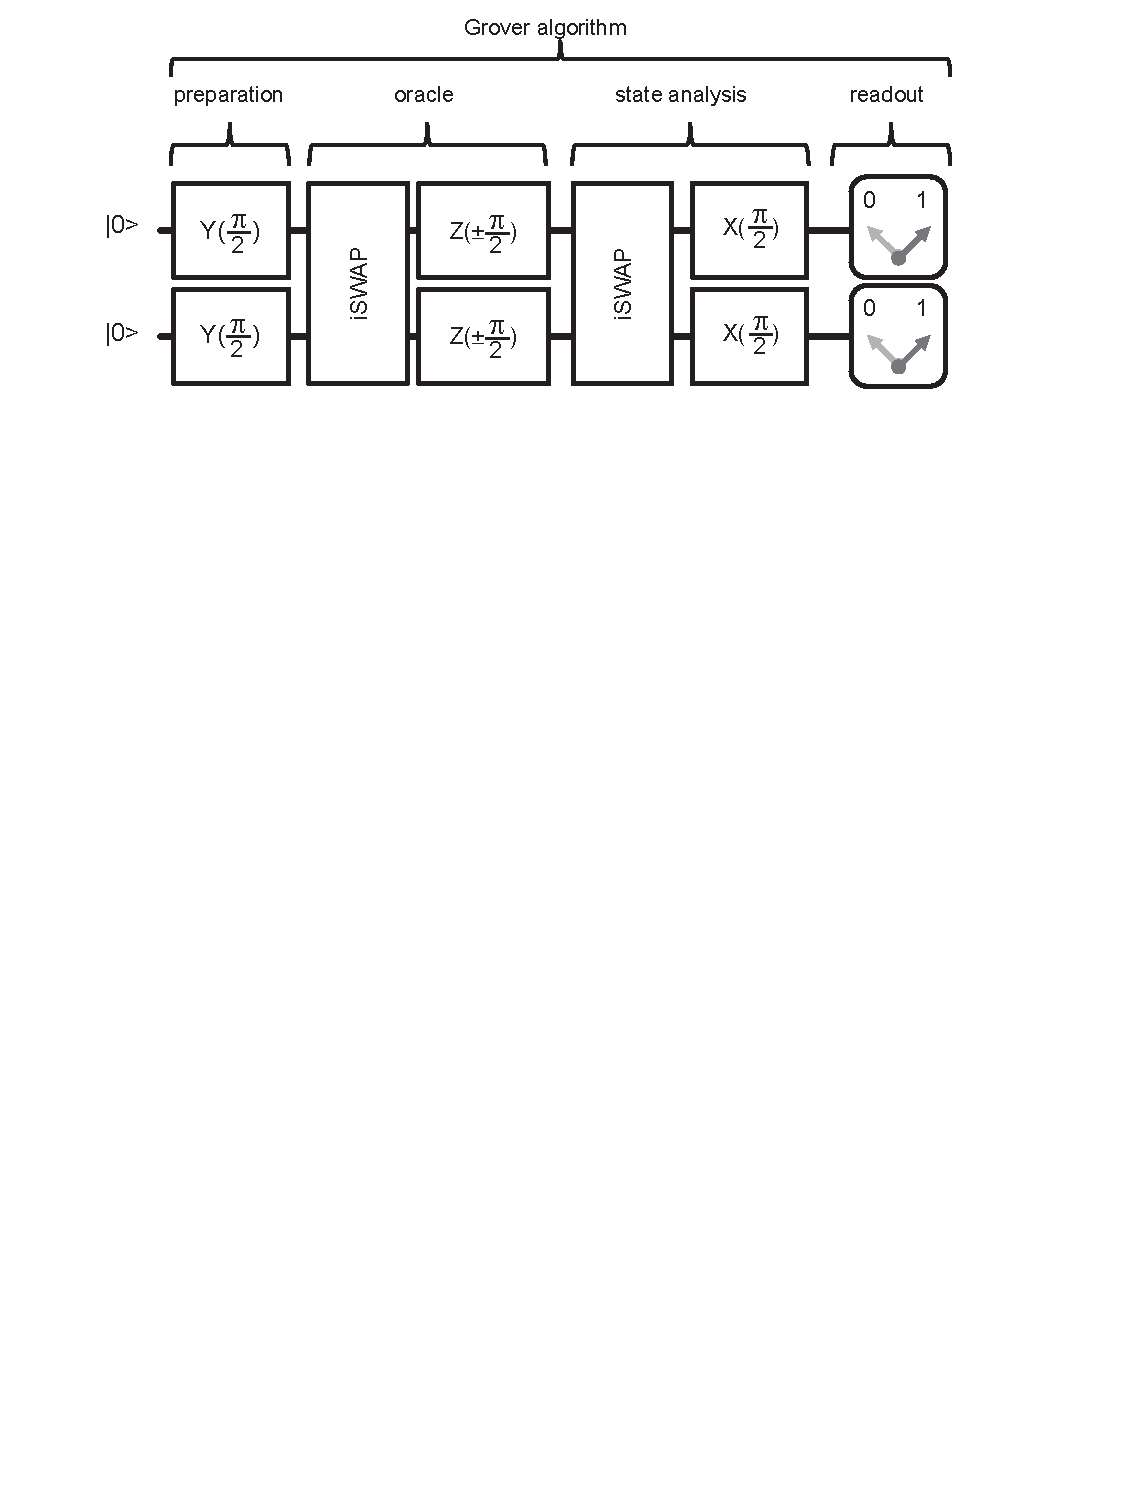
\includegraphics[width=0.8\textwidth]{./material/papers/grover/figures/grover_algorithm_schematic}
	\caption[Schematic of the implementation of Grovers search algorithm]{Schematic of the implementation of Grovers search algorithm on a two-qubit quantum processor. The algorithm consists in preparing a probe state, applying the quantum oracle to this state and analyzing the resulting output state to extract the information on the oracle operator.} 
	\label{fig:grover_algorithm_schematic}
\end{figure}

In this work we use the quantum gate implemented above to run a compiled version of Grover's search algorithm \citep{Grover_Quantum_1997}. The implemented version of the algorithm works in the basis of two qubits $x_i \in \{\ket{00},\ket{01},\ket{10},\ket{11}\}$ and  can distinguish between four different {\it oracle functions} $f(x)$ that each tag on one of the basis states $x_j$. Since the Grover algorithm for 2 qubits requires only one evaluation of the function $f(x)$ to determine which state has been marked it is faster than any conceivable classical algorithm, thus demonstrating the concept of quantum speed-up. The schematic of our version of Grover's algorithm is shown in fig. \ref{fig:grover_algorithm_schematic} and involves two $i\mathrm{SWAP}$ gates and three single-qubit operations along with a single-shot qubit readout at the end of the algorithm. We implemented all steps of this algorithm with our two-qubit processor and performed quantum state tomography after each step to reconstruct the quantum state at different points in the algorithm. Fig. \ref{fig:grover_density_matrices_state_1} shows the experimentially measured density matrices when running the algorithm with an oracle that marks the state $\ket{00}$. State tomographies are shown after applying the generalized Hadamard transform, after applying the quantum oracle and after the final step of the algorithm. This reconstruction of the quantum state using quantum state tomography does not however allow to demonstrate quantum speed-up, which requires individual single-shot readout of the qubit register, which will be discussed in the following section.

\begin{figure}[ht!]
	\centering
		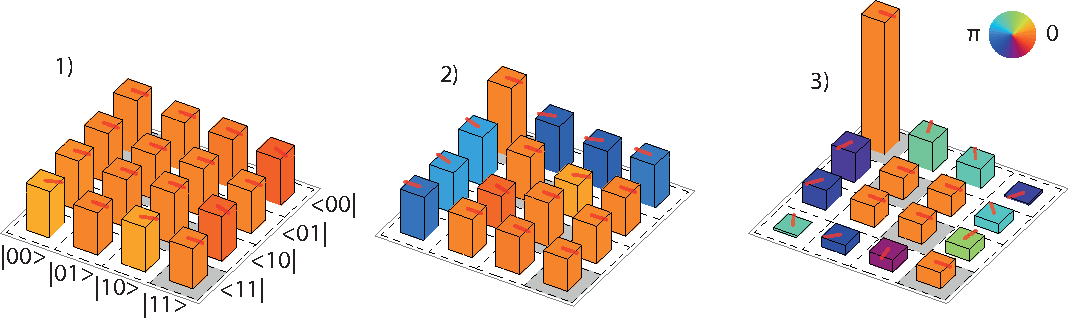
\includegraphics[width=1.\textwidth]{./material/figures/2-qubit-processor/grover/grover-density-matrices-state-1}
	\caption[Measured density matrices when running Grover's algorithm]{Measured density matrices when running Grover's search algorithm with a search oracle marking the state $\ket{00}$. 1) shows the state after the generalized Hadamard transform, 2) after applying the quantum oracle and 3) after the final step of Grover's algorithm.} 
	\label{fig:grover_density_matrices_state_1}
\end{figure}


\section{Demonstrating Quantum Speed-Up}

The main interest of running a quantum algorithm is to obtain an advantage in the run-time in comparision with a classical algorithm, the so-called {\it quantum speed-up}. To characterize this quantum speed-up as obtained with our processor, we run Grovers algorithm for all four possible oracle functions and directly readout out the qubit state after the last step of the algorithm, without correcting any readout errors. When averaging the results of such individual runs of the algorithm we can then obtain its single-run fidelity, which --for our processor-- ranges between 52 and 67 \%, depending on the state which is  marked by the quantum oracle, as shown in fig. \ref{fig:grover_single_shot_probabilities}. These results clearly demonstrate quantum speed-up in this system, although the achieved success probability is considerably lower than the theoretically possible value of 100 \% . The reduced fidelity is mainly due to relaxation and decoherence of the qubit state during the running of the algorithm and to a very small degree due to errors in the pulse sequence and drifts in the measurement equipment.

\begin{figure}[ht!]
		\centering
		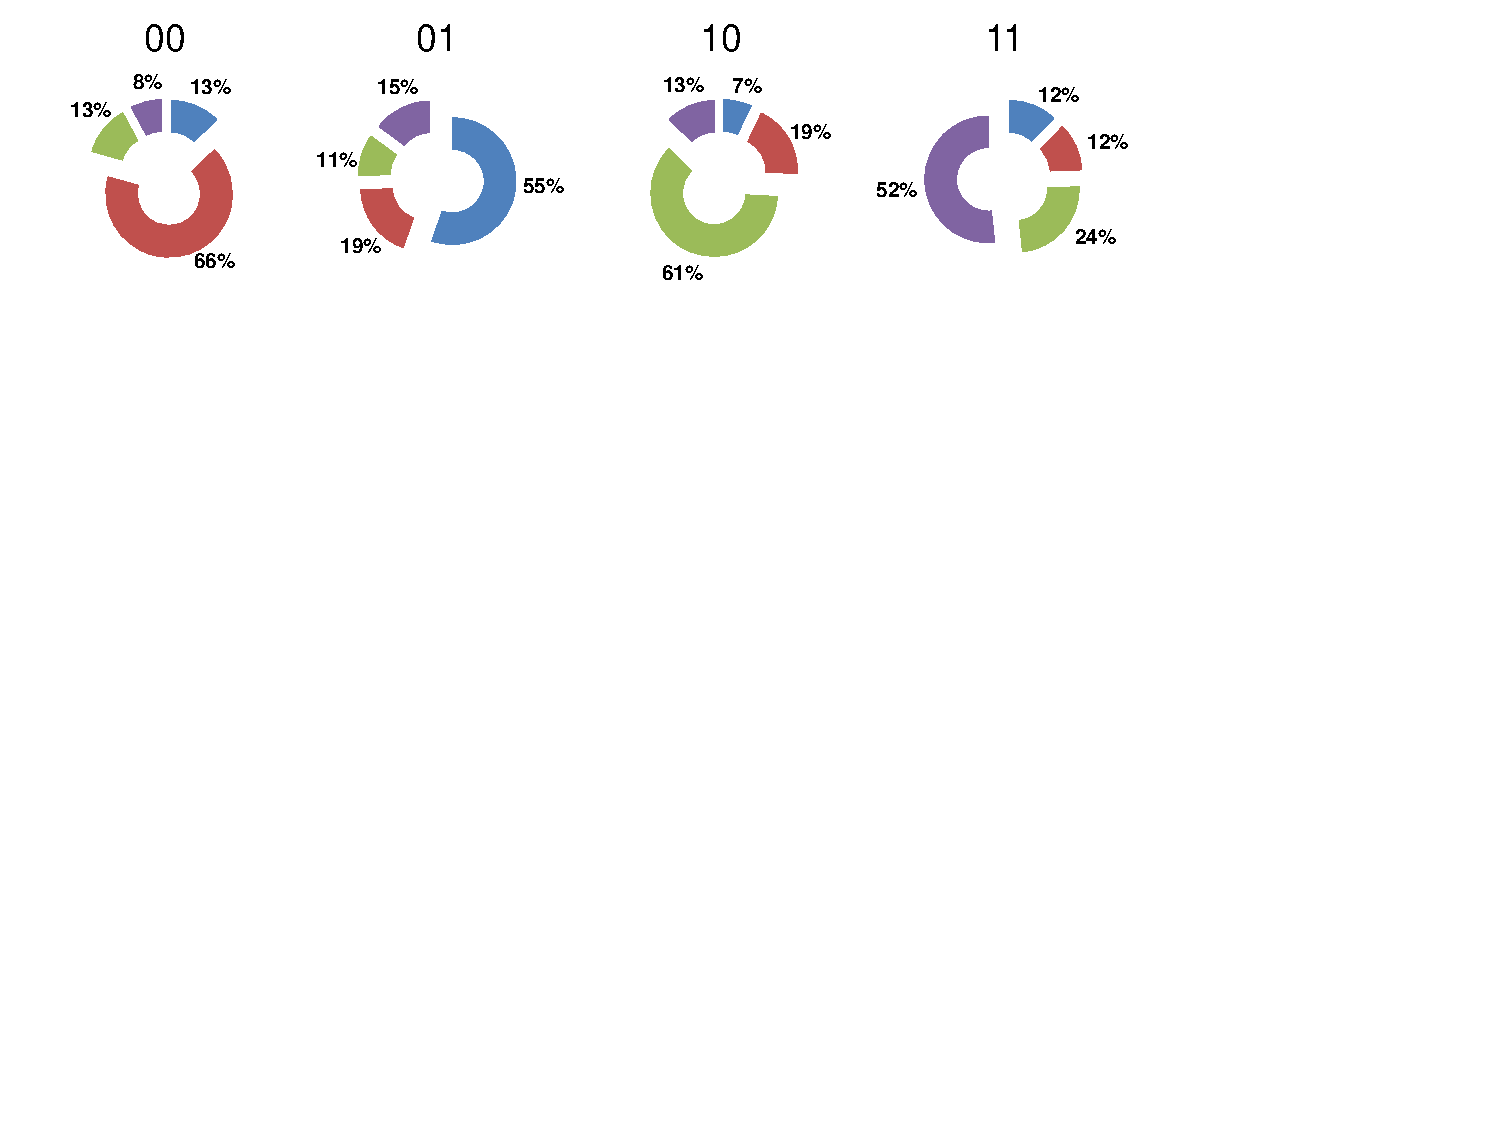
\includegraphics[width=1.0\textwidth]{./material/papers/grover/figures/grover_algorithm_single_shot_probabilities}
	\caption[Single-run results of the Grover search algorithm]{Single-run results when running the Grover search algorithm on our two-qubit quantum processor. Shown are the probabilities of obtaining the results $00,01,10,11$ as a function of the oracle function provided to the algorithm, indicated by the number on top of each graph. In all four cases, the success probability of the algorithm is $> 50 \%$, thus outperforming any classical algorithm in the number of calls to the oracle function.}
	\label{fig:grover_single_shot_probabilities}
\end{figure}

\section{Designing a Scalable Quantum Computing Architecture}

After having demonstrated the different building blocks of a superconducting, Transmon-based quantum processor it remains to be shown that larger-scale quantum-computing beyond two qubits is possible with this system. This work therefore pursued the realization of a more scalable qubit architecture using systems of up to six qubits coupled through a so-called ``quantum bus'' \citep{majer_coupling_2007}. The details of this novel architecture are discussed in the following sections.

The approach for scalable quantum computing with superconducting qubits pursued in this work consists of a system of many individual Transmon qubits equipped with individual JBA-based readouts, a multiplexed drive and readout circuit and a fixed qubit-qubit coupling mediated through a high-Q CPW resonator. As before, each qubit possesses a fluxline for fast frequency control. The readout and drive signals are send to all the qubits in parallel through a multiplexed transmission line. In this approach, the qubit and readout parameters, couplings and frequencies have to be carefully to avoid unwanted coupling between individual qubits and readouts and to allow the implementation of robust quantum gates between individual qubits. In this work we realized a 4-qubit chip and characterized it experimentally. The results of these experiments will be discussed in the main text of this thesis.

\begin{figure}[ht!]
  \centering
	\includegraphics[width=1.\textwidth]{"./material/figures/scalable-architecture/scalable architecture - schematic"}
	\caption[...]{...}
\end{figure}


\chapter{Theoretical Foundations} \label{chapter:theory}

In this chapter we provide the reader with the minimum conceptual background and theoretical building blocks necessary  to understand this thesis work. We begin our discussion with a general overview of classical and quantum information processing with a Turing machine, followed by an introduction to superconducting quantum circuits. We summarize the method to quantize electrical circuits and apply it to Cooper pair box devices, and in particular to the Transmon that will be used to implement the qubit register of our quantum processor. We then present coplanar waveguide resonators, and introduce circuit quantum electrodynamics on the example of a transmon coupled to a such a resonator. Finally, we consider the case of a nonlinear resonator used as a Josephson bifurcation amplifier since we use such a readout device in our processor architecture.

\section{Classical \& Quantum Information Processing}

\begin{SCfigure}
	\includegraphics[width=8cm]{"./material/figures/introduction/bloch_sphere"}
	\caption{The Bloch sphere representation of a qubit state $\ket{\psi} = \cos{\frac{\theta}{2}}\ket{0}+e^{i\phi}\sin{\frac{\theta}{2}}\ket{1}$. The state $\ket{\psi}$ is fully characterized by specifying its ``latitude'' and ``azimuth'' angles $\theta$ and $\phi$. Pure quantum states will always lie on the surface of the Bloch sphere, whereas mixed quantum states can also lie anywhere inside the sphere.}
	\label{fig:BlochSphere}
\end{SCfigure}

By definition, computing designates the activity of using computer hardware and software to process information, or {\it data}. Classical information processing can be divided in so-called {\it analog and digital information processing}, the former being based on continuously changeable physical quantities whereas the latter is based on incrementally changeable quantities. The fundamental unit of digital information processing is the so-called {\it bit}, which represents a Boolean (true/false) information. The discipline of theoretical computer science has been created to investigate the fundamental limits and properties of classical information processing. One of the main foundational theorems of theoretical computer science is the so-called {\it Church-Turing thesis} which provides a universal computing model by saying (basically) that everything which is computable can be efficiently computed using a {\it Turing machine}. Such a Turing machine, in turn, is a simple theoretical device which is able to run programs that operate on a discrete set of data using a well-specified set of operations. The Turing machine is universal in the sense that any other classical computing device can be efficiently emulated using a Turing machine with the appropriate program and data.

\smallskip

In the early 1980, Richard Feynman discovered that a classical Turing machine as described above would be unable to efficiently simulate a quantum-mechanical system \citep{feynman_simulating_1982}. He introduced the concept of a {\it quantum Turing machine} that would be able to simulate quantum-mechanical systems in an efficient manner. A few years later, David Deutsch took up Feynman's idea and developed an information processing framework based on quantum mechanics \citep{deutsch_quantum_1985}, coining the terms {\it quantum computing} and {\it quantum information processing}. He showed that by making use of different properties of quantum mechanics, namely, the superposition principle and entanglement, one could solve certain mathematical problems faster than possible with any classical computer \citep{deutsch_quantum_1985}. The work by Deutsch created a large interest in the physics community and led to a huge theoretical and experimental effort aimed at realizing an operational quantum computer and developing quantum algorithms for relevant real-world problems.

\section{Principles of "Conventional" Quantum Computing}

The first scheme imagined for quantum information processing is directly inspired from the classical digital Turing machine: information is stored in a set of quantum two level systems, the {\it quantum bits} or {\it qubits}, forming a quantum register, which is manipulated by sequentially applying unitary (and possibly non-unitary) operators to subsets of qubits in the register, typically one or two. As for a classical Turing machine, any arbitrary operation of this quantum processor can be decomposed as a sequence of gate operations chosen from a surprisingly small set of gates, said universal. The power of such a machine comes from the gates operating on superposed states, which provides an intrinsic parallelism in the processing.
\smallskip
This {\it quantum gate} approach is the method relevant to the present thesis work, and we ignore other approaches introduced more recently such as {\it one-way quantum computing} \citep{raussendorf_one-way_2001}, {\it adiabatic quantum computing} \citep{farhi_quantum_2000} or {\it topological quantum computing} \citep{kitaev_fault-tolerant_2003}. In this section we introduce very briefly quantum bits and quantum gates, as well as some examples of quantum algorithms that are relevant to this work.


\subsection{Quantum Bits and registers}

As in classical computing, one can define in quantum computing a fundamental unit of information: the qubit. Such a qubit is a quantum-mechanical two-level system that can be put in any superposition
%
\begin{equation}
\ket{\psi} = \cos{\frac{\theta}{2}}\ket{0}+e^{i\phi}\sin{\frac{\theta}{2}}\ket{1}
\end{equation}
%
of its two states $\ket{0}$ and $\ket{1}$.
As can be seen, any state can be described by a pair of real numbers $\theta$ and $\phi$ that characterize the amplitude of each of the two basis states and the phase between them. A useful and intuitive representation of such a single-qubit state is the so-called {\it Bloch sphere representation}, shown in fig. \ref{fig:BlochSphere}. The north and south poles of this sphere correspond by convention to the qubit states $\ket{0}$ and $\ket{1}$ (or vice versa). In this representation, any pure state $\ket{\psi}$ is located on a unit sphere. All states lying on the sphere between those two correspond to superposition states, which are characterized by their ``latitude'' and ``azimuth'' angles $\theta$ and $\phi$. 

\smallskip

\smallskip
If the qubit state is not pure but is a mixed state given by the complete set of probabilities ${p_{i}}$ to find it in one of the pure states  ${\ket{\psi_{i}}}$, it is characterized by the density matrix $\rho_{mixed} = \sum\limits_i p_i \rho_i$ with $\rho_i=\ket{\psi_{i}}\bra{\psi_{i}}$ the density matrix of the pure state $\ket{\psi_i}$. These $\rho$'s are Hermitian $2\times 2$ matrices with non-negative eigenvalues and can be written as
%
\begin{equation}
\rho = \left( \begin{array}{cc} \rho_{00} & \rho_{01} \\ \rho_{01}^* & \rho_{11} \end{array} \right),
\end{equation}
%
in the ${\ket{0},\ket{1}}$ basis, with $\rho_{00}$ and $\rho_{11}$ being real numbers and $\rho_{01}$ a complex number. For any state, the matrix has a unity trace $\mathrm{Tr}(\rho)=1$, for pure states we have $\rho=\rho^2$ in addition. The expectation values $\langle A \rangle$ of any operator $A$ acting on the density matrix $\rho$ is given as $\mathrm{Tr}(\rho A)$.

\smallskip

A mixed single-qubit state $\rho$ can also be represented on the Bloch sphere. For this, we decompose $\rho = c_i\sigma_I+c_x\sigma_x+c_y\sigma_y+c_z\sigma_z$, where $c_{i,x,y,z}$ are complex coefficients and the Pauli matrices $\sigma_I,\sigma_x,\sigma_y,\sigma_z$ are
%
\begin{align}
  \sigma_I  =  \left( \begin{array}{cc} 1 & 0 \\ 0 & 1 \end{array} \right)
 & &  \sigma_x  =  \left( \begin{array}{cc} 0 & 1 \\ 1 & 0 \end{array} \right)
  & & \sigma_y  =  \left( \begin{array}{cc} 0 & -i \\ i  &  0\end{array} \right)
  & & \sigma_z  =  \left( \begin{array}{cc} 1 & 0 \\ 0 & -1 \end{array} \right).
\label{eq:pauli_operators}
\end{align}
% 
We can then plot the vector $(c_x,c_y,c_z)$ in the Bloch sphere. The length of this vector decreases from 1 for a pure state down to 0 for a completely mixed state.

\smallskip

Quantum states with more than one qubit cannot be described anymore using Bloch spheres but are easily described with density matrices of dimension $2^n\otimes 2^n$ in the computational basis $\ket{q_1\hdots q_n}=\ket{q_1}\otimes\ket{q_{2}}\hdots\otimes\ket{q_n}$.For example, a two-qubit Bell state of the form $\ket{\psi_+}=(\ket{01}+\ket{10})/\sqrt{2}$ can be written as
%
\begin{equation}
\rho_{\psi_+} = \frac{1}{2}\left( \begin{array}{cccc} 0 & 0 & 0 & 0 \\ 0 & 1 & 1 & 0 \\ 0 & 1 & 1 & 0 \\ 0 & 0 & 0 & 0 \end{array} \right)_{(\ket{00},\ket{01},\ket{10},\ket{11})}
\end{equation}
%
whereas a completely mixed state of 50 \% $\ket{01}$ and 50 \% $\ket{10}$ is represented by the matrix
%
\begin{equation}
\rho_{\psi_+} = \frac{1}{2}\left( \begin{array}{cccc} 0 & 0 & 0 & 0 \\ 0 & 1 & 0 & 0 \\ 0 & 0 & 1 & 0 \\ 0 & 0 & 0 & 0 \end{array} \right)_{(\ket{00},\ket{01},\ket{10},\ket{11})}
\end{equation}
%

\subsection{Quantum Gates}

Analogously to classical information processing one defines {\it quantum gates} that act on individual or multiple qubits and allow us to process information. Such a quantum gate can be described as a unitary operator acting on a part of the Hilbert space representing the qubit register. Theoretically there is an infinite number of possible quantum gates, however in order to describe all possible quantum operations that can be performed on a qubit register of arbitrary length it is sufficient to defined a so-called {\it universal set of quantum gates}. Such a set contains a small number of quantum gates that can, by concatenation, produce any arbitrary unitary quantum operator, as shown by the so-called {\it Solovay-Kitaev theorem} \citep{nielsen_quantum_2000,dawson_solovay-kitaev_2005}. Such a universal gate set that will be especially relevant to this work consists of the three single-qubit rotation matrices
%
\begin{eqnarray}
   R_x(\theta)  & = & e^{-i\sigma_x\frac{\theta}{2}} \\ 
   R_y(\theta)  & = & e^{-i\sigma_y\frac{\theta}{2}} \\ 
   R_z(\theta)  & = & e^{-i\sigma_z\frac{\theta}{2}} 
\label{eq:universal_single_qubit_gates}
\end{eqnarray}
%
together with the so-called $\sqrt{i\mathrm{SWAP}}$
%
\begin{equation}
\sqrt{i\mathrm{SWAP}} = \left( \begin{array}{cccc} 1 & 0 & 0 & 0 \\ 0 & 1/\sqrt{2} & i/\sqrt{2} & 0 \\ 0 & i/\sqrt{2} & 1/\sqrt{2} & 0 \\ 0 & 0 & 0 & 1  \end{array}  \right)_{(\ket{00},\ket{01},\ket{10},\ket{11})}
\end{equation}
%
By applying the $\sqrt{i\mathrm{SWAP}}$ operation twice we obtain the $i\mathrm{SWAP}$ quantum gate, which is, by itself, \textbf{not} a universal quantum gate but which is nevertheless used in some practical quantum algorithms:
%
\begin{equation}
i\mathrm{SWAP} = \left( \begin{array}{cccc} 1 & 0 & 0 & 0 \\ 0 & 0 & i & 0 \\ 0 & i & 0 & 0 \\ 0 & 0 & 0 & 1  \end{array}  \right)_{(\ket{00},\ket{01},\ket{10},\ket{11})}
\end{equation}
%

This universal set it not minimal, since in principle two single-qubit gates with a fixed rotation angle (e.g. $R_x(\pi/4)$ and $R_y(\pi/4)$) together with a universal two-qubit gate would be sufficient to form a universal set of gates \citep{dawson_solovay-kitaev_2005}. However, it is often advantageous if one can use single-qubit rotations with arbitrary rotation angles around all three axes of the Bloch sphere since it can significantly reduce the number of gates required to implement a given unitary operation.

\subsection{Quantum Algorithms}

The interest in quantum computing is mainly due to the fact that certain problems can be solved faster on a quantum computer than on a classical computer. By faster we mean here that the order $\cal{O}$ of the run time of the algorithm increases faster on a classical computer than on a quantum computer as a function of the problem size, i.e. the number of bits needed to encode the problem. Up to this day it has not been demonstrated that a quantum computer can perform all tasks faster than a classical computer. However, a small number of real-world problems have been found that can be solved exponentially to polynomially faster on a quantum computer. Here we cite only the two most ``famous'' ones:

\begin{enumerate}
\item \textbf{The Shor Factorization Algorithm} Developed by Peter Shor in 1994 \citep{shor_algorithms_1994,shor_polynomial-time_1995}. This algorithm can factorize a binary number of length $N$ into its prime factors in $\begin{mathcal}O\end{mathcal}(\log^3{N})$ steps, therefore exponentially outperforming any known classical factorization algorithm. There is large interest in this algorithm since products of large prime numbers are routinely used in asymmetric cryptography.
\item \textbf{The Grover Search Algorithm}: Discovered by Lov Grover in 1996 \citep{grover_fast_1996}, this search algorithm can find a single well-defined state in an unsorted database of size $N$ in $\begin{mathcal}O\end{mathcal}(\sqrt{N})$ steps, being hence quadratically faster than a classical search algorithm (http://en.wikipedia.org/wiki/Quantum\_algorithm).
\end{enumerate}

\subsection{Quantum Simulation}

Another domain of interest for quantum computers is the so called {\it quantum simulation} \citep{lloyd_universal_1996}. Here the goal is to simulate the behavior of an arbitrary quantum system using a quantum computer by either engineering the quantum computer in direct analogy with the system being modeled (so called {\it analog quantum simulation}) or by numerically simulating the Hamiltonian of the quantum system on a general-purpose quantum computer (so-called {\it digital quantum simulation}). Since no classical computer can simulate a quantum system efficiently, there is a large interest in quantum simulation, especially in the fields of biology \& chemistry \citep{barreiro_open-system_2011}, quantum field theory \citep{gerritsma_quantum_2010,freedman_simulation_2002} and many-body physics \citep{simon_quantum_2011}.

\subsection{Realization of a Quantum Computer}

To realize a working quantum computer, it is necessary to implement highly coherent qubits that can be manipulated, read out and coupled with high fidelity. So far, no fully working quantum computer has been experimentally demonstrated. However, larger progress towards its realization has been achieved in the last decade. Promising approaches for its realization include, among others, ions trapped in magnetic and electric fields \citep{monroe_demonstration_1995,cirac_quantum_1995}, nuclear magnetic resonance of organic molecules \citep{jones_nmr_2001,vandersypen_experimental_2001}, cold atomic gases \citep{briegel_quantum_2000}, photonic circuits \citep{knill_scheme_2001}, semiconductor circuits \citep{loss_quantum_1998} and, last but not least, superconducting circuits. Since this work treats only superconducting qubits, we focus our attention on them. We explain how we can realize a reliable qubit using superconducting structures and how we can implement circuits to manipulate, couple and read out the qubit state.

\section{Superconducting Quantum Circuits}

In this section we discuss several types of superconducting circuit elements that are most relevant to this work. First, we introduce the reader to the Josephson junction, which is the device we use to realize superconducting qubits and amplifiers. Then, we present a general method for the quantization of arbitrary electrical circuits that we use afterwards to perform canonical quantization of our circuits. We use this method to derive the Hamiltonian of the Cooper pair box and treat the Transmon qubit as a special case. Afterwards, we discuss the properties of transmission lines and transmission line resonators that we use extensively for implementing readout and coupling elements in our qubit design. Then we give a short overview of the field of circuit quantum electrodynamics and finally introduce the reader to the Josephson and cavity bifurcation amplifiers that we use for our qubit readout.

\subsection{The Josephson junction}

The core element used to construct quantum circuits is the so-called {\it Josephson junction}, being equivalent in significance to the transistor in classical circuits. A Josephson junction is based on the so-called Josephson effect \citep{josephson_possible_1962}, which states that between two superconductors connected through an insulating barrier, a supercurrent
%
\begin{equation}
I = I_c\sin{\varphi}
\end{equation}
%
will flow, depending on the difference $\varphi = \varphi_2-\varphi_1$ between the gauge-invariant superconducting phases $\varphi_1$ and $\varphi_2$ at each side of the link. $I_c$ is the so-called {\it critical current} of the Josephson junction, which is the maximum current that it can support without transitioning to a resistive state. $\varphi$ is related to the instantaneous voltage between the electrodes of the junction as
%
\begin{equation}
V = \varphi_0\frac{\partial \varphi}{\partial t},
\end{equation}
%
where $\varphi_0 =\hbar/2e \approx 3.26\times 10^{-16}\;\mathrm{Wb}$. These two simple equations yield a system exhibiting a  wealth of interesting physical phenomena which are used today in various applications such as quantum limited amplifiers \citep{vijay_invited_2009}, generation of Terahertz radiation \citep{ozyuzer_emission_2007} and voltage standards \citep{levinsen_inverse_1977}. The energy associated with the phase difference across the Josephson junction is
%
\begin{equation}
E = E_J\cdot(1-\cos{\varphi})
\end{equation}
%
where $E_J = I_c\varphi_0$ is the so-called {\it Josephson energy}. In addition to this Josephson energy, the junction usually has an electrostatic energy associated to its capacitance (formed by its two electrodes) given as $E_C = Q^2/2C$, with $\pm|Q|$ being the charge accumulated on each of the electrodes of the junction.

\smallskip

For currents $I\ll I_c$, the Josephson junction behaves approximately like a nonlinear inductance
%
\begin{equation}
L_J(\varphi) = \frac{\varphi_0}{I_c \cos{\varphi}} \approx L_{J0}\left[1+\frac{\varphi^2}{2}+\begin{mathcal}O\end{mathcal}(\varphi^4)\right],\label{eq:josephson_inductance}
\end{equation}
%
where $L_{J0}=\varphi_0/ I_c$ is the so-called {\it Josephson inductance}. 

\smallskip

Using the potential and capacitive energies of the Josephson junction, we can formulate the quantum Hamiltonian of the junction, which is
%
\begin{equation}
\hat{H} = \frac{1}{2C}\hat{Q}^2+E_J(1-\cos{\hat{\varphi}}),
\end{equation}
%
where $\hat{\varphi}$ and $\hat{Q}$ are now conjugate quantum operators that, in analogy to a classical pendulum, play the role of position and momentum for the Josephson junction. In the limit of small angles $\varphi$, the Hamiltonian becomes that of a quantum harmonic LC oscillator. The nonlinearity present in the system is a key ingredient for realizing a Josephson junction qubit since it makes it possible to drive transitions between the first two quantum states of the device without also exciting higher quantum states, as would be the case for a quantum harmonic oscillator.

\subsection{Quantization of Electrical Circuits}

In this section we outline a general method to treat arbitrary electrical circuits as the ones discussed before within the framework of quantum-mechanics, hence {\it quantizing} them. This introduction on circuit quantization presented in this chapter is based on an article by B. Yurke \citep{yurke_quantum_1984} and an article by M. Devoret \cite{devoret_quantum_1995}. A more specific example of circuit quantization can be found in \citep{burkard_multilevel_2004}.

\smallskip

An electrical circuit is fully characterized by the parameters of its elements and its topology. The latter can be described as a set of nodes $j$ connected by a number of branches $i$ formed by the circuit elements . In classical circuit theory, each branch is described by a voltage $V_i$ between its ends and a current $I_{i}$ flowing through it. The Kirchhoff laws demand that the sum of the branch voltages $V_i$ along any closed path in the circuit must be zero and that the sum of currents flowing in and out of each node must be zero. For quantization it is usually more convenient to replace voltages and currents with branch charges and fluxes that are defined as
%
\begin{eqnarray}
\Phi_i(t) & = & \int\limits_{-\infty}^t V_i(t') dt' ;\\
Q_i(t) & = & \int\limits_{-\infty}^t I_i(t') dt'.
\end{eqnarray}
%
The Kirchhoff laws now write
%
\begin{align}
\sum\limits_{i} Q_i  =  Q_c & & , & & \sum\limits_{i}\Phi_i = \Phi_c \label{eq:kirchhoff_charge}
\end{align}
%
where $Q_c$ and $\Phi_c$ are constants and where the first sum is over charges $Q_i$ of all elements connected to a certain node and the second one is over all branches forming a closed loop in the circuit. We can obtain a complete set of node and branch equations for any given circuit by constructing the so-called {\it spanning tree} of the circuit, which is a tree in which all nodes are connected to an arbitrarily chosen {\it ground node} by one unique path \citep{devoret_quantum_1995}. From the spanning tree we can obtain a complete set of branches and the corresponding Kirchoff equations for the fluxes $\Phi_i$ around them. Together with the set of Kirchhoff equations for the charges at each node, we can use this system of equations to eliminate unnecessary circuit variables and obtain a description of the circuit using a minimal set of degrees of freedom. Now, to quantize a circuit made up of non-dissipative elements we can follow the method given in \cite{yurke_quantum_1984}, writing the Lagrangian (using the reduced set of variables) as 
%
\begin{equation}
\begin{mathcal}L\end{mathcal}(\Phi_1,\hdots,\Phi_n,\dot{\Phi}_1,\hdots,\dot{\Phi}_n) = \sum\limits_i \begin{mathcal}V\end{mathcal}_i - \sum\limits_i \begin{mathcal}T\end{mathcal}_i \label{eq:circuit_lagrangian}
\end{equation}
%
where the sum $i$ runs over all circuit elements and $\begin{mathcal}V\end{mathcal}_i$ and $\begin{mathcal}T\end{mathcal}_i$ are the potential and kinetic energies associated to the $i$-th circuit element. Here, linear inductances contribute only to the potential energy as $\begin{mathcal}V\end{mathcal}_{L_i} = \Phi_i^2/2L_i$, whereas linear capacitances contribute only to the kinetic energy as $\begin{mathcal}T\end{mathcal}_{C_i}=C_i\dot{\Phi}_i^2/2$. Resistors can be described within the Lagrangian formalism by modeling them as semi-infinite transmission lines with a characteristic impedance matching their resistance \citep{yurke_quantum_1984}. We can also include general nonlinear capacitances and inductances that obey the relations $\dot{\Phi}=f_C(Q)$ and $\dot{Q}=g_L(\Phi)$ between their node flux and charge, and whose energies are given as
%
\begin{eqnarray}
E_C = \int\limits_0^Q f_C(Q)dQ \\
E_L = \int\limits_0^\Phi g_L(\Phi)d\Phi
\end{eqnarray}
%
A Josephson junction, for example, can be described as a nonlinear inductance with $g_L^{JJ}(\Phi)=I_c\sin{(\Phi/\varphi_0)}$, having an associated energy
%
\begin{equation}
E_L^{JJ} = \int\limits_0^\Phi I_c\sin{\left(\Phi/\varphi_0\right)}=E_J(1-\cos{\left[\frac{\Phi}{\varphi_0}\right]}),
\end{equation}
%
. Transmission lines can be quantized by a similar approach, as shown e.g. in \citep{yurke_quantum_1984}. Externally imposed charges and fluxes can be modeled as ``pre-charged'' capacitors and inductors with infinite charge or flux and infinite capacitance or inductance that get renormalized at the end of the quantization process \citep{devoret_quantum_1995}. Externally imposed voltages and currents can be treated like this as well by converting them to corresponding fluxes or charges. From the Lagrangian as given by eq. (\ref{eq:circuit_lagrangian}) we can obtain the classical equations of motion of the system by variation of the action
%
\begin{equation}
\frac{\partial}{\partial t}\left( \frac{\partial \begin{mathcal}L\end{mathcal}}{\partial\dot{\Phi}_i}\right)-\frac{\partial \begin{mathcal}L\end{mathcal}}{\partial \Phi_i} = 0
\end{equation}
%
For each flux $\Phi_i$ we obtain its canonically conjugate momentum $Q_i$ by the equation
%
\begin{equation}
Q_i = \frac{\partial \begin{mathcal}L\end{mathcal}}{\partial(\dot{\Phi}_i)}, \label{eq:canonical_momentum}
\end{equation}
%
where $\dot{\Phi}_i=d\Phi_i/dt$. Having obtained $\Phi_i$ and $Q_i$, we can calculate the Hamiltonian $\begin{mathcal}H\end{mathcal}$ of the system by applying the transformation
%
\begin{equation}
\begin{mathcal}H\end{mathcal}(\Phi_1,\hdots,\Phi_n,Q_1,\hdots,Q_n) = \sum\limits_j \dot{\Phi}_i Q_i - \begin{mathcal}L\end{mathcal}(\Phi_1,\hdots,\Phi_n,\dot{\Phi}_1,\hdots,\dot{\Phi}_n) \label{eq:l_to_h}
\end{equation}
%
This Hamiltonian, written in generalized coordinates, yields the full set of equations of motion of the electrical circuit and depends only on the canonically conjugate variables $\Phi_{1},\hdots,\Phi_n$ and $Q_1,\hdots,Q_n$. First Quantization of the circuit can then be done by simply replacing the classical variables by quantum observables such that $\Phi_i\to\hat{\Phi}_i$ and $Q_i\to\hat{Q}_i$ and imposing commutation relations between them:
%
\begin{eqnarray}
\left[\hat{Q}_i,\hat{Q}_j\right] & = & 0 \\
\left[\hat{\Phi}_i,\hat{\Phi}_j \right] & = & 0 \\
\left[\hat{\Phi}_i,\hat{Q}_i\right] & = & i\hbar\delta_{ij} \label{eq:quantization_commutation_relations}
\end{eqnarray}
%
As an example, in the next section we apply this quantization method to to so-called {\it Cooper pair box} circuit, which is highly relevant to this work.

\subsection{The Cooper Pair Box}

\begin{figure}
	\centering
	\includegraphics[width=\textwidth]{"./material/figures/introduction/cooper_pair_box"}
	\caption{a) The circuit schematic of a Cooper Pair Box (CPB). The device consists of a Josephson junction capacitively coupled to a voltage source. The extra capacitance of the Josephson junction is modeled by a capacitor $C_\Sigma$. Charges can accumulate on the island between the voltage source and the Josephson junction. b) A {\it split Cooper pair box}, where instead of one junction two of them are arranged in a loop. With this geometry it is possible to tune the effective Josephson energy of the circuit by changing the magnetic flux inside the junction loop. c) The schematic of a split CPB capacitively coupled to ground. This schematic corresponds most closely to the experimental CPB circuit that we use in this work.}
	\label{fig:cpb_circuit}
\end{figure}

The {\it Cooper pair box (CPB)} is a device containing a Josephson junction coupled to an input voltage source through a gate capacitance $C_g$, as shown in fig. \ref{fig:cpb_circuit}a. Often one also uses two junction in a loop instead of a single one, as shown in fig. \ref{fig:cpb_circuit}b, which allows one to tune the effective Josephson energy of the system by changing the flux inside the junction loop, as will be explained in more detail later. Finally, in our experimental setup one separates the ground electrode of the CPB capacitively from the ground, as shown in fig. \ref{fig:cpb_circuit}c. In this section we discuss only case (a), since as we will show, (b) can be mapped to the simpler circuit (a) and the topology of (c) is mathematically equivalent to that of (b). The simple CPB circuit \ref{fig:cpb_circuit}a consists of  three nodes (including ground) and two branches. The flux $\Phi_2$ is not independent since it is set by the voltage source $V_g$, so we can directly eliminate it from the equations. This leaves us with only one remaining active node $\Phi_1$. Using these definitions, the Lagrangian of the circuit is given as
%
\begin{equation}
\begin{mathcal}L\end{mathcal}=\frac{1}{2}C_\Sigma\dot{\Phi}_1^2+\frac{1}{2}C_g\left(\dot{\Phi}_1+V_g\right)^2-E_J\left(1-\cos{\phi_1}\right)
\end{equation}
%
where $\phi_1=\Phi_1/\varphi_0$ . The canonical momentum $Q_1$ associated to the flux $\Phi_1$ is given as
%
\begin{equation}
Q_1 = \frac{\partial \begin{mathcal}L\end{mathcal}}{\partial \dot{\Phi}_1} = C_J \dot{\Phi}_1+C_g(V_g+\dot{\Phi}_1) \label{eq:q_of_phi}
\end{equation}
%
From this, we can directly calculate the Hamiltonian by using eq. (\ref{eq:l_to_h}) and substituting $Q_1$ as given by eq. (\ref{eq:q_of_phi}) for $\dot{\Phi}_1$, which yields
%
\begin{equation}
\begin{mathcal}H\end{mathcal} = E_J\left(1-\cos{\phi_1}\right)+\frac{(Q_1-C_g V_g)^2}{2(C_J+C_g)}-\frac{1}{2}C_g V_g^2
\end{equation}
%
Quantization of the Hamiltonian is completed by replacing $Q_i\to \hat{Q}_i$ and $\phi_i\to\hat{\phi}_i$ and imposing the commutation relations given by eqs. (\ref{eq:quantization_commutation_relations}). If, in addition we introduce reduced operators for the charge $\hat{n}=\hat{Q}/2e$ and discard the energy stored in the voltage source (which is irrelevant). We then obtain the Hamiltonian of the Cooper pair box, as formulated e.g. in the thesis of V. Bouchiat \citep{bouchiat_quantum_1998},
%
\begin{equation}
\hat{H} = E_C \left( \hat{n} - n_g\right)^2-E_J \cos{\hat{\phi_1}}, \label{eq:cpb_hamiltonian}
\end{equation}
%
with $E_C = (2e)^2 / (C_J+C_g)$ the charging energy of the Cooper pair box and $n_g=C_g V_g /2e $ the reduced gate charge.

\smallskip

For the split Cooper pair box as shown in fig. \ref{fig:cpb_circuit}b, the treatment is slightly modified \citep{cottet_implementation_2002}. First of all, we write the Josephson energies of the two junctions as $E_{J1}=(1+d)E_J/2$ and $E_{J2}=(1-d)E_J/2$, where $d$ is the energy asymmetry between the junctions. When imposing an external phase $\phi_{ext}=2\pi\Phi_{ext}/\tilde{\Phi}_0$ in the loop, the potential energy of the two junctions can be written as
%
\begin{eqnarray}
\begin{mathcal}V\end{mathcal}_J & = & -\frac{E_J}{2}\left[(1+d)\cos{(\phi_1-\phi_{ext}/2)}+(1-d)\cos{(\phi_2+\phi_{ext}/2)} \right] \\
& = & -E_J\left[\cos{\phi_1}\cos{\frac{\phi_{ext}}{2}}+d\sin{\phi_1}\sin{\frac{\phi_{ext}}{2}}\right].
\end{eqnarray}
%
The remaining part of the quantization process proceeds as above, yielding a Hamiltonian of the split Cooper pair box of the form
%
\begin{equation}
\hat{H}_{split} = E_C(\hat{n}-n_g)^2-E_J\left[\cos{\hat{\phi}_1}\cos{\frac{\phi_{ext}}{2}}+d\sin{\hat{\phi}_1}\sin{\frac{\phi_{ext}}{2}}\right]
\end{equation}
%
This Hamiltonian can be recast in the form \citep{cottet_implementation_2002}
%
\begin{equation}
\hat{H}_{split} = E_C(\hat{n}-n_g)^2-E_J'(d,\phi_{ext})\cos{[\hat{\phi}_1+\gamma(\phi_{ext})]},
\end{equation}
%
where
%
\begin{eqnarray}
E_J'(d,\phi_{ext}) & = & E_J\sqrt{\frac{1+d^2+(1-d^2)\cos{\phi_{ext}}}{2}} \\
\tan{\gamma(\phi_{ext})} & = & -d\tan{\frac{\phi_{ext}}{2}}
\end{eqnarray}
%
It is therefore possible to map the Hamiltonian of the split CPB to that of the single-junction one by defining $\hat{\theta}\to\hat{\phi}_1+\gamma(\phi_{ext})$ and $E_J\to E_J'(d,\phi_{ext})$. 

Using the Hamiltonian defined in eq. (\ref{eq:cpb_hamiltonian}), we can calculate the wave function of the simple Cooper pair box. The variables $\hat{n}$ and $\hat{\theta}$ are conjugate such that $[\hat{\theta},\hat{n}]=i\hbar$, the corresponding wave function $\Psi_k(\theta) = \bracket{\theta,k}$ will therefore satisfy a Schrödinger equation of the form
%
\begin{equation}
E_k \Psi_k(\theta) = E_C(\frac{1}{i}\frac{\partial}{\partial \theta}-n_g)^2 \Psi_k(\theta) - E_J \cos{\left(\theta\right)}\Psi_k(\theta) \label{eq:cpb_schroedinger_equation}
\end{equation}
%
Since the potential $-E_J\cos{(\theta)}$ is $2\pi$ periodic, the solution will be of the form
%
\begin{equation}
\Psi_k(\theta) = \Psi_k(\theta+2\pi),
\end{equation}
%
which allows us to map eq. (\ref{eq:cpb_schroedinger_equation}) to the so-called {\it Mathieu  equation}
%
\begin{equation}
\frac{d^2y}{dx^2}+\left[a-2q\cos{(2x)}\right]y = 0
\end{equation}
%
The {\it Floquet theorem} states that all solutions to this equation can be written in the form
%
\begin{equation}
F(a,q,x) = \exp{\left(i\mu x\right)}P(a,q,x)
\end{equation}
%
and the most general solutions are\citep{cottet_implementation_2002}
%
\begin{equation}
\Psi_k(r,q,\theta) = \mcal{C}_1\exp{\left(i n_g \theta \right)}\mcal{M}_C\left(\frac{4E_k}{E_C},-\frac{2E_J}{E_C},\frac{\theta}{2}\right)+\mcal{C}_2\exp{\left(i n_g \theta \right)}\mcal{M}_S \left(\frac{4 E_k}{E_C},-\frac{2 E_J}{E_C},\frac{\theta}{2}\right)
\end{equation}
%
with 
%
\begin{equation}
E_k = \frac{E_C}{4}\mcal{M}_A \left(r_k,-\frac{2 E_J}{E_C} \right)
\end{equation}
%
Here, $\mcal{M}_C$, $\mcal{M}_S$ are the so-called {\it Mathieu functions} and $\mcal{M}_A$ corresponds to the eigenvalue of each solution. Following the convention in \citep{cottet_implementation_2002} we order the $E_k$ such that the energy increases with increasing $k$, yielding \citep{koch_charge-insensitive_2007}
%
\begin{eqnarray}
r_k(n_g) & = & \sum\limits_{l\pm 1}\left[\mathrm{int}(n_g+l/2)\mathrm{mod}\;2\right] \notag \\
&  & \times\left\{\mathrm{int}(n_g/2)+l(-1)^k[(k+1)\mathrm{div}\;2]\right\}
\end{eqnarray}
%

\begin{figure}[ht!]
	\includegraphics[width=\textwidth]{"./material/mathematica/cooper_pair_box_energies"}
	\caption{Energies of the first four energy levels of the Cooper pair box for different ratios $E_J/E_C$, plotted as a function of the gate charge $n_g$. As can be seen, for $E_J \gg E_C$, the charge-dispersion curve becomes almost completely flat.}
	\label{fig:CooperPairBoxEnergies}
\end{figure}

We denote the energy differences between individual energy level by $E_{ij} = E_j - E_i$. We also define the absolute and relative anharmonicities of the first two energy levels as $\alpha \equiv E_{12}-E_{01}$ and $\alpha_r \equiv \alpha / E_{01}$. An in-depth treatment of the Cooper pair box can be found in \citep{cottet_implementation_2002}. Using the basis states $\ket{i}$ of the CPB, we can rewrite its Hamiltonian in the form 
%
\begin{equation}
\hat{H} = \hbar\sum\limits_{i=0} \omega_i\ket{i}\bra{i},
\end{equation}
%
where $\hbar\omega_i$ is the energy associated to the i-th CPB state. Disregarding CPB levels $i \ge 2$, we can also formulate an approximate qubit Hamiltonian of the CPB of the form
%
\begin{equation}
\hat{H} = -\frac{\hbar\omega_{01}}{2}\hat{\sigma}_z, \label{eq:cpb_qubit_hamiltonian}
\end{equation}
%
where $\omega_{01}=\omega_1-\omega_0$ is the frequency of the transition $\ket{0}\to\ket{1}$.

\subsubsection{The Transmon Qubit}

The Transmon qubit as developed in Yale by R. Schoelkopf {\it et. al.} \cite{koch_charge-insensitive_2007,wallraff_strong_2004} is a Cooper pair box in the regime where $E_J \gg E_C$. As shown in fig. \ref{fig:CooperPairBoxEnergies}, in this regime the charge dispersion of the energy levels of the Cooper pair box becomes almost flat, thus rendering the transition frequency $E_{01}$ practically insensitive to the value of the gate charge $n_g$. This reduced sensitivity to charge noise is highly advantageous in experiments since it increases the coherence time of the qubit. However, when increasing the ratio $E_J/E_C$, we also reduce the anharmonicity $\alpha_r$ of the qubit, therefore limiting the speed of gate operations that can be realized with this system (driving errors related to weak anharmonicity will be discussed more thoroughly chapter \ref{chapter:processor_characterization}). In the limit $E_J \gg E_C$ these qubit anharmonicities are well approximated by $\alpha \simeq -E_C$ and $\alpha_r \simeq -(8 E_J / E_C)^{-1/2}$. However, $\alpha_r$ decreases only geometrically with $E_J/E_C$, whereas the sensitivity of the qubit to charge noise decreases exponentially with the ratio of Josephson and charging energy.

\subsubsection{Decoherence of the Transmon}

An in-depth derivation of the decoherence of the CPB and the Transmon can be found e.g. in \citep{cottet_implementation_2002,koch_charge-insensitive_2007}. Here, we give the relevant expressions that we use to estimate the coherence of the Transmon qubits in our quantum processor. Fundamentally, {\it relaxation} and {\it dephasing} are the relevant decoherence mechanisms of the qubit, each one characterized by relaxation and dephasing rates $\Gamma_1$ and $\Gamma_\phi$ and corresponding coherence times $T_1=\Gamma_1^{-1}$ and $T_\phi=\Gamma_\phi^{-1}$. Following the treatment by Cottet {\it et. al.} \citep{cottet_implementation_2002}, a perturbation of the CPB Hamiltonian can be written as $\delta \hat{H}_{\lambda,S}=-\hbar/2(\mathbf{\hat{D}}_\lambda\cdot\mathbf{\sigma})\delta \mathbf{\hat{\lambda}}_S$. In the operator $\mathbf{D}$ we can distinguish between transversal parts $\hat{\mathbf{D}}_{\lambda,\perp}$ that describe relaxation processes and longitudinal parts $\hat{\mathbf{D}}_{\lambda,z}$ that describe dephasing processes. For the relaxation processes,we can calculate the relaxation rate from the sensitivity $\hat{\mathbf{D}}_{\lambda,\perp}$ and spectral density of the noise channel $S_{\lambda}(\omega_{01})$ using Fermi's golden rule:
%
\begin{equation}
\Gamma^{rel}_{S,\lambda} = \frac{\pi}{2}|D_{\lambda,\perp}|^2 S_{\lambda}(\omega_{01})
\end{equation}
%
Similarly, for the dephasing processes $\hat{\mathbf{D}}_{\lambda,z}$ we can calculate the dephasing rates using the corresponding sensitivities and spectral densities as
%
\begin{equation}
\Gamma_{S,\lambda}^\phi = \pi D_{\lambda,z}^2 S_{\lambda}(\omega = 0),
\end{equation}
%
assuming that the noise is regular at low frequencies. In the following paragraphs, we will discuss the most important relaxation and dephasing mechanisms for the CPB.

\smallskip

The most relevant couplings for relaxation and dephasing through the charge and current/phase channels of the CPB are
%
\begin{eqnarray}
D_{n_g,z} & = & -2\frac{E_C}{\hbar}\left(\bra{1}\hat{n}\ket{1}-\bra{0}\hat{n}\ket{0}\right) \\
D_{\theta/2\pi,z} & = & \frac{2\pi\Phi_0}{\hbar}\left(\bra{1}\hat{I}\ket{1}-\bra{0}\hat{I}\ket{0}\right) \\
D_{n_g,\perp} & = & 4\frac{E_C}{\hbar}\left|\bra{0}\hat{n}\ket{1}\right| \\
D_{\theta/2\pi,\perp} & = & \frac{4\pi\Phi_0}{\hbar}\left|\bra{0}\hat{I}\ket{1}\right|.
\end{eqnarray}
%
In chapter \ref{chapter:design} we will calculate the resulting relaxation and dephasing rate for a real-world Transmon qubit coupled to various external control parameters through the charge and flux channels.

\subsection{The LCR Resonator}

\begin{SCfigure}[1][ht!]
	\centering
	\includegraphics[width=0.4\textwidth]{"./material/figures/introduction/lcr_resonator"}
	\caption[]{An $LCR$ resonator coupled to a voltage source through an input capacitance $C_{in}$.}
	\label{fig:lcr_resonator}
\end{SCfigure}

The $LCR$ resonator is the circuit element that forms the basis of our qubit readout. The schematic of a $LCR$ resonator coupled to a voltage source through an input capacitance $C_{in}$ is  shown in fig. \ref{fig:lcr_resonator}. The impedance of the resonator alone is
%
\begin{equation}
Z_{LCR} = \frac{1}{\frac{1}{R}+i\omega C - \frac{i}{\omega L}},
\end{equation}
%
yielding a resonance frequency $\omega_r = 1/\sqrt{LC}$ and an {\it internal quality factor} $Q_{int} = \omega_r R C$. To probe the resonator we couple it through a gate capacitance $C_{in}$ to an input transmission line with characteristic impedance $Z_0$. We can model the resulting circuit as a LCR resonator with a frequency-dependent, effective resistance
%
\begin{equation}
R' = \left(\frac{1}{R}+\frac{C_{in}^2 Z_0 \omega^2}{1+C_{in}^2 Z_0^2 \omega^2}\right)^{-1}
\end{equation}
%
The quality factor of this {\it loaded resonator} changes according to 
%
\begin{equation}
Q^{-1} = Q^{-1}_{int}+Q^{-1}_{ext}
\end{equation}
%
where $Q_{ext} \approx \omega_r C (1+C_{in}^2Z_0^2\omega_r^2)/C_{in}^2 Z_0\omega_r^2 \approx \omega_r C Z_{in}/(C_{in}Z_0 \omega_r)^2$. As can be seen, the external quality factor increases $\propto 1 / C_{in}^2$. 

\subsubsection{Quantization of the Resonator}

The Hamiltonian of the non-dissipative part of the LCR resonator is
%
\begin{equation}
H = \frac{1}{2C}Q^2+\frac{1}{2L}\Phi^2
\end{equation}
%
This Hamiltonian corresponds to that of a harmonic oscillator and can be quantized as
%
\begin{equation}
\hat{H} = \omega_r\hbar\left(\hat{a}^\dagger\hat{a}+\frac{1}{2}\right). \label{eq:lc_hamiltonian}
\end{equation}
%
Here, $\hat{a}^\dagger$ and $\hat{a}$ are so-called {\it creation and annihilation operators} that can be written in function of the flux $\hat{\Phi}$ and charge $\hat{Q}$ operators as
%
\begin{eqnarray}
\hat{a}^\dagger & = & \sqrt{\frac{1}{2\hbar L \omega_r}}\left(\hat{\Phi}+iL\omega_r \hat{Q}\right)\\
\hat{a} & = & \sqrt{\frac{1}{2\hbar L\omega_r}}\left( \hat{\Phi}-iL\omega_r \hat{Q}\right)
\end{eqnarray}
%
By inverting these relations we obtain the flux and charge operators $\hat{\Phi}$ and $\hat{Q}$. Taking their time derivative gives us the voltage and current operators $\hat{V}$ and $\hat{I}$. These four operators are
%
\begin{eqnarray}
\hat{\Phi} & = & \sqrt{\frac{\hbar}{2C\omega_r}}\left(\hat{a}^\dagger+\hat{a}\right) \\
\hat{Q} & = & i\sqrt{\frac{C\omega_r\hbar}{2}}\left(\hat{a}^\dagger-\hat{a}\right) \\
\hat{V} & = & \sqrt{\frac{\hbar\omega_r}{2C}}\left(\hat{a}^\dagger+\hat{a}\right) \\
\hat{I} & = & i\omega\sqrt{\frac{C\omega_r\hbar}{2}}\left(\hat{a}^\dagger-\hat{a}\right)
\end{eqnarray}
%

\subsubsection{Coplanar Waveguide Resonators}

\begin{SCfigure}[1][ht!]
	\includegraphics[width=10cm]{"./material/mathematica/cpw_lambda_over_4_phase_and_z_with_schematic"}
	\caption{a) The electric field $E$ and current $I$ inside a $\lambda/2$ resonator. b) The circuit model of an open $\lambda/2$ resonator capacitively coupled to a drive circuit. The resonator can be modeled as a series of infinetesimal sections of $LC$ elements, as shown in the inset. c) The schematic of a coplanar waveguide (CPW) resonator, showing the electric field $E$, magnetic field $B$ and the current $I$ in the resonator. d) The reflected phase and absolute value of the input impedance of a $\lambda/2$ resonator with $Z_r=Z_0=50\;\mathrm{\Omega}$, $\alpha=0$ and $C_{in}=10^{-3}/\omega_r\;[\mathrm{Hz}\cdot\mathrm{F}]$, plotted as a function of the reduced frequency.}
	\label{fig:lambda_over_2_response}
\end{SCfigure}

Due to pratical reasons we use so-called {\it coplanar waveguide resonators} instead of simple LCR resonators in our experiments. We will therefore briefly discuss them and show how we can map them to the simple LCR resonator model. A coplanar waveguide is a flat structure with a central conductor that is separated by a gap from a ground plane on either side, as shown in fig. \ref{fig:lambda_over_2_response}c. In general, it can be treated as a so-called {\it transmission line}. A detailed treatment of the physics of transmission lines can be found e.g. in \cite{pozar_microwave_2011}.  If we regard a transmission line of finite length $l$, we can model the voltages and currents at both ends as \citep{pozar_microwave_2011}
%
\begin{equation}
\left( \begin{array}{c} V_1 \\ I_1 \end{array}\right) = \left( 
		\begin{array}{cc}
			\cos{\gamma l} & iZ_r \cos{\gamma l} \\
			i Y_r \sin{\gamma l} & \cos{\gamma l}
		\end{array}
		\right) \cdot \left(
		\begin{array}{c}
			V_2 \\ I_2
		\end{array}
		\right), \label{eq:cpw_abcd_matrix}
\end{equation}
%
where $\gamma = \alpha+i\beta = \sqrt{(R+i\omega L)(G+i\omega C)}$ is the so-called {\it propagation constant} which describes the dispersion and damping of electromagnetic waves along the waveguide, $\omega$ is the angular frequency of the electromagnetic wave, $L$, $C$, $R$ and $G$ are the characteristic inductance, capacitance, resistance and conductance of the transmission line per unit of length (For a lossless line $G=R=0$), $Z_r=\sqrt{L/C}$ is the characteristic impedance of the waveguide and $Y_r=1/Z_r$ the corresponding admittance. 

\smallskip

Let us now consider the open-ended $\lambda / 2$ CPW resonator that we use in our experiments to realize the qubit readout resonator, as shown in fig. \ref{fig:lambda_over_2_response}b-c. To realize the resonator, we terminate the transmission line at one end by an open gap and connect the other end to a drive line through an input capacitance $C_{in}$. We can then make use of eq. (\ref{eq:cpw_abcd_matrix}) to calculate the end voltages and currents of the resonator,demanding that $I_2=0$ (since the resonator is open-ended). We obtain for the voltage $V_1$ and current $I_2$ the relation
%
\begin{eqnarray}
V_1 & = & \cos{\gamma l} V_2 \\
I_1 & = & i Y_r \sin{\gamma l} V_2
\end{eqnarray}
%
The impedance of the resonator is thus given as $V_1/I_1 = -i Z_r \cot{\gamma l}$. We can approximately model the distributed CPW resonator as a lumped element parallel $LCR$ resonator by identifying the impedances of them close to their resonance frequency $\omega_r$. This yields an effective inductance, capacitance and resistance for the CPW resonator of
%
\begin{eqnarray}
L_{r} & = & \frac{2 Z_r}{\omega_r \pi} \\
C_{r} & = & \frac{\pi}{2\omega_r Z_r} \\
R_{r} & = & \frac{2 Z_r Q}{\pi}
\end{eqnarray}
%
Using this mapping, we can calculate all relevant resonator properties using the more simple theory of the lumped element LCR resonator, disregarding however the internal multi-mode structure of the resonator.


\section{Circuit Quantum Electrodynamics}

\begin{SCfigure}
	\includegraphics[width=11cm]{"./material/figures/introduction/cqed/cqed"}
	\caption{a) Images of a $\lambda/2$ resonator, a Transmon qubit and its Josephson junctions. b) The equivalent circuit of the setup. c) The equivalent circuit using a lumped-element model for the $\lambda/2$ resonator.}
	\label{fig:CQED}
\end{SCfigure}

In this section, we discuss the physics of a Transmon qubit that is coupled to a harmonic oscillator. The corresponding research field is today referred to as {\it circuit quantum electrodynamics}, in analogy to {\it cavity quantum electrodynamics} which investigates the physics of Rydberg atoms interacting with a microwave cavity. The qubit-resonator system can be represented as in fig. \ref{fig:CQED}. There, a Transmon qubit is capacitively coupled to a $\lambda/2$ resonator which itself is capacitively coupled to an input transmission line. The Hamiltonian of the resonator and the qubit are given by eqs. (\ref{eq:lc_hamiltonian}) and (\ref{eq:cpb_qubit_hamiltonian}). Due to the capacitance between the qubit and the resonator, a coupling energy between the two arises. The full Hamiltonian of the qubit-resonator system can therefore be written as
%
\begin{equation}
\hat{H}_{cqed} = \hat{H}_r+\hat{H}_q+\hat{H}_{rq},
\end{equation}
%
where $\hat{H}_{r}$ and $\hat{H}_q$ are the Hamiltonians of the resonator and the qubit, respectively, and $\hat{H}_{rq}$ is the interaction Hamiltonian between them. For small couplings $C_g \ll C_{in},C_r,C_\Sigma$ , we can estimate the coupling energy between the qubit and the resonator simply as
%
\begin{equation}
\hat{H}_{rq} = \frac{1}{2}C_{g}\hat{V}_{qr}^2 = \frac{1}{2}C_g\left(V^0_{rms}(a^\dagger+a)-\hat{V}\right)^2, \label{eq:cqed_coupling}
\end{equation}
%
where $\hat{V}_{qr}$ is the voltage between the coupling capacitance $C_g$, $\hat{V}=2e/C_\Sigma \cdot(n_g-\hat{n})$ is the voltage between the Transmon electrodes and $V^0_{rms} = \sqrt{\hbar \omega_r/2C_r}$ is the root mean square voltage in the resonator. A rigorous treatment of the coupling energy, which is necessary for large coupling capacitances $C_{qr}\simeq C_{r},C_\Sigma$, would require a full quantization of the coupled qubit-resonator circuit, as performed e.g. in \citep{nguyen_cooper_2008}. The coupling energy in eq. (\ref{eq:cqed_coupling}) can be rewritten as
%
\begin{eqnarray}
\hat{H}_{rq} & = & \frac{1}{2}C_g\left[V_{rms}^0(a^\dagger+a)-\frac{2e}{C_\Sigma}\left(n_g-\hat{n}\right)\right]^2 \notag \\
       & = & 2e \beta V_{rms}^0\hat{n}(a^\dagger+a) + \hdots \label{eq:cqed_coupling}
\end{eqnarray}
%
in the limit $\beta \ll C_\Sigma$, where we defined $\beta = C_g/C_\Sigma$. The terms omitted in eq. (\ref{eq:cqed_coupling}) correspond to energy shifts of the qubit and the resonator which are not directly relevant for the coupling between them. 
 In the limit where the resonator capacity $C_r \gg C_\Sigma$, we can write the effective Hamiltonian of the qubit-resonator system using the uncoupled basis states $\ket{i}$ of the Transmon as
%
\begin{equation}
\hat{H} = \hbar \sum\limits_{j=0} \omega_j \ket{j}\bra{j} + \hbar \omega_r \hat{a}^\dagger \hat{a} + \hbar \sum\limits_{i\ne j} g_{ij} \ket{i}\bra{j}(\hat{a}+\hat{a}^\dagger), \label{eq:cqed_hamiltonian}
\end{equation}
%
where the coupling energies $g_{ij}$ are given as
%
\begin{equation}
\hbar g_{ij} = 2\beta e V_{rms}^0 \bra{i}\hat{n}\ket{j} = \hbar g_{ji}^*
\end{equation}
%
When the coupling between the resonator and the Transmon is weak, such that $g_{ij} \ll \omega_r,E_{01}/h$, we can ignore the terms in eq. (\ref{eq:cqed_hamiltonian}) that describe simultaneous excitation or de-excitation of the Transmon and the resonator and obtain the so-called {\it rotating wave approximation}, which is given as
%
\begin{equation}
\hat{H} = \hbar \sum\limits_{j=0} \omega_j \ket{j}\bra{j}+\hbar \omega_r \hat{a}^\dagger \hat{a} + \hbar \sum\limits_{i=0} g_{i,i+1}\left(\ket{i}\bra{i+1}\hat{a}^\dagger +\ket{i+1}\bra{i}\hat{a}\right) \label{eq:cqed_rotating_wave}
\end{equation}
%
The term $\ket{i}\bra{i+1}\hat{a}^\dagger$ describes the creation of a photon in the resonator accompanied by the de-excitation of the n-level system by one energy level and the term $\ket{i+1}\bra{i}\hat{a}$ describes the opposite process.

\subsection{Dispersive Limit \& Qubit Readout}

When the qubit frequency is far detuned from the resonator frequency such that $|\omega_{ij}-\omega_r| \gg g_{ij}$, direct energy exchange between the qubit and the resonator is completely suppressed and only a dispersive shift of the transition frequency of both systems remains as an effect of the coupling between them. This effect has been discussed e.g. in \cite{koch_charge-insensitive_2007} and yields the effective Hamiltonian
%
\begin{equation}
\hat{H}_{eff} = \frac{\hbar\omega_{01}'}{2}\hat{\sigma}_z+(\hbar\omega_r'+\hbar \chi \hat{\sigma}_z)\hat{a}^\dagger \hat{a},
\end{equation}
%
where we have used the two-level qubit Hamiltonian as given by eq. (\ref{eq:cpb_qubit_hamiltonian}). Here, the resonance frequencies of the qubit and the resonator are shifted as $\omega_{01}'=\omega_{01}+\chi_{01}$ and $\omega_r' = \omega_{r}-\chi_{12}/2$ and the dispersive shift is given as $\chi=\chi_{01}-\chi_{12}/2$, where $\chi_{ij}=g_{ij}^2/(\omega_{ij}-\omega_r)$. As can be seen, for a state with $n$ photons the qubit transition frequency $\omega_{01}$ is given as
%
\begin{equation}
\omega_{01}^n = \omega_{01}'+2\chi n
\end{equation}
%
Thus, there is a dispersive shift of the qubit transition frequency that is proportional to the number of photons in the resonator. Likewise, the resonance frequency of the resonator gets also shifted by $\pm\hbar\chi$ depending on the state of the qubit. The latter effect is very useful since it allows us to read out the state of the qubit by measuring the state-dependent frequency displacement of the resonator, as will be explained now.

\subsection{The Josephson Bifurcation Amplifier}

\begin{SCfigure}[1][htb!]
	\includegraphics[width=10cm]{"./material/figures/introduction/jba"}
	\caption{a) Circuit schematic of the CJBA, consisting of two parts of transmission line joined by a Josephson junction, forming a non-linear $\lambda/2$ resonator. b) Equivalent lumped elements circuit model of the CJBA.}
	\label{fig:cba_schematic}
\end{SCfigure}

In this section we discuss the physics of superconducting nonlinear bifurcation amplifiers, which we use to realize a single-shot readout scheme for our qubits. Most notably, we discuss the so-called {\it cavity Josephson bifurcation amplifier (CJBA)}, as shown in fig. \ref{fig:cba_schematic}a. A detailed CJBA can be found e.g. in \cite{palacios-laloy_superconducting_2010}. The CJBA consists of a transmission line resonator with a Josephson junction embedded in its central conductor. We can model the whole CJBA circuit as a lumped elements resonator, as shown in fig. \ref{fig:cba_schematic}b. The Hamiltonian of the resonator, disregarding the resistor and the voltage source, is

%
\begin{equation}
H = \frac{\Phi_1^2}{2L_e}-E_J\cos{\left(\frac{\Phi_2-\Phi_1}{\varphi_0}\right)}+\frac{Q_2^2}{2C_e} \label{eq:jba_1}
\end{equation}
%
By using the current-phase relation of the Josephson junction we obtain the current
%
\begin{equation}
I = \frac{\Phi_1}{L_e} = I_0 \sin{\left(\frac{\Phi_2-\Phi_1}{\varphi_0}\right)}
\end{equation}
%
We can hence write $\Phi_1 = g(\Phi_2)$. When we develop this equation to second order in $\Phi_2$ and insert in eq. (\ref{eq:jba_1}) we obtain
%
\begin{equation}
H = \frac{\phi_2^2}{2L_t}+\frac{Q_2^2}{2C_e}-\frac{1}{24}p^3\frac{\Phi_2^4}{L_t \varphi_0^2},
\end{equation}
%
where $L_t = L_J+L_e$ and $p=L_J/L_t$ is the so-called {\it participation ratio}. Quantizing this Hamiltonian and writing $\Phi_2$ and $Q_2$ in terms of creation and annihilation operators yields, up to second order, the Hamiltonian
%
\begin{equation}
H_{N_L}/\hbar = \omega_r \hat{a}^\dagger \hat{a}+\frac{K}{2}\hat{a}^{\dagger 2}\hat{a}^2,
\end{equation}
%
where $\omega_r=1/\sqrt{L_t C_e}$, $R_K=h/e^2$ and $K=-\pi p^3 \omega_r Z_e / R_K$ is the so-called {\it Kerr constant}. When subjecting the resonator to a classical drive signal

%
\begin{equation}
H_p/\hbar = \epsilon_p e^{-i\omega_p t}\hat{a}^\dagger+\mathrm{h.c.},
\end{equation}
%
the complex amplitude of the intra-resonator field $\alpha$ will satisfy the equation 
%
\begin{equation}
i\left(\Omega\frac{\kappa}{2}\alpha+K|\alpha|^2\alpha\right)+\frac{\kappa}{2}\alpha = -i\epsilon_p,
\end{equation}
%
where $\Omega = 2Q\left(1-\omega_p/\omega_r\right)$. For certain drive parameters, this equations has zero, one or two stable solutions for $\alpha$. Fig. \ref{fig:jba_curves}a shows the current in the resonator as a function of $\Omega$, plotted for several values of the drive power $P_p\propto |\epsilon_p|^2$. As can be seen, for large values $P_p>P_c$ (value of $P_c$??) the resonator shows bistable behaviour for certain drive frequencies. Fig. \ref{fig:jba_curves}b shows the different regimes of the resonator as a function of the input power and the detuning $\Omega$.  For $\Omega > \Omega_c = \sqrt{3}$, a bistable region exists in the phase diagram. This is the region in which we typically operate the resonator when using it as a CJBA readout of our qubit. For this, we make use of the dispersive shift of the resonance frequency $\omega_r$ caused by the qubit, which allows us to map the qubit state to one of the bistable resonator states. In chapter \ref{chapter:measurement} we will explain more in detail this measurement technique.

%The master equation for the JBA is
%
%\begin{eqnarray}
%\dot{\rho} & = & \begin{mathcal}L\end{mathcal}_r\rho = -\frac{i}{\hbar}\left[H_{N_L}+H_{d,\rho}\right] \\
%& & +\kappa\left(n_{th}+1\right)\begin{mathcal}D\end{mathcal}[a]\rho+\kappa_{n_{th}}\begin{mathcal}D\end{mathcal}[\hat{a}^\dagger]\rho,
%\end{eqnarray}
%
%where $\begin{mathcal}D\end{mathcal}[a]\rho = 1/2\left[2A\rho A^\dagger-A^\dagger A \rho -\rho A^\dagger A\right]$ and $n_{th}=1/\left[ \exp{\left(\hbar\omega_r/k_B T\right)}-1\right]$
 
\begin{SCfigure}[1.0][ht!]	
	\includegraphics[width=9cm]{"./material/figures/introduction/jba_phasediagram"}
	\caption{a) Current in the driven non-linear resonator as a function of the drive detuning $\Omega$, plotted for various drive powers $P_p$. Above a certain treshold $P_p>P_c$ the resonator becomes bistable. b) Phase diagram of the non-linear resonator, showing the regions of bistability as a function of the drive power $P_p$ and the drive detuning $\Omega$. For $\Omega>\Omega_c$, a bistable region exists which permits us to operate the resonator as a CJBA.}
	\label{fig:jba_curves}
\end{SCfigure}


\subsection{Qubit-Qubit Interaction}

In this section we discuss possible qubit-qubit coupling schemes. We regard a direct coupling scheme involving a capacitive coupling between two qubits and an indirect scheme involving the coupling of multiple qubits to a resonator which acts as a ``quantum bus''.


\subsubsection{Coupling Bus}

For this particular coupling scheme, we consider two (or more) Transmon qubits coupled to the same resonator. Blais {\it et. al.} \citep{blais_quantum-information_2007} showed that extending the single-qubit rotating-wave Hamiltonian as given in eq. (\ref{eq:cqed_rotating_wave}) to this case of two qubits coupled to a resonator yields an effective qubit-qubit coupling Hamiltonian of the form
%
\begin{eqnarray}
\hat{H}_{2q} & = & \hbar\frac{g_1 g_2(\Delta_1+\Delta_2)}{2\Delta_1\Delta_2}(\sigma_1^+\sigma_2^-+\sigma_1^-\sigma_2^+) \label{eq:cqed_bus_coupling}
\end{eqnarray}
%
This approximation is valid in the limit of large qubit-resonator detuning where $\Delta_1 \gg g_1,\Delta_2 \gg g_2$ with $\Delta_{1,2} = \omega_{01}^{1,2}-\omega_r$ the detuning of the $\ket{0}\to\ket{1}$ transition frequency of each qubit to the bus resonator. Full energy-exchange between the qubits is achieved when the qubit frequencies are in resonance. By detuning the qubits from the resonator, the effective coupling constant can be varied, which is advantageous in many settings. 

\subsubsection{Direct Capacitive Coupling}

A direct capacitive coupling $C_{qq}$ between two qubits yields a coupling Hamiltonian of the form
%
\begin{eqnarray}
\hat{H}_{qq} & = & \frac{1}{2}C_{qq}\hat{V}_{qq}^2 = \frac{1}{2}C_{qq}\left[\frac{2e}{C_{\Sigma 1}}(n_{g1}-\hat{n}_1)-\frac{2e}{C_{\Sigma 2}}(n_{g2}-\hat{n}_2)\right]^2 \\
& = & \frac{4e^2 C_{qq}}{C_{\Sigma 1}C_{\Sigma_2}}\hat{n}_1\hat{n}_2+\hdots \label{eq:cqed_capacitive_coupling}
\end{eqnarray}
%
Again, this equation is valid in the limit where $C_{qq} \ll C_{\Sigma 1},C_{\Sigma 2}$. For larger capacitances $C_{qq}$ the coupling gets renormalized by a factor $\alpha = 1/(1-C_{qq}^2/[C_{\Sigma 1}C_{\Sigma 2}])$ \citep{nguyen_cooper_2008}. Rewriting this coupling in the basis of uncoupled qubit states yields the effective Hamiltonian
%
\begin{equation}
\hat{H}_{qq} = \hbar 2 g_{qq}\left(\sigma^+_1\sigma^-_2+\sigma^-_1\sigma^+_2\right), \label{eq:cqed_qubit_interaction_hamiltonian}
\end{equation}
%
where $\sigma^+=\ket{1}\bra{0}$ and $\sigma^-=\ket{0}\bra{1}$ and $\sigma_1^\pm=\sigma^\pm\otimes \mathrm{I}$, $\sigma_2^\pm = \mathrm{I}\otimes \sigma^\pm$ and where we have defined the effective qubit-qubit coupling as $\hbar g_{qq} = 2e^2 C_{qq}/C_{\Sigma 1}C_{\Sigma 2}$. Full energy exchange between the qubits is achieved when the qubit frequencies are in resonance. For the more general case of two coupled n-level Transmons, the coupling Hamiltonian takes a slightly more complicated form, as discusses in the Appendix of this thesis. The time evolution operator of the Hamiltonian in eq. (\ref{eq:cqed_qubit_interaction_hamiltonian}) yields a swapping interaction of the form
%
\begin{equation}
i\mathrm{SWAP}(t,\Delta) = \left(
			\begin{array}{cccc}
				1 & 0 & 0 & 0 \\
				0 & \cos{t g_{e}}-i\frac{\Delta}{g_e}\sin{t g_{e}} & i \frac{g_{qq}}{g_e}\sin{t g_{e}} & 0 \\
				0 & i\frac{g_{qq}}{g_e}\sin{t g_{e}} & \cos{t g_{e}}+i\frac{\Delta}{g_{e}}\sin{t g_{e}} & 0 \\
				0 & 0 & 0 & 1 \\
			\end{array}
	\right) \label{eq:swap_with_detuning}
\end{equation}
%
where $2\Delta = \omega_{01}^2-\omega_{01}^1$ is the detuning between the qubits and $g_e = \sqrt{g_{qq}^2+\Delta^2}$ is the effective swapping frequency. Using this interaction, it is straightforward to implement e.g. an $\sqrt{i\mathrm{SWAP}}$ or $i\mathrm{SWAP}$ quantum gate by tuning the qubits non-adiabatically from an off-resonant condition $\Delta \gg g_{qq}$ to a resonance-condition $\Delta = 0$ and letting them interact there for a well-defined amount of time before re-establishing the large detuning.



\chapter{Realizing a Two-Qubit Processor} \label{chapter:design}

This chapter discusses the design and fabrication processes of the two-qubit processor used in this thesis work. We start by introducing the general constraints faced when designing our two-qubit processor, followed by a component-wise discussion of its individual parts and the associated parameters we need to choose for them.

\section{Introduction \& Motivation}

\begin{figure}[ht!]
  \centering
	\includegraphics[width=1.\textwidth]{"./material/figures/2-qubit-processor/processor_schematic_parameters"}
	\caption[Circuit schematic of the two-qubit processor]{The circuit schematic of the two-qubit processor used in this work, together with all parameters that have to be chosen. Shown are the two Transmon qubits in green, the drive and readout circuit in blue, the fast flux lines in red and the coupling capacitance in magenta.}
	\label{fig:2_qubit_chip_circuit_diagram}
\end{figure}

As discussed in the introduction, the most simple imaginable quantum processor consists of two qubits that can be manipulated and read out individually, and between which one can realize a universal two-qubit gate. We implement such a two-qubit processor using two Transmon qubits that are coupled by a fixed capacitor and that can be read out out individually by a pair of cavity Josephson bifurcation amplifiers (CJBAs). Figure \ref{fig:2_qubit_chip_circuit_diagram} shows the circuit diagram of our processor with all relevant design parameters. Shown are the two qubits in green, the drive and readout circuit in red, the coupling capacitance between them in magenta, and in red fast flux lines required to tune the qubit frequencies (as we show below).

\subsection{Processor Operation}

\begin{figure}[ht!]
	\centering
	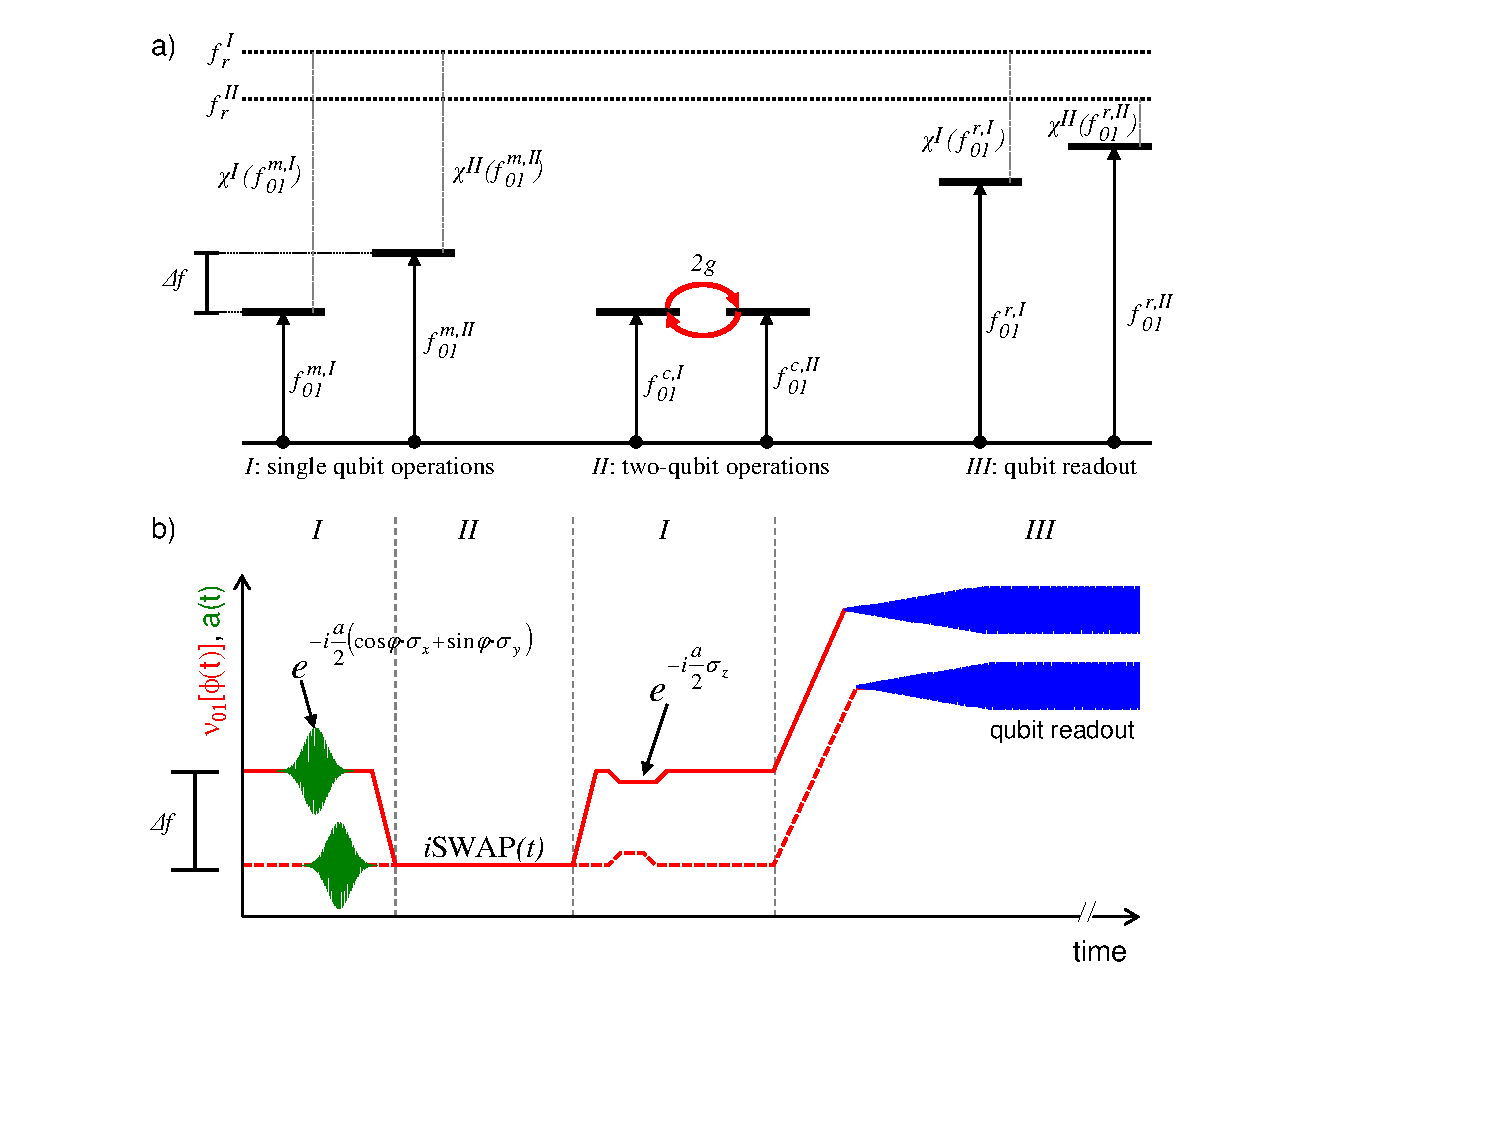
\includegraphics[width=\textwidth]{./material/figures/2-qubit-processor/processor_working_principle}
	\caption[...]{Operation principle of the two-qubit processor. a) The qubit frequencies for different operations. I: Single-qubit manipulation and parking. II: Two-qubit coupling. III: Qubit readout. For each operation, different qubit frequencies are chosen, resulting in different qubit-qubit coupling and qubit-readout couplings $\chi_r^{I,II}(f_{01}^{I,II}$. b) Typical gate sequence illustrating the different operations. The sequence consists of two single-qubit XY-gates, a two-qubit $i\mathrm{SWAP}(t)$ gate, two single-qubit Z-gates and ends with the qubit readout.}
	\label{fig:processor_operation}
\end{figure}

We want to perform three basic operations with the quantum processor:

\begin{itemize}
\item \textbf{Single-qubit gates}: Manipulating a single qubit by rotating its Bloch vector around the $X$, $Y$ or $Z$ axis of the Bloch sphere.
\item \textbf{Two-qubit gate}: Performing a (universal) two-qubit gate, in this work in particular the $\sqrt{i\mathrm{SWAP}}$ and $i\mathrm{SWAP}$ gates.
\item \textbf{Qubit readout}: Performing single-shot readout of the state of each qubit, possibly simultaneously for both of them.
\end{itemize}

The parameter requirements for each of these operations are usually conflicting: For single-qubit manipulation, no interaction between the qubits must be present, hence the qubit frequencies need to be strongly detuned. However, to implement the two-qubit gates, strong resonant interaction between the qubits is required, hence the two qubit frequencies should be resonant. Furthermore, during qubit manipulation the relaxation of the qubit state through the readout resonator should be negligible, hence the frequency detuning $\Delta$ between each qubit and its readout resonator should be large, as shown by eq. (\ref{eq:purcell_rate}). On the other hand, to obtain a high state fidelity during the readout of the qubit state, the interaction between the qubit and its readout resonator should be large, which requires a small frequency detuning $\Delta$ between the two.

\smallskip

We solve these conflicting requirements by dynamically changing the qubit frequencies during the operation of the processor using fast on-chip flux lines. Fig. \ref{fig:processor_operation} illustrates this basic operating principle of the two-qubit processor: For each of the three basic operations (single-qubit manipulation, two-qubit gate and readout), we choose a different set of qubit frequencies $f_{01}^{I,II}$. For the single-qubit gates, the two frequencies $f_{01}^{m,I}$ and $f_{01}^{m,II}$ are detuned by $\Delta f_m = f_{01}^{m,II}-f_{01}^{m,I}$. This tuning is chosen such that only negligible qubit-qubit interaction is present when performing single-qubit manipulations or no operation. Furthermore, at this working point the detuning between each qubit and its readout resonator is such that the qubit lifetime is not limited by relaxation through the gate circuit. To realize a two qubit gate, the two qubits get tuned in resonance such that $f_{01}^{c,I} = f_{01}^{c,II}$. At this point, the qubits experience a swapping interaction as given by eq. (\ref{eq:cqed_qubit_interaction_hamiltonian}) with an effective swapping frequency $2g$. For the readout, we change the qubit frequencies to $f_{01}^{r,I}$, $f_{01}^{r,II}$, reducing the qubit-resonator detuning such that the corresponding dispersive shift $\chi^I(f_{01}^{r,I})$ and $\chi^{II}(f_{01}^{r,II})$ of the resonator during readout assures an optimal readout fidelity. The displacement of the qubit frequency between the different working points has to be performed on a time scale faster than all relevant qubit manipulation and coupling frequencies but not as a fast as to induce transitions of the qubit state.

\smallskip

We discuss now the parameters of each component of the processor in greater detail, explaining each time the relevant design goals and possible conflicts and presenting the parameter choice or compromise we arrive at.

\section{Qubit Design}

The main design goals for the qubits are large coherence times, good frequency tunability and the possibility of fast single-qubit driving. Good frequency tunability is important since we need to move the qubits to different frequency working points for single-qubit and two-qubit manipulation as well as qubit readout. The maximum qubit drive frequency should be large compared to the decoherences times of the qubit, so that we are able to perform a large number of gate operations on the qubit before its coherence is destroyed, which is crucial when running quantum algorithms.

\subsection{Qubit Frequency \& Junction Asymmetry}

The choice of the maximum qubit frequency is influenced by several requirements:

\begin{itemize}
\item The density of thermal photons at the qubit frequency should be sufficiently low at the operating temperature of the circuit (typically 20-100 mK) such that the thermal excitation of the qubit into higher energy levels is negligible.
\item Robust equipment for signal generation and measurement in the frequency range of the qubit should be available. This includes microwave sources needed to generate the charge drive pulses as well as room-temperate and cryogenic microwave components such as mixers, splitters, circulators and amplifiers.
\item The design of microwave circuits is all the more easy, the lower the required frequency range.
\end{itemize}

In addition, the choice of the qubit frequency also influences the choice of the readout resonator frequency. For our qubits, we choose a minimum transition frequency of $\omega_{01}^{1,2}/2\pi= 4 \;\mathrm{GHz}$, which ideally yields a negligible excited state occupation probability of $p(\ket{1})=1/[1+\exp{(\hbar \omega / k_B T)}]=2.1\%$ at $T=50\;\mathrm{mK}$. In addition, in the frequency range $2-18\;\mathrm{GHz}$, commercial microwave equipment and components are available for both room-temperature as well as cryogenic applications. A qubit frequency tunability bandwidth of 3 GHz being sufficient for the operation of the processor, we choose a maximum qubit frequency $\omega_{01}^{max}/2\pi = 7\;\mathrm{GHz}$.

\smallskip

As described in chapter \ref{chapter:theory}, we use a split Josephson junction geometry as shown in fig. \ref{fig:cpb_circuit}b to make the Josephson energy of the qubit tunable by an external flux $\Phi_{ext}$. The modulation depth of $E_J(\Phi_{ext})$ is given by eq. (\ref{eq:josephson_energy_modulation}): The higher the junction asymmetry $d$, the smaller the modulation depth of the Josephson energy $\simeq 1-d$. In general, it can be advantageous to operate the qubit at a working point where $\partial E_J(\Phi)/\partial \Phi=0$ since at that point the qubit will be insensitive to flux noise at first order. Hence we chose an asymmetry $d\approx 0.35$ so that the minimum qubit frequency coincides with our lower boundary frequency of $4\;\mathrm{GHz}$.

\subsection{Single-Qubit Gates} \label{section:qubit_driving}

We distinguish between single-qubit rotations around the $X$ and $Y$ axes and around the $Z$ axis of the Bloch sphere. The latter are implemented by changing the qubit frequency using a fast on-chip flux line, whereas the former are implemented by driving the qubit with an oscillatory electrical drive signal at its resonance frequency. For the $X/Y$ gates, it is necessary to capacitively couple the qubit to an external charge driving circuit. 

\paragraph{Charge Driving} \label{section:charge_driving}

The maximum drive frequency of the qubit is limited by its anharmonicity: Since the Transmon qubit is only weakly anharmonic, when driving the qubit at a frequency comparable to the qubit anharmonicity, transitions to higher Transmon levels will be induced, therefore producing a leakage of the qubit state out of the computational basis and hence unitary drive errors. This effect can be partially alleviated by increasing the anharmonicity of the qubit. However, by increasing the anharmonicity, one also increases the sensitivity of the qubit to charge noise. Hence it is necessary to find a compromise for the value of the qubit anharmonicity which allows sufficiently fast qubit driving but which does not incur too much dephasing.

\smallskip

To estimate the drive error arising due to the finite anharmonicity of a Transmon, we model its driving using a simple three-level Hamiltonian in the rotating-frame, as used e.g. in \cite{motzoi_simple_2009}:
%
\begin{equation}
\hat{H} = \alpha\left(
						 \begin{array}{ccc}
						0 & \epsilon^*(t)/\alpha & 0 \\
						\epsilon(t)/\alpha & \delta/\alpha & \sqrt{2}\epsilon^*(t)/\alpha \\
						0 & \sqrt{2}\epsilon(t)/\alpha & 2\delta/\alpha + 1
						\end{array}
					\right) \label{eq:qubit_three_level_driving_hamiltonian}
\end{equation}
%

Here, $\epsilon(t) = \epsilon_x(t)+i\epsilon_y(t)$ is the complex drive IQ amplitude in the rotating qubit frame, $\delta$ is the detuning of the microwave drive from the Transmon $\omega_{01}$ transition frequency and $\alpha$ is the Transmon anharmonicity. Due to the presence of the third energy level, the effective $\ket{0}\to\ket{1}$ transition frequency will get shifted with respect to the bare frequency $\omega_{01}$ when driving the qubit. For $\delta = \alpha = 0$, the characteristic polynomial of $\hat{H}$ is given as $E(E^2-3|\epsilon|^2/4) = 0$ with the two eigenvalues $E=\pm |\epsilon|\sqrt{3}/2$. Thus, for weak anharmonicities this frequency shift is given approximately as $\Delta_{ac}=\sqrt{3}|\epsilon|/2$. To estimate the leakage to the Transmon level $\ket{2}$ when driving the system, we calculate the eigenvalues and eigenvectors of the Hamiltonian (\ref{eq:qubit_three_level_driving_hamiltonian}). We then decompose an initial state $\ket{0}$ in the basis of eigenstates of $\hat{H}$ and calculate its evolution operator $U_d(t,\delta,\epsilon_0)$ under a constant drive amplitude $\epsilon_0$. By numerically maximizing the occupation probability of the state $\ket{1}$ as a function of the evolution time $t$ and the drive detuning $\delta$ we obtain the ideal gate time, gate error and frequency shift for a $\pi$-pulse at a given drive frequency/anharmonicity ratio. In fig. \ref{fig:three_level_driving_errors} we show these quantities as a function of $\epsilon/\alpha$. As can be seen, the gate error due to leakage into the level $\ket{2}$ increases with the drive frequency. For very large drive frequencies, the gate fidelity saturates at a value of $F\approx 0.86$ (the numerically obtained maximum $\pi$-pulse fidelity for ultra-strong driving of the three-level system is $F_{max}\approx 0.895$). We can make use of fig. \ref{fig:three_level_driving_errors} to estimate the minimum required qubit anharmonicity given the desired gate fidelity and gate time. If we demand a maximum Rabi frequency $\epsilon/2=\Omega_{Rabi}^{max}=2\pi\cdot 100\;\mathrm{MHz}$, which corresponds to a gate time for a single-qubit $\pi$-pulse of $T_\pi=5\;\mathrm{ns}$ small compared to the targeted relaxation and dephasing times of the qubit of $T_1,T_\phi\simeq 1\;\mathrm{\mu s}$, and a maximum $\pi$-gate error of $1-F_\pi = 0.04$, we need an absolute anharmonicity $\alpha > 250\;\mathrm{MHz}$.

\smallskip

It is possible to correct leakage errors using optimized DRAG drive pulses \cite{lucero_reduced_2010,chow_optimized_2010}, thereby eliminating leakage to the third qubit level. In this work, we did not use such techniques but we will  include possible errors arising due to this leakage to higher Transmon levels in our error models when discussing experimental data.

\begin{figure}[htp!]
	\centering
	\includegraphics[width=\textwidth]{"./material/mathematica/three_level_driving_errors"}
	\caption[Single-qubit $\pi$-pulse gate time, gate fidelity and AC stark detuning as a function of drive strength]{The single-qubit $\pi$-pulse gate time, gate fidelity and AC Stark detuning, plotted as a function of the reduced drive strength $\epsilon/\alpha$ applied to the three-level Transmon. As the drive strength increases, the gate time decreases as $\alpha/\epsilon$ whereas the gate fidelity decreases non-monotonously.}
	\label{fig:three_level_driving_errors}
\end{figure}

\smallskip 

Furthermore, charge driving of the qubit is done through the readout resonator on the chip, as shown in fig. \ref{fig:2_qubit_chip_circuit_diagram}. The Rabi frequency of the qubit in eq. (\ref{eq:drive_hamiltonian}) is given as $\Omega_{Rabi}= 2 \beta e V_d \bra{0}\hat{n}\ket{1}$, where the drive voltage $V_d$ seen at the qubit gate capacitance depends on the input voltage $V_{in}$ at the input capacitance of the resonator as given by eq. (\ref{eq:qubit_drive_voltage}). Since the resonator acts as a band-pass filter for the input drive signal, the more the drive frequency $\omega_d$ is detuned from the resonator frequency $\omega_r$, the smaller the gate voltage seen by the qubit is. A Rabi frequency of $\Omega_{Rabi}^{max}/2\pi=100\;\mathrm{MHz}$ at $\omega_{01}/2\pi=4\;\mathrm{GHz}$ corresponds to $V_{in}=0.4\;\mathrm{mV}$ for the resonator parameters that we will choose below, $\omega_r/2\pi = 6.7\;\mathrm{GHz}$, $g_{01}/2\pi=50\;\mathrm{MHz}$ and $Q=800$. With 70 dB attenuation inside the cryostat this corresponds to an input power of $P\approx 15\;\mathrm{dBm}$ at room temperature, which is compatible with our microwave setup.

\paragraph{Flux Driving}

To rapidly change the flux in the qubit loop, we couple each qubit inductively to a fast flux line. The flux induced in the qubit loop by this line is given as $\Phi_{ext}=M I_{fl}$, where $I_{fl}$ is the current in the line and $M$ is the mutual inductance between the flux line and the qubit loop, which can be estimated as $M=\mu_0 l \ln{\left[(d_f+w)/d\right]}/2\pi$, where $l$ is the length of the qubit loop parallel to the flux line, $d_f$ the distance of the loop to the line and $w$ the width of the qubit loop perpendicular to the flux line. In order to avoid sample heating through the flux line, we demand a maximum current for inducing one flux quantum $\Phi_0$ in the loop not in excess of $I_{\Phi_0}^{max}=10\;\mathrm{mA}$, corresponding to an electrical input power of $P^{max}_{in}=50\;\mathrm{mW}$ on a $50 \; \Omega$ transmission line with 20 dB attenuation and $P^{max}_{out}=500\;\mathrm{\mu W}$ on the output transmission line, which can be easily dissipated on the 1 K stage of the cryostat. This yields a minimal value of the mutual inductance $M\ge 0.23\;\mathrm{pH}$, which can easily be achieved with a qubit loop of $l=w=4\;\mathrm{\mu m}$ at a distance $d_f=12\;\mathrm{\mu m}$ to the flux line. The coupling of the qubit to the flux line also induces decoherence that we will take into account later when confirming our choice of $M$.

\smallskip

In general, when passing a low-frequency or DC current through the flux line, superconducting shielding currents will build up in the ground plane around the line. Therefore, we usually remove the ground plane between the center pin of the flux line and the qubit loop, since otherwise the induced shielding currents will modify the effective flux seen by the qubit and lead to unwanted distortions in the shape of the applied flux signal. However, removing this ground plane also leads to stronger capacitive coupling of the qubit to the flux line, thereby increasing qubit relaxation, which we also have to take into account.

\subsection{Qubit-Qubit Coupling} \label{section:qubit_qubit_coupling}

\begin{SCfigure}[1.0][hbt!]
	\centering
	\begin{tabular}{l}
	a) \\ 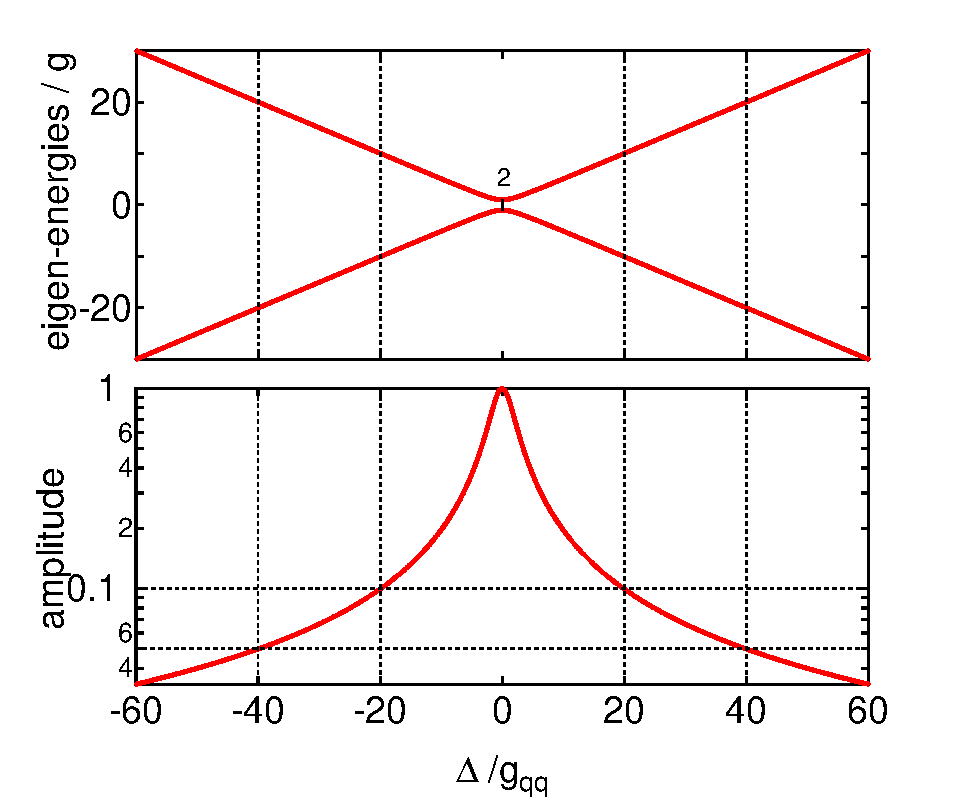
\includegraphics[width=0.49\textwidth]{./material/mathematica/qubit_qubit_coupling} \\
	b) \\ 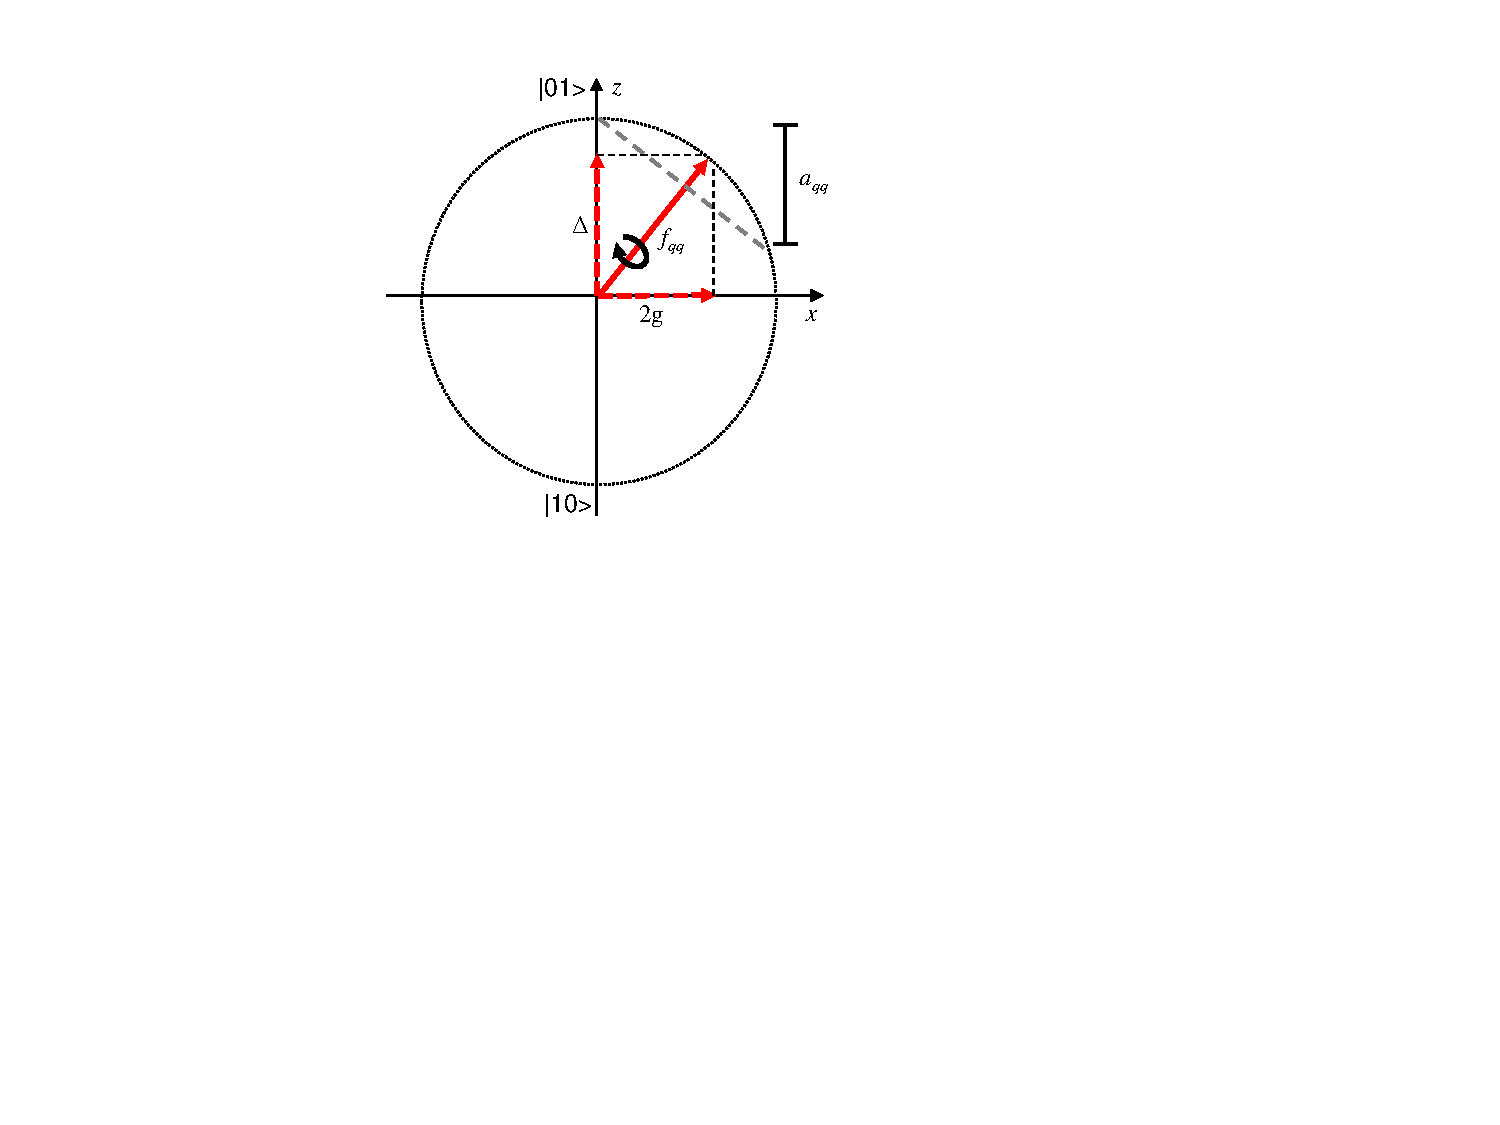
\includegraphics[width=0.49\textwidth]{./material/figures/introduction/bloch_sphere_coupling_illustration}
	\end{tabular}
	\caption[]{a) The two-qubit eigen-energies $E_\pm$ and swapping amplitude $a_{qq}$ as given by eqs. (\ref{eq:qubit_coupling_amplitude_and_frequency}). For $\Delta \gg g$, the amplitude of the swap decreases $\propto 1/\Delta$ and the frequency increases $\propto \Delta$. To effectively switch of the swapping interaction to $a_{qq}=0.1$, a detuning of $\Delta = 20 g$ is required. b) Illustration of the swapping amplitude and frequency on the $\ket{01}$,$\ket{10}$ Bloch sphere: The rotation axis depends on the ratio $\Delta/g$, for $\Delta=0$ it coincides with the $x$ axis whereas for $\Delta \gg g$ it asymptotically approaches the z axis. At the same time, the frequency of rotation around this axis increases $\propto \Delta$. }
	\label{fig:qubit_coupling_amplitude_and_frequency}
\end{SCfigure}

We use a direct capacitive coupling between our qubits to create an interaction between them suitable to implement a two-qubit gate. The full interaction Hamiltonian is given by eq. (\ref{eq:swap_with_detuning}), and the coupling strength $g_{qq}$ between the two qubits can be calculated with eq. (\ref{eq:cqed_capacitive_coupling}). This coupling strength must be chosen such that the interaction between the qubits is sufficiently fast to realize two-qubit gate operations with adequate fidelity, but not too strong in order to still allow to sufficiently suppress the coupling by detuning the qubit frequencies, as needed. By diagonalizing the Hamiltonian (\ref{eq:cqed_qubit_interaction_hamiltonian}) we find for the eigen-energies $E_{qq}^\pm$, the swapping frequency $f_{qq}$ and the swap amplitude $a_{qq}$ of the two coupled qubits as a function of the qubit-qubit detuning $\Delta/2\pi=f_{01}^I-f_{01}^{II}$ the values
%
\begin{eqnarray}
E_{qq}^\pm & = & \pm\frac{1}{2}\sqrt{4g_{qq}^2+\Delta^2}, \notag \\
f_{qq}     & = & \sqrt{4g_{qq}^2+\Delta^2}, \notag \\
a_{qq}     & = & \frac{2g_{qq}}{\sqrt{4g_{qq}^2+\Delta^2}}. \label{eq:qubit_coupling_amplitude_and_frequency}
\end{eqnarray}
%
Figure \ref{fig:qubit_coupling_amplitude_and_frequency} shows the the eigen energies and qubit-qubit swapping amplitude as a function of the normalized qubit-qubit detuning $\Delta/g$. As can be seen, for $\Delta \gg g$ the swap amplitude decreases $\propto 1/\Delta$ whereas the swap frequency increases $\propto \Delta$. For our processor, we demand that the residual swapping amplitude $a\le 0.1$ when the qubits are ``parked'' for single-qubit gates and readout, hence it is necessary to detune the qubits by $\Delta \approx 20 g$. At this detuning, the swapping frequency is given as $f_{qq}(20 g)\approx 20 g$. For our processor, we choose $2g/2\pi = 10\;\mathrm{MHz}$, corresponding to a qubit-qubit detuning of $200\;\mathrm{MHz}$ at $a_{qq}=0.1$ and an associated swapping frequency $f_{qq}=100\;\mathrm{MHz}=(10\;\mathrm{ns})^{-1}$. The required frequency displacement is easily achievable with the on-chip fast flux lines. On resonance, the swap frequency of $10\;\mathrm{MHz}$ allows us to realize an $\sqrt{i\mathrm{SWAP}}$ gate in $25\;\mathrm{ns}$ and an $i\mathrm{SWAP}$ gate in $50\;\mathrm{ns}$, which is sufficiently fast compared to the estimated relaxation and dephasing times of the qubits. The residual swapping between the qubits at their parking position is usually small enough to be irrelevant for most experiments performed in this work. However, when executing long gate sequences, as required for certain algorithms, the induced error may be too large, hence a larger detuning should be chosen for these cases.

\smallskip

To estimate the error due to finite rise times for the flux pulse before the $i\mathrm{SWAP}$ gate, we numerically solve the Schrödinger equation of the 2-qubit system in the $\ket{01},\ket{10}$ basis, which is given as
%
\begin{equation}
i\hbar\left(\begin{array}{c} \dot{\psi}_{01} \\ \dot{\psi}_{10} \end{array}\right) = \left( \begin{array}{cc} -\frac{\Delta(t)}{2} & g \\ g & \frac{\Delta(t)}{2}  \end{array} \right)\cdot \left(\begin{array}{c} \psi_{01} \\ \psi_{10} \end{array}\right) \label{eq:swap_evolution}
\end{equation}
%

\begin{figure}[ht!]
\def\imagetop#1{\vtop{\null\hbox{#1}}}

	\centering
	\begin{tabular}{ll}
	a) & b) \\
	\imagetop{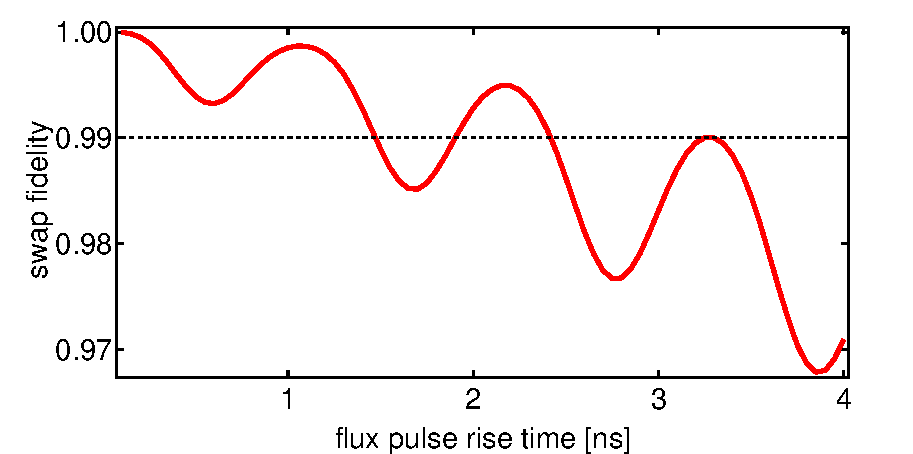
\includegraphics[width=0.6\textwidth]{./material/mathematica/qubit_qubit_swap_error}} &
	\imagetop{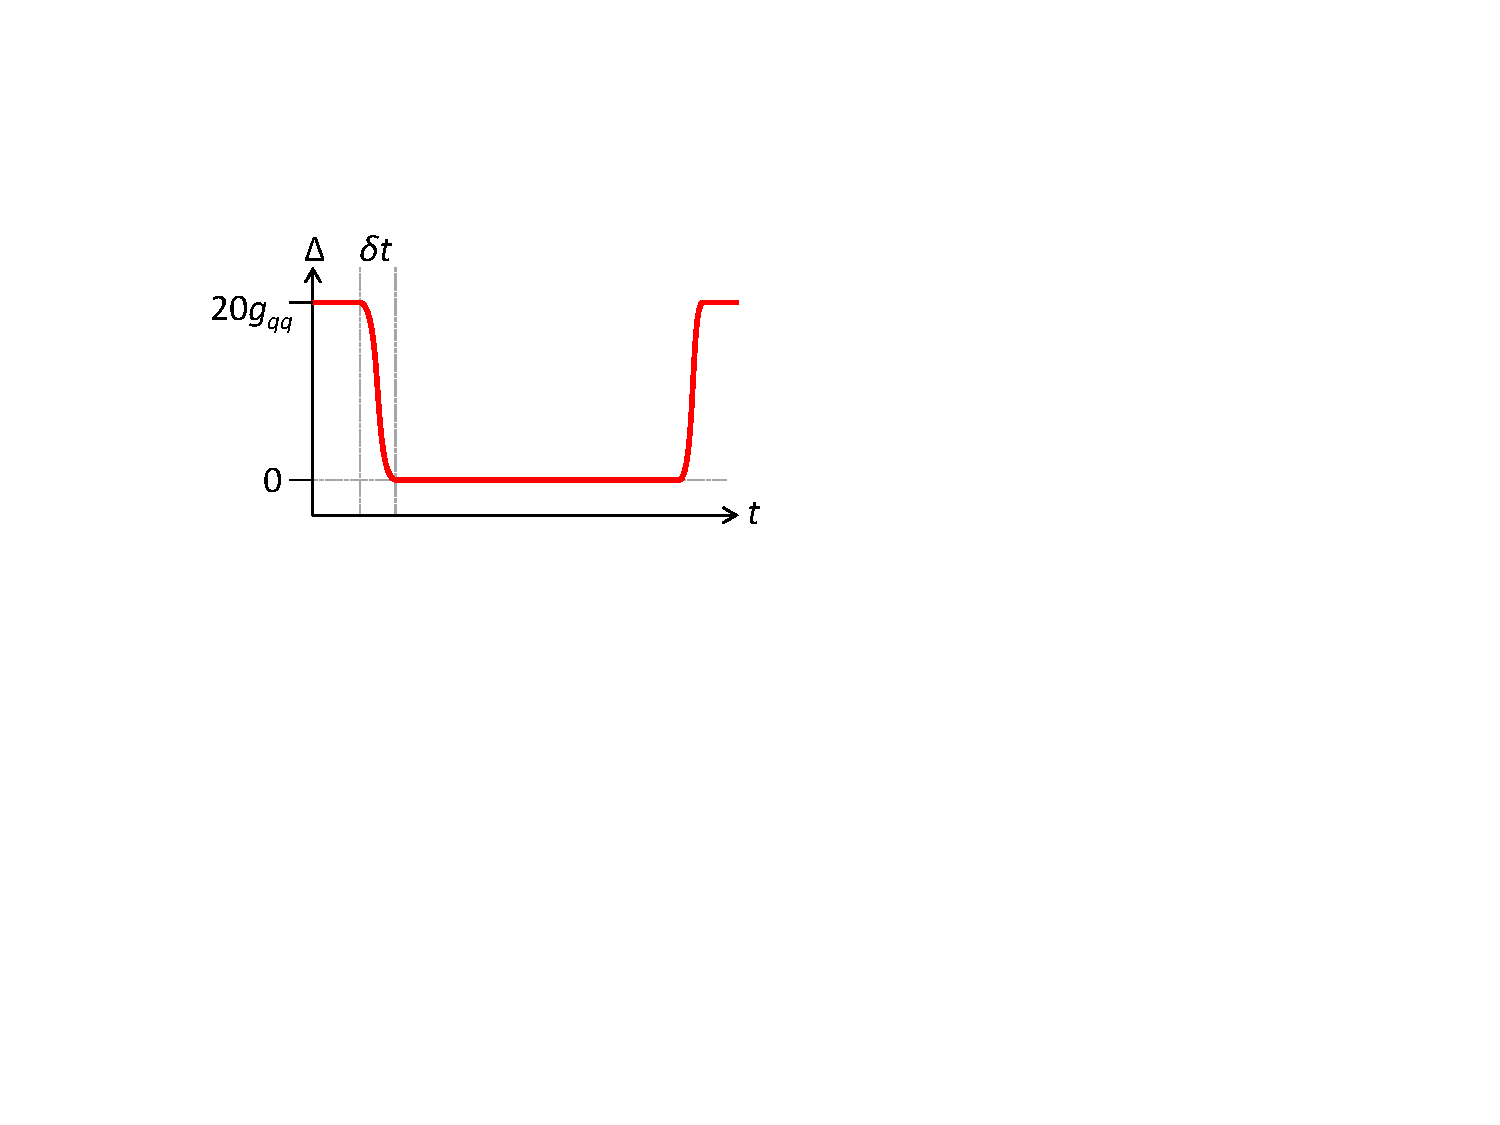
\includegraphics[width=0.4\textwidth]{./material/figures/2-qubit-processor/flux_pulse_rise_time}}
	\end{tabular}
	\caption[]{a) Numerically obtained maximum fidelity of a two-qubit $i\mathrm{SWAP}$ gate realized by changing the detuning $\Delta$ in eq. (\ref{eq:swap_evolution}) from $\Delta = 20g$ to $\Delta=0$ using a Gaussian pulse of width $\delta t$. b) Simulated pulse shape used to obtain the curve shown.}
	\label{fig:qubit_qubit_coupling_swap_error}
\end{figure}

To estimate the error, we go from a detuning $\Delta = 20 g$ at $t=0$ to a detuning $\Delta=0$ using a Gaussian waveform with a rise time $\delta t$. We then numerically determine the maximum SWAP amplitude between the qubits and plot the resulting value against $\delta t$. The result of this simulation is shown in fig. \ref{fig:qubit_qubit_coupling_swap_error}. As can be seen, the fidelity of the gate decreases in a non-monotonous way as a function of the flux pulse rise time. In order to obtain $F>0.99$, a flux pulse rise time of $\delta t \le 1.5\;\mathrm{ns}$ is required.

\subsection{Relaxation and Dephasing}

In this section we discuss the relaxation and dephasing channels of the Transmon qubit which are most relevant to our experiment. We analyze the relaxation and dephasing rates as a function of the Transmon parameters and optimize these parameters to achieve maximum qubit coherence times.

\begin{SCfigure}[1.0][ht!]
	\centering
	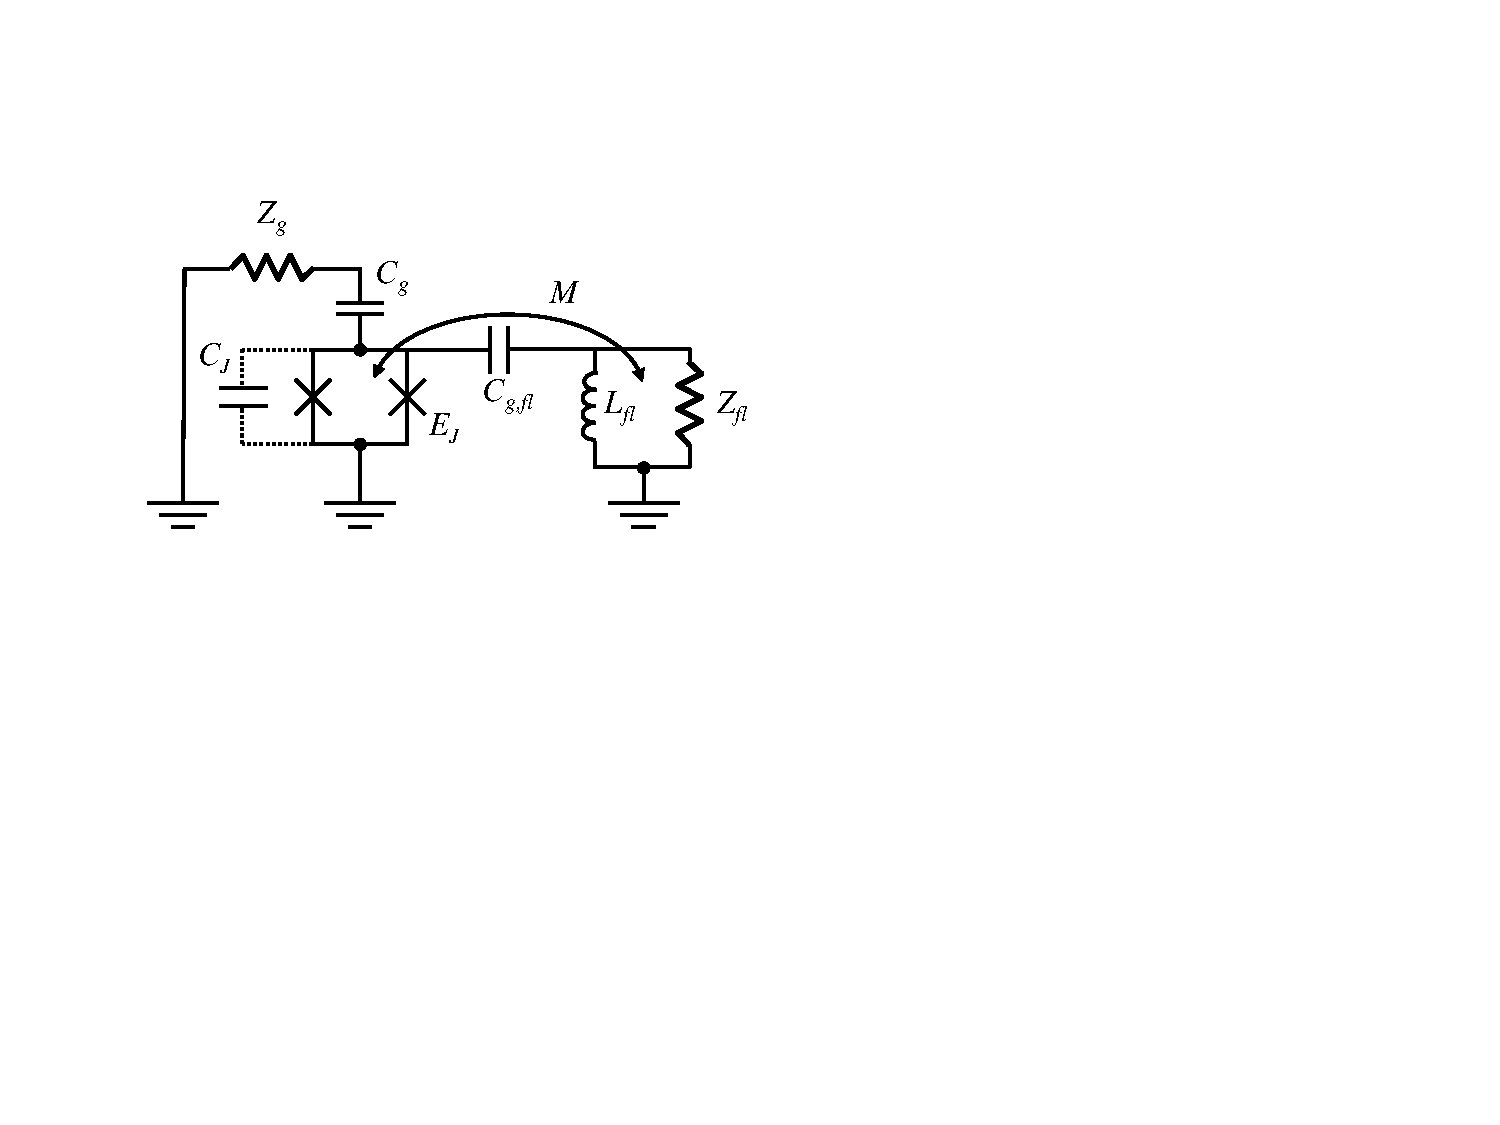
\includegraphics[width=0.6\textwidth]{./material/figures/introduction/cooper_pair_box_decoherence}
	\caption[]{A schematic model showing the coupling of the qubit to its environment, modeled by impedances $Z_g$ and $Z_{fl}$, through capacitive and inductive couplings $C_g$ and $M$.}
	\label{fig:cooper_pair_box_decoherence}
\end{SCfigure}

\subsubsection{Qubit Relaxation}

Relaxation of the qubit can occur either through the charge channel or the flux channel. The qubit has a capacitive coupling to both the flux line and the readout resonator, hence charge relaxation through both of them is possible. On the other hand, the only relevant relaxation channel through the flux channel is through the inductive coupling to the external flux line.

\paragraph{Relaxation through the Gate Charge Channel}

Since the CPB is coupled to an external impedance (in this case the readout resonator that is coupled to a lossy input transmission line) through a gate capacitance $C_g$, as shown in fig. \ref{fig:cooper_pair_box_decoherence}, relaxation into modes of the input impedance seen by the qubit can occur. The relaxation time of the Transmon qubits used in previous experiments was found to be limited to $T_1^{int}=1-4\;\mathrm{\mu s}$ independent of the circuit \citep{simmonds_decoherence_2004,martinis_decoherence_2005}. Consequently, we require the relaxation time associated to charge relaxation through the gate circuit to be significantly longer than this intrinsic relaxation time, i.e. $\Gamma_1^{Purcell}\ll 1\;\mathrm{MHz}$. This requirement influences the choice of the coupling of the qubit to the readout resonator $g_{01}$, the quality factor and associated loss rate $\kappa$ of this resonator and the qubit-resonator detuning $\Delta$ for the different processor operations. The relaxation rate due to the coupling of the qubit to the input resonator is given by eq. (\ref{eq:purcell_rate}). For the qubit parameters chosen above, a resonator quality factor $Q=800$ and a resonator-qubit coupling of $g_{01}/2\pi=50\;\mathrm{MHz}$ chosen below, the relaxation rate is $\Gamma_1^{Purcell}\approx 0.25\;\mathrm{MHz}$ at $\Delta/2\pi = 2\;\mathrm{GHz}$ (for qubit manipulation) and $\Gamma_1^{Purcell}\approx 1\;\mathrm{MHz}$ at $\Delta/2\pi = 1\;\mathrm{GHz}$ (for qubit readout). This rate is comparable or larger than the typical intrinsic relaxation rate of the qubit and thus compatible with our design goals.

\smallskip

In addition to the capacitive coupling to the input impedance $Z_g$, the qubit is also coupled to its flux line by $C_{g,fl}$, which can lead to relaxation through the charge channel of the flux line \citep{johnson_controlling_2010}. Assuming that the flux line is terminated by a 50 $\Omega$ load and that $C_{g,fl}\le 10\;\mathrm{fF}$. yields a relaxation rate $\Gamma_1^{\mathrm{fl},n_g}\le 260 \;\mathrm{kHz}$ for the qubit parameters discussed above, which is lower than the maximum demanded relaxation rate and thus compatible with our design requirements.
 
\paragraph{Relaxation through the Flux Channel} \label{section:relaxation_through_charge}

On the two-qubit chip, each Transmon is equipped with a fast magnetic flux line that is used to perform flux biasing and fast frequency displacements. The flux lines are coupled to the qubits through a mutual inductance $M$, as shown in fig. \ref{fig:cooper_pair_box_decoherence}. The sensitivity of the qubit to relaxation through the flux channel via the mutual inductance $M$ is given by eq. (\ref{eq:flux_relaxation_sensitivity}). For the mutual inductance discussed above, $M \approx 0.23\;\mathrm{pH}$, a characteristic impedance of the flux line of $Z_{fl}=50\;\Omega$, a qubit frequency $\omega_{01}/2\pi= 7 \;\mathrm{GHz}$ and anharmonicity $\alpha=-250\;\mathrm{MHz}$ and an asymmetry $d=0.35$, we obtain a maximum relaxation rate of $\Gamma_1^{fl}=0.28\;\mathrm{MHz}$, which is small compared to all other relevant relaxation rates. This rate represents an upper bound for an unfiltered flux line, in our experiment the low-pass filtering of the line will further decrease this rate by decreasing $\mathrm{Re}(1/Z_{fl}(\omega_{01}))$ at the qubit frequency $\omega_{01}$. We confirm therefore our choice of the mutual inductance $M=0.25\;\mathrm{pH}$ for the flux coupling of the qubit. 

\subsubsection{Qubit Dephasing}

Dephasing of the qubit can occur due to coupling to external charge or flux noise. Here we will calculate the associated rates for both cases for our designed qubit parameters.

\paragraph{Dephasing through the Flux Channel}

For the qubit parameters discussed in the last paragraph, using eq. (\ref{eq:flux_dephasing_rate}) we obtain a maximum dephasing rate $\Gamma_\phi^{\delta \phi_{ext}}= 0.3\;\mathrm{MHz}$ in the relevant frequency interval $\omega_{01}/2\pi = 4-7 \; \mathrm{GHz}$. This rate is thus smaller than the relaxation-limited dephasing rate of the qubit at all relevant working frequencies of our processor. Our choice of qubit parameters is thus compatible with the demanded dephasing time.

\paragraph{Dephasing through the Charge Channel}

We can use eq. (\ref{eq:charge_dephasing_rate}) to calculate the charge-induced dephasing rate of our Transmon qubit. This rate depends exponentially on the ratio $E_J/E_C$. The highest dephasing rate occurs thus at the smallest qubit frequency that we operate our qubit at, in our case $\omega_{01}/2\pi=4\;\mathrm{GHz}$. The chosen maximum tolerable dephasing rate of $\left(\Gamma_{\phi}^{\delta N_g}\right)^{-1} \approx 1\;\mathrm{\mu s}$ at $\omega_{01}/2\pi=4\;\mathrm{GHz}$ is obtained for a qubit anharmonicity of $\alpha\approx-500\;\mathrm{MHz}$, which is thus the upper bound for the anharmonicity. However, for this work we choose $\alpha=-250\;\mathrm{MHz}$, since it allows already for sufficiently fast driving of the qubit, as discussed in section \ref{section:qubit_driving}. For this parameter choice, we obtain a negligible maximum dephasing rate $\left(\Gamma_{\phi}^{\delta N_g}\right)^{-1} \approx 1\;\mathrm{ms}$ at $\omega_{01}/2\pi=4\;\mathrm{GHz}$. 

\smallskip

As mentioned in section \ref{section:decoherence_in_cqed}, the coupling of the qubit to the readout resonator can induce dephasing trough the AC-Stark shift of the qubit induced by photon-number fluctuations in the resonator. The resulting relaxation rate is given by eq. (\ref{eq:thermal_photon_number_dephasing_rate}). For the qubit parameters discussed above and a qubit-resonator coupling $g_{01}/2\pi=50\;\mathrm{MHz}$, the dephasing rate is $\Gamma_\phi^{\bar{n}}= 0.95\cdot{\bar{n}} \;\mathrm{MHz}$ at the minimum chosen qubit-resonator detuning $\Delta = 1 \;\mathrm{GHz}$. The average number of photons in a resonator with $\omega_{r}/2\pi = 6.7\;\mathrm{GHz}$ at $T=100\;\mathrm{mK}$ is given as $\bar{n} = [\exp{(\hbar\omega_r/k_B T)-1}]^{-1} \approx 0.05$, yielding an effective dephasing rate $\Gamma_\phi^{\bar{n}}\approx 38\;\mathrm{kHz}$, which is small compared to the flux-induced dephasing rate at all working points of the qubit.

\section{Readout Design}

As explained in section \ref{section:jba_operation_principle} of chapter \ref{chapter:theory}, the readout fidelity is influenced by three sources of error: Finite overlap between the switching probability distributions for different qubit states, relaxation of the qubit during the measurement phase of the readout and retrapping of the resonator state during the latching phase of the readout. In order to minimize these errors, the following constraints should be met for the readout resonator:

\begin{enumerate}
\item The state-dependent dispersive shift of the resonator frequency should be large enough such that the switching probability distributions of the resonator corresponding to the qubit states $\ket{0}$ and $\ket{1}$ do not overlap.
\item The measurement phase of the readout should be completed in a time $T_{meas}$ which is short compared to the relaxation time of the qubit, i.e. $T_{meas}\ll T_1$.
\item There should be no retrapping of the resonator state during the latching period of the readout.
\end{enumerate}

In order to maximize the dispersive shift, we can either increase the coupling $g_{01}$ between the resonator and the qubit or reduce the frequency detuning $\Delta$ between them. However, increasing $g_{01}$ or decreasing $\Delta$ will also increase the relaxation rate of the qubit through the Purcell effect, thereby reducing the readout fidelity. There is thus an optimum choice for $g_{01}$ and $\Delta$ \citep{mallet_single-shot_2009}. To counteract the qubit relaxation through the cavity, we can simply increase the quality factor of the resonator. However, usually the maximum relaxation time of the Transmon qubit used in this work is limited to $T_1\approx 1-4\;\mathrm{\mu s}$ due to intrinsic relaxation processes. Therefore, increasing the quality factor of the resonator does not necessarily increase the readout fidelity because a higher quality factor also increases the time required to excite the readout resonator by the drive pulse and hence the measurement time of the qubit state. Therefore, if the qubit relaxation time is intrinsically limited, a longer measurement time at a constant relaxation rate implies a higher probability for the qubit to relax during the measurement, hence actually reducing the readout fidelity. We therefore need to find a compromise for the values of $g_{01}$, $\chi$ and $\Delta$ that will maximize the readout fidelity under the given constraints.

\begin{SCfigure}[1.0][ht!]
	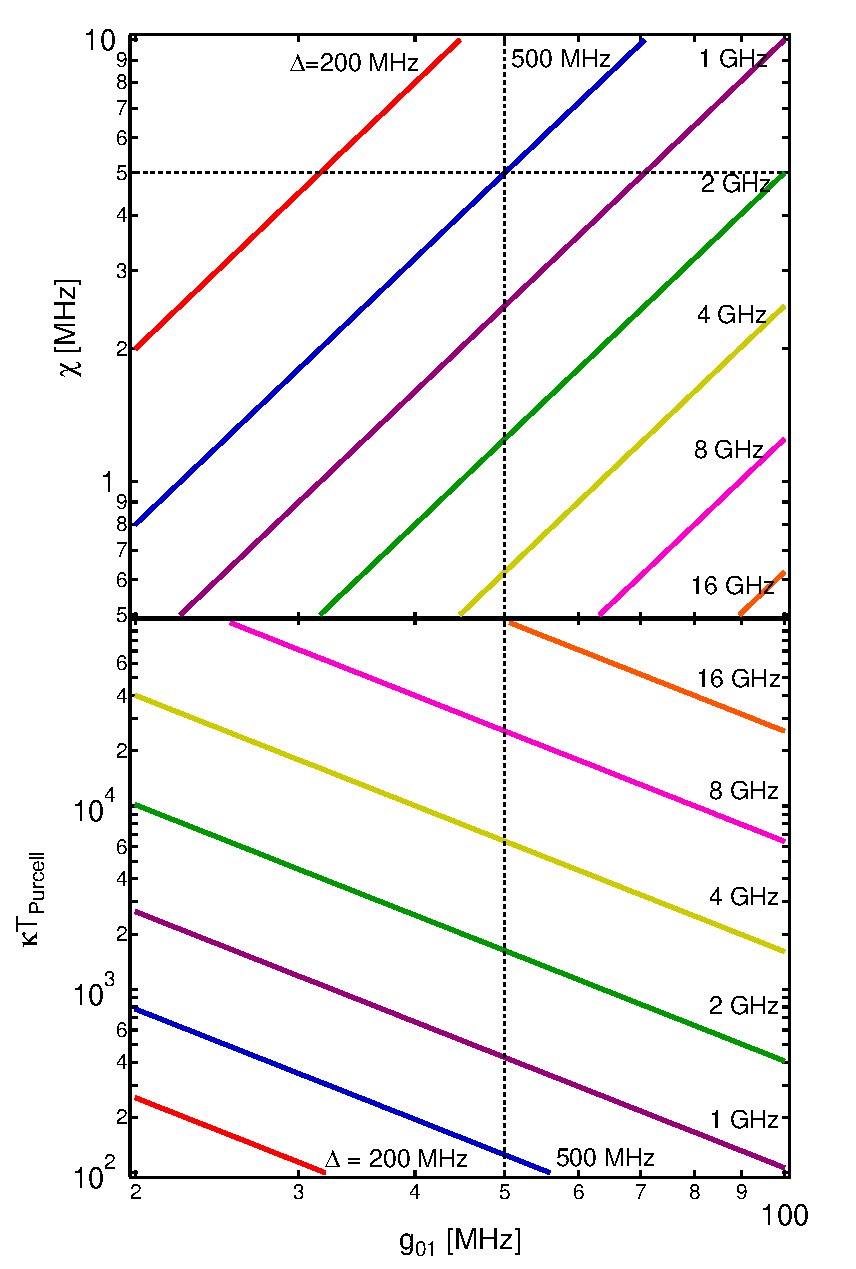
\includegraphics[width=0.6\textwidth]{./material/mathematica/readout_purcell_and_chi_vs_g}
	\caption[]{The dispersive shift $\chi$ of the resonator and the relaxation time $\kappa\cdot T_{Purcell}$ (normalized to the decay rate $\kappa=\omega_r/Q$ of the resonator) of the qubit for a qubit dispersively coupled to a resonator, plotted as a function of the coupling strength $g_{01}$ and shown for different values of the qubit-resonator detuning $\Delta = \omega_{r}-\omega_{01}$.}
	\label{fig:purcell_rate_and_chi}
\end{SCfigure}


To illustrate the effect of $g_{01}$ and $\Delta$ on the relaxation time $T_1$ and the dispersive shift $\chi$, fig. \ref{fig:purcell_rate_and_chi} shows both quantities as a function of $g_{01}$, plotted for several choices of $\Delta$. Now, criterion 1 above demands that the dispersive shift be large enough to completely separate the switching probability distributions for different qubit states. The width of these probability curves can be calculated theoretically, however for this discussion we rely on experimentally measured values and assume that a dispersive shift of $\Delta \chi \approx 5\;\mathrm{MHz}$ suffices to fully separate the two distributions. This assumption limits the range of possible values for $g_{01}$ and $\Delta$ to the region above the horizontal line in fig. \ref{fig:purcell_rate_and_chi}a. On the other hand, criterion 2 demands that the time required to map the qubit state to the oscillator state should be small compared to the relaxation time of the qubit. For the CJBA parameters relevant to this work, this time is given as $T_{meas}\approx 50-100\;\mathrm{ns}$. In order to have negligible qubit relaxation during the readout, we therefore demand that $T_1 \ge 1\;\mathrm{\mu s}$, which corresponds to a 5 \% relaxation probability during the measurement interval. This again limits the choice of possible values of $g_{01}$ and $\Delta$. 

\smallskip

Another important design parameter of the CJBA is the Kerr constant $K$. This constant defines the non-linearity of the resonator and determines the power at which the resonator becomes bistable. Also, the number of photons in the low- and high-amplitude solution of the resonator increases with increasing $K$. Since the dispersive shift of the qubit frequency caused by the resonator is proportional to the number of these photons, choosing a too high $K$ should be avoided since it can induce large displacements of the qubit frequency, thereby recoupling the two qubits of the processor during the readout operation. 

\smallskip

Taking these constraints into account, for the final choice of parameter values we rely on a set of optimized CJBA parameters that have been obtained in an earlier experiment by Mallet {\it et. al.} \citep{mallet_single-shot_2009}. For our processor we choose readout resonator frequencies $\omega_r^1/2\pi = 6.7 \;\mathrm{GHz}$ and $\omega_r^2/2\pi = 6.85\;\mathrm{GHz}$, quality factors $Q^{1,2}=800$, Kerr constants $2\pi K^{1,2}/\omega_r^{1,2}=-2.5\times 10^{-5}$ and qubit-resonator couplings $g_{01}^{1,2}/2\pi=50\;\mathrm{MHz}$. In addition, we choose a detuning $\Delta/2\pi = 500\;\mathrm{MHz}$ for reading out the qubits, yielding a relaxation rate $\Gamma^{Purcell}_1\approx 0.5\;\mathrm{MHZ}$ during readout.

\section{Summary: Qubit and Readout Parameters}

Having discussed the relevant properties of all building blocks of our processor and their dependence on the sample parameters, we choose a full set of these parameters, summarized in table \ref{table:processor_parameters}. The left column contains the processor parameters, the right column the related sample parameters.

\begin{table}
	\centering
	\begin{tabularx}{\textwidth}{r|X|l}
	Parameter & Value & Related Parameters \\ [0.3cm]
	$E_J$ & $h\cdot 28.4\;\mathrm{GHz}$ & $f_{01}=7\;\mathrm{GHz}$, $\alpha=-250\;\mathrm{MHz}$ \\ [0.3cm]
	$E_C$ & $h\cdot 0.92\;\mathrm{GHz}$ & $C_q = 42\;\mathrm{fF}$, $I_c = 57.4 \;\mathrm{nA}$\\ [0.3cm]
	$d$ & $0.35$ & \\ [0.3cm]
	$M_{1,2}$ & $0.25\;\mathrm{pH}$ & \\ [0.3cm]
	$g_{qq}/2\pi$  & $10\;\mathrm{MHz}$ & $C_{qq}=0.45\;\mathrm{fF}$ \\ [0.3cm]
	$g_{01}/2\pi$  & $50\;\mathrm{MHz}$ & $C_{qr}\approx 62.8 \;\mathrm{fF}$ \\ [0.3cm]
	$\omega_r^{1}/2\pi$ & $6.7\;\mathrm{GHz}$ & $L_r^1 = 756\;\mathrm{pH}$, $C_r^1= 497 \;\mathrm{fF}$ \\ [0.3cm]
	$\omega_r^{2}/2\pi$ & $6.85\;\mathrm{GHz}$ & $L_r^2 = 739\;\mathrm{pH}$, $C_r^2= 486 \;\mathrm{pF}$\\ [0.3cm]
	$Q_r^{1,2}$ & $800$ & $C_{in}^{1,2}\approx 17 \;\mathrm{fF}$ \\ [0.3cm]
	$K_r^{1,2}$ & $-2.5\times 10^{-5}$ & $I_{J,r}\approx 2.3 \;\mathrm{\mu A}$ \\ [0.3cm] 
	\end{tabularx}
	\caption[]{The sample parameters chosen for the two-qubit processor. The table contains all independent parameters of the processor as well as the dependent parameters derived from them.}
	\label{table:processor_parameters}
\end{table}

\section{Processor Layout \& Fabrication}

\begin{figure}[ht!]
	\centering
	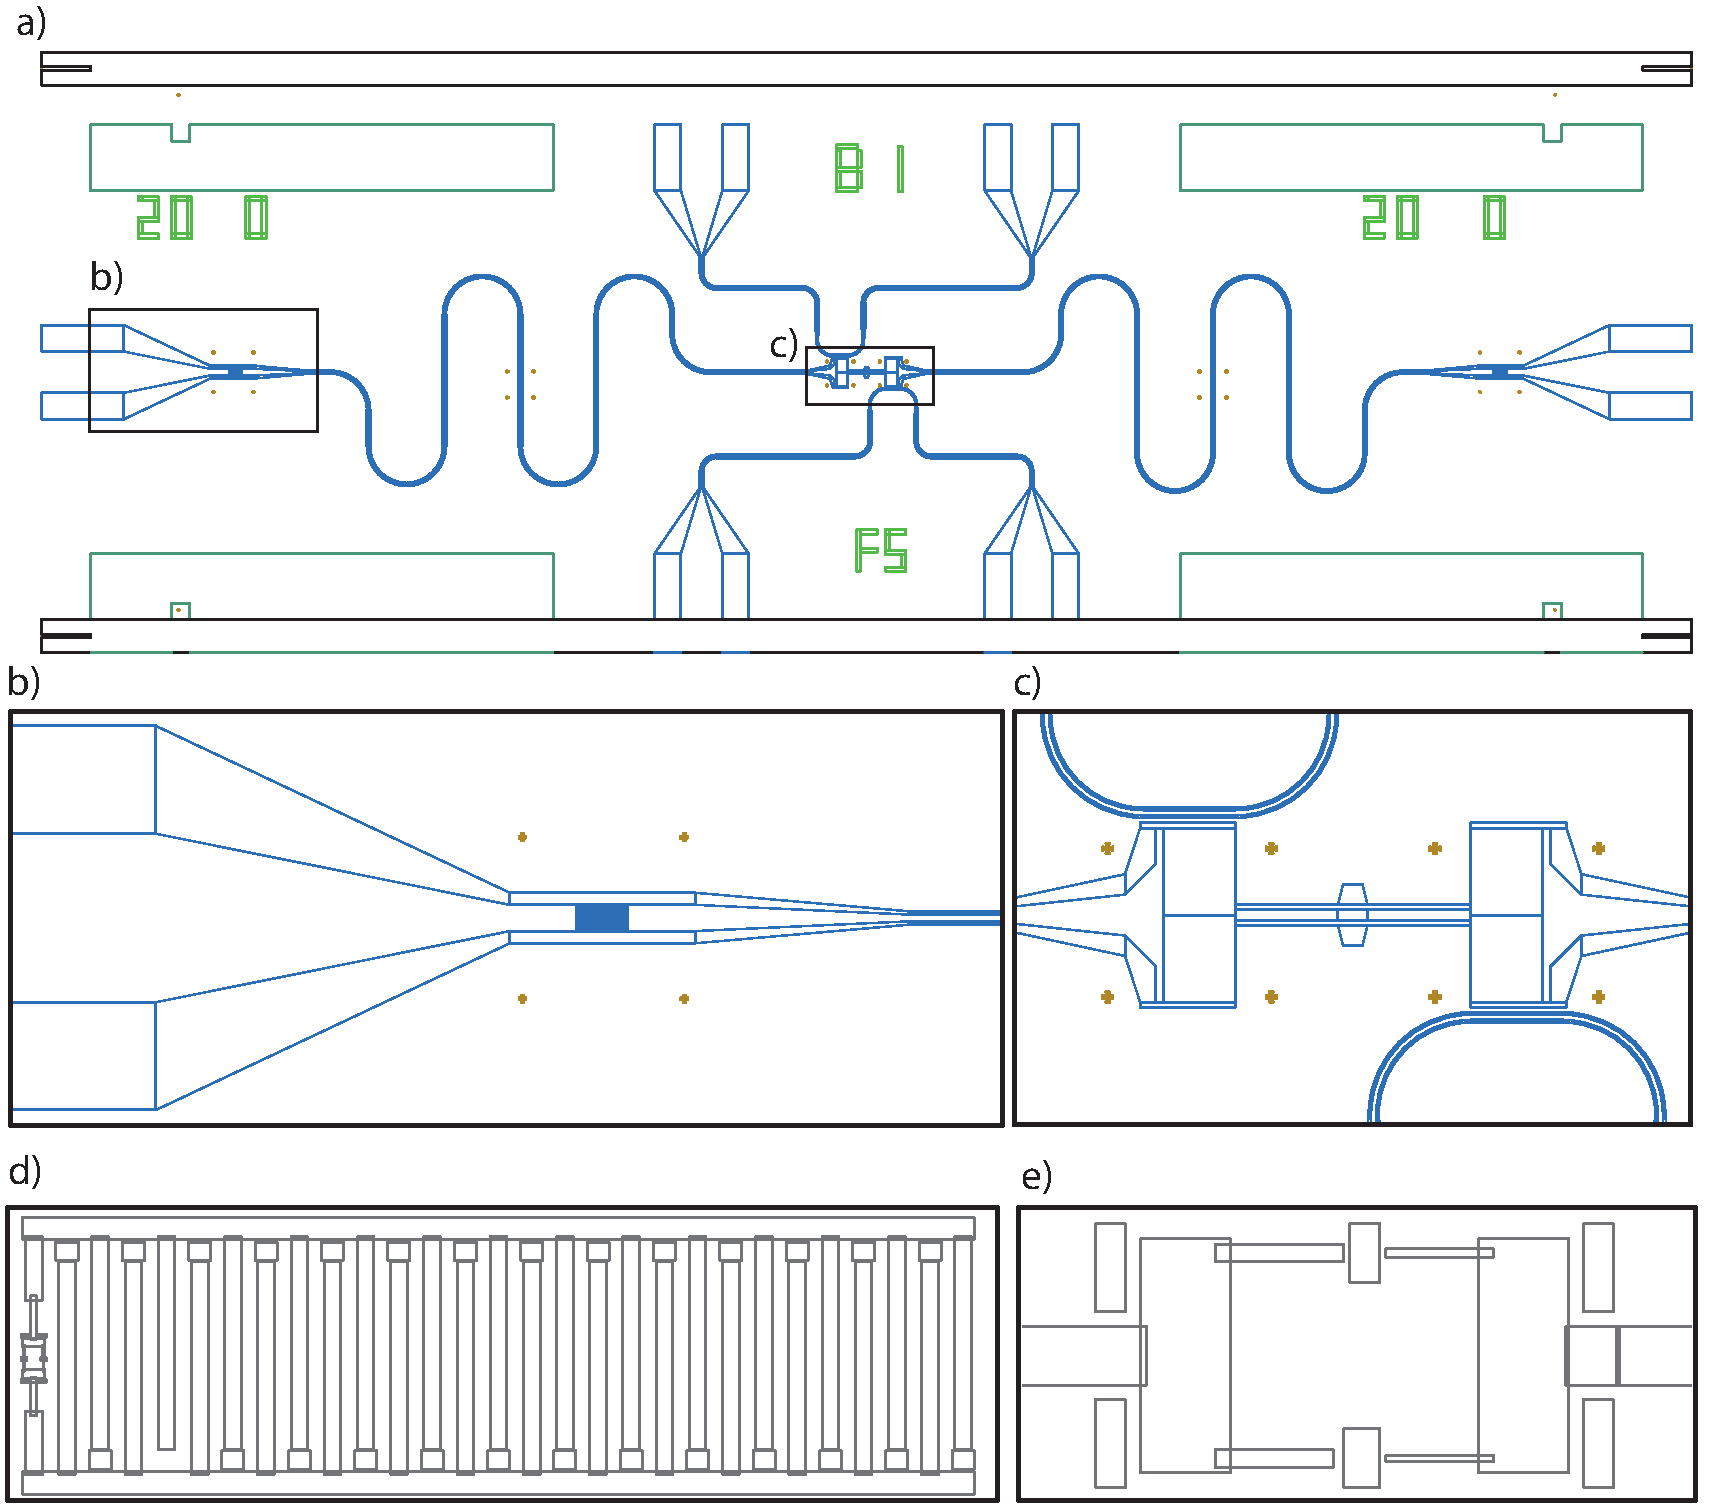
\includegraphics[width=\textwidth]{./material/figures/2-qubit-processor/fabrication/qubit_processor_layout}
	\caption[]{CAD layout schematic of the two-qubit processor, showing the two CPW readout resonators and the two qubits with their adjacent fast flux lines. Sub figures a) and b) show the CAD drawing of the Transmon capacitance and SQUID, as used for the electron beam lithography. Sub figure c) gives a magnified view of the two qubits and their capacitive coupling element, subfigure d) shows the input coupling capacitance of the CPW resonator to the input transmission line.}
	\label{fig:processor_fabrication}
\end{figure}

After having chosen a set of sample parameters, it remains to find a physical implementation of the design that we can realize. In this section we discuss therefore the layout design of the qubit processor. From the beginning, we will restrict our discussion to lithographically fabricated circuits on a chip, disregarding recent approaches to the realization of superconducting qubits and resonators using 3D microwave cavities \citep{paik_observation_2011}.

\smallskip

The readout resonator can be realized as a lumped-elements LC resonator or as a transmission line resonator. In the original approach to CQED \citep{wallraff_strong_2004}, a coplanar waveguide (CPW) resonator was used. Distributed microwave resonators such as CPW resonators are often advantageous since they can be fabricated with a high intrinsic quality factors \citep{megrant_planar_2012,creedon_high_2011,wang_improving_2009,barends_minimal_2010}, although recently large progress has been made concerning the quality factors of discrete LC resonators as well \citep{khalil_loss_2011}. Also, the isolation between the input port of the distributed resonator and the qubit electrode to which the open end of the resonator is coupled is high, whereas for a discrete LC resonator a significant capacitive coupling between the input port of the resonator and the qubit can exist, which is unwanted since it will cause additional relaxation. For this work, we therefore chose a distributed design using a $\lambda/2$ CPW resonator. The open port of the resonator is capacitively coupled to one of the qubit electrodes to achieve the desired coupling factor $g_{01}$.

\smallskip

The flux lines can be realized in several ways. For our processor, we choose a simple 50 $\Omega$ CPW transmission line that is passing nearby the qubit SQUID at a distance of $d\approx 12\;\mathrm{\mu m}$. Since we use the flux line for DC biasing of the qubits as well, shielding currents will flow in the ground planes on either side of the line when a DC current gets applied. These currents can create an unwanted flux bias in the qubit loop and should therefore be eliminated. We achieve this by removing the ground plane between the qubit and the central conductor of the flux line. By doing this, we also increase the capacitive coupling between the line and the qubit electrodes, thereby increasing the charge relaxation rate through the flux line. However, as discussed in section \ref{section:relaxation_through_charge}, for our sample parameters this effect is usually negligible. The flux line can be terminated either directly at the 20 mK stage by wire-bonding it to the ground plane of the chip, or by connecting it to a matched impedance at the 1 K stage of the cryostat. Alternatively, we can also feed back the flux signal to room temperature, which is useful for e.g. measuring the response function of the line.

\smallskip

For the Transmon qubit itself, we need to fabricate a large shunt capacitance $C_J$ in order to achieve the desired charging energy. We implement this capacitance as an interdigitated planar capacitor that we pattern together with the qubit junctions using electron-beam lithography. The Josephson junctions of the qubit are realized in a SQUID geometry with a loop area of $A\approx 16\;\mathrm{\mu m}^2$ and are fabricated using double-angle shadow-evaporation of Aluminium.

\section{Electromagnetic Simulation of the Qubit-Chip}

\begin{figure}[ht!]
	\centering
	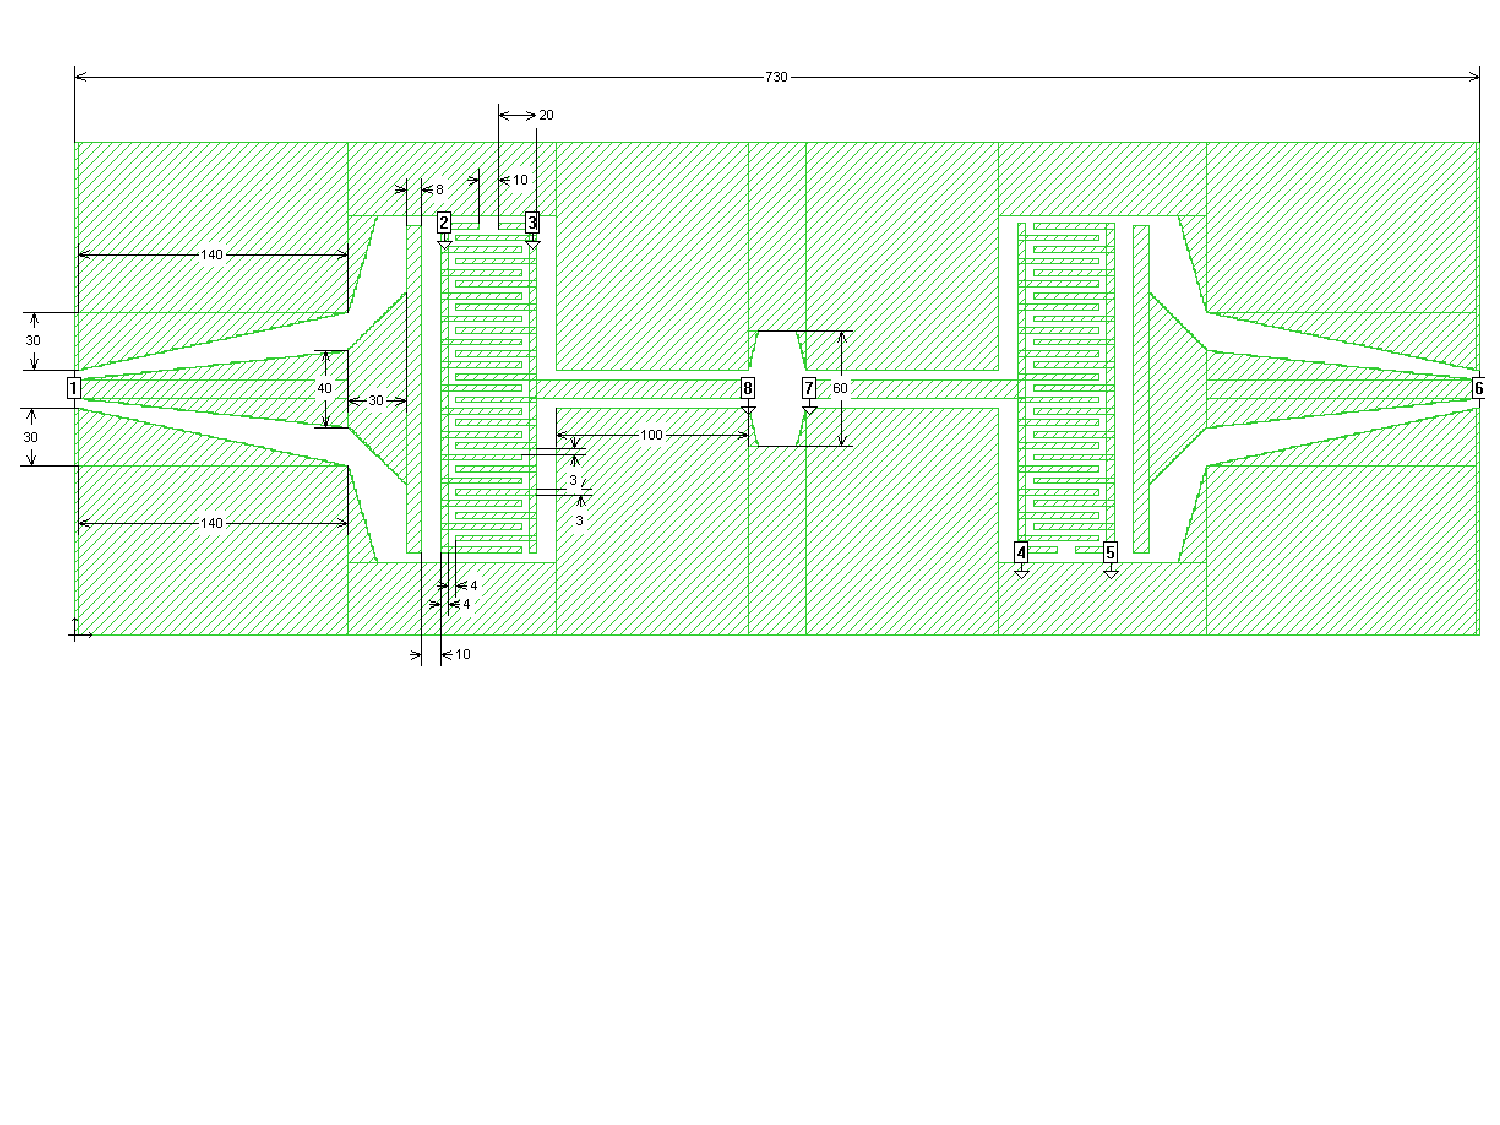
\includegraphics[width=\textwidth]{./material/figures/2-qubit-processor/sonnet_simulation_of_qubit_chip}
	\caption[]{2D model used to model the qubits of the processor using Sonnet microwave simulator (SONNET). Shown are the two Transmon qubit capacitances that are capacitively coupled to each other and to their readout resonator (not shown). Numerical simulation of the circuit yields the capacitances and inductances between all ports of the circuit (1-8).}
	\label{fig:sonnet_model_of_qubit_chip}
\end{figure}

We use a software package for electromagnetic simulation (SONNET) to simulate individual parts of the chip an obtain the transmission coefficients between all relevant circuit components and an equivalent lumped-element model of the circuit. Using this equivalent model we calculate all relevant capacitances and inductances. We can then iteratively adapt the geometry of individual elements in order for them to match the designed parameter values. Fig. \ref{fig:sonnet_generated_model} shows an example of a circuit model generated by this method.

\smallskip

\begin{SCfigure}[1.0][ht!]
	\centering
	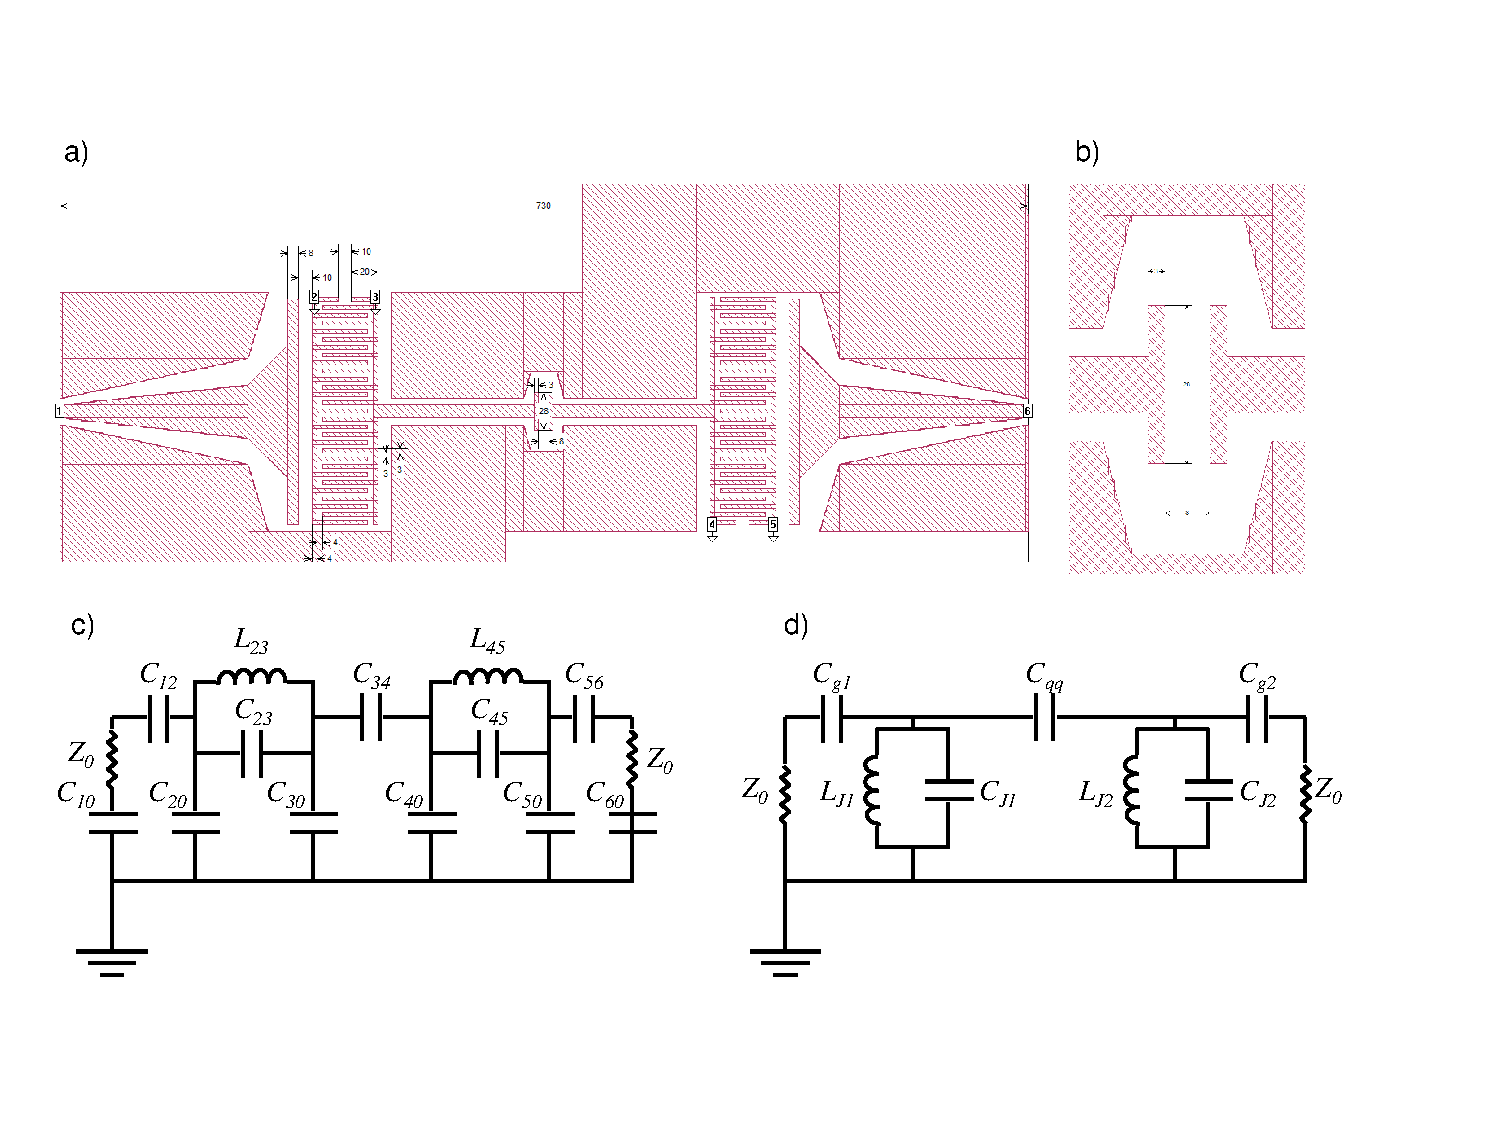
\includegraphics[width=0.6\textwidth]{./material/figures/2-qubit-processor/sonnet_model}
	\caption[]{A circuit model of the geometry shown in fig. \ref{fig:sonnet_model_of_qubit_chip}, generated by SONNET. The parameters of the circuit elements are given as $Z_0=50\;\Omega$, $C_{12}=5.9\;\mathrm{fF}$, $C_{23}=47\;\mathrm{fF}$, $C_{34}=1.2\;\mathrm{fF}$, $C_{45}=47\;\mathrm{fF}$, $C_{56}=5.9\;\mathrm{fF}$, $C_{10}=43\;\mathrm{fF}$, $C_{20}=5\;\mathrm{fF}$, $C_{30}=37\;\mathrm{fF}$, $C_{40}=37\;\mathrm{fF}$, $C_{50}=5\;\mathrm{fF}$, $C_{60}=43\;\mathrm{fF}$, $L_{23}=L_{45}=5.7\;\mathrm{nH}$.}
	\label{fig:sonnet_generated_model}
\end{SCfigure}

We can also simulate the Transmon qubits as harmonic oscillators by modeling their Josephson junction as an inductance that matches the Josephson inductance of the junction, as given by eq. (\ref{eq:josephson_inductance}). By simulating the resonance curve of this harmonic resonator and calculating the corresponding quality factor $Q$, we can estimate the relaxation rate of the qubit through the gate circuit. We can also obtain an estimate of the coupling strength between the two qubits by simulating them as two coupled, linear resonators. We can obtain the impedance seen by the qubit through the gate circuit by this method as well, thereby being able to calculate the corresponding qubit relaxation rate.

\section{Fabrication}

\begin{figure}[p!]
	\includegraphics[width=1\textwidth]{"./material/figures/2-qubit-processor/processor photos"}
	\caption{Scanning electron microscope photos of the fabricated two-qubit chip. a) A stitched together photo of the whole chip, showing the two readout resonators coupled to the input transmission lines, the two qubits which are capacitively coupled to each other and to the readout resonators and the fast magnetic flux lines attached to each qubit. b) Detailed view of the flux line close to one of the qubits. The ground plane between the line and the qubit has been removed by electron-beam lithography to suppress spurious shielding currents when sending fast flux pulses through the line. c) Detailed photo of one of the qubits, showing the qubit capacitance and the capacitive coupling to the qubit readout resonator. d) The two-qubit coupling capacitance. e) Detailed view of a single qubit SQUID, showing the SQUID loop and the two Josephson junctions of the Transmon. f) The CJBA Josephson junction. g) The readout resonator input capacitance.}
	\label{fig:qubit_chip_photos}
\end{figure}

We fabricate the processor on a high-resistivity silicon substrate with a 50 nm thermal oxide layer. First, we depose 150 nm of Niobium by magnetron sputtering. Afterwards, we spin a photo resist and define an etch mask through optical lithography. Then we dry-etch in a $\mathrm{SF}_6$ plasma, defining the readout resonators, transmission lines and qubit flux lines on the chip. This optical patterning is performed for the wafer as a whole. Afterwards, we spin a bilayer of MAA/PMMA electron beam resist (with typically $1050\;\mathrm{nm}$ of MMA and $115\;\mathrm{nm}$ of PMMA thickness). Then the wafer gets diced and the qubits and JBA junctions are patterned per chip using electron beam lithography, using a double-angle shadow evaporation technique to define the Josephson junctions and capacitances on the chip. The e-beam resist is then lifted off chemically in an Acetone bath. We characterize the chip optically afterwards. In addition, we place ``twin'' structures of the Transmon qubits and the JBAs on each chip that we can use to measure their normal state resistance at room temperature in order to obtain an estimate of the corresponding resistance of the real structures. Giving the normal-state resistance of a Josephson junction we can calculate the Josephson energy by using the Ambegaokar-Baratoff relation
%
\begin{equation}
E_J = \frac{2\pi^2 \Delta}{R_n h},
\end{equation}
%
where $E_J = h I_c / 4\pi e$. When measuring $R_n$ at room temperature, a corrective factor of $\approx 17\%$ has to be applied to the resulting value of $E_J$ to account for variations in $R_n$ with temperature. 

\smallskip

Following we discuss the detailed procedure followed for fabrication of the two-qubit processor chip.

\begin{enumerate}
\item \textbf{Niobium Sputtering}: Deposit 150 nm Niobium at an argon pressure of 1.25 mbar and a power of 0.66 W/cm$^2$ with a 5 minute pre-deposition and $\approx$ 2 min 20 sec deposition time.
\item \textbf{Spinning of Photo-Resist}: Spin S1813 + Shipley Primer at 6000 RPM for 60 sec, bake at 115 ° C for 1 min 15 sec.
\item \textbf{Photo Lithography of Resonators}: Expose the wafer through a contact mask at 5 mW / cm$^2$ for 30 sec.
\item \textbf{Development}: Develop in pure MF 319 for 50 s.
\item \textbf{Reactive Ion Etching}: Pump the RIE chamber to $P\le 4\times 10^{-5}$ mbar. Etch using 20 cc of SF$_6$, 10 cc Ar and 2 cc O$_2$ at a pressure of $\approx$ 0.013 mbar at a power of 50 W and a voltage of 150 V. The total etch time should be $\approx $ 60 sec + 10 sec for the finish. Remove the resists in warm acetonee (40 °C) for at least 10 min, possibly clean further in an ultrasonic bath.
\item \textbf{Niobium Surface Regeneration}: Pump the RIE chamber  to $P\le 4\times 10^{-5}$ mbar, etch using 20 cc of SF$_6$, 10 cc Ar at $\approx$ 0.0133 mbar, 50 W and 150 V for 8 sec.
\item \textbf{Electron Resist Spinning}: Spin twice an MAA EL 10 layer at 2000 RPM for 60 sec, 6000 RPM for 2 sec. Bake after each step at 170 °C for 60 sec. Spin PMMA 950k A3 at 4000 RPM for 60 sec, 6000 RPM for 2 sec. Bake at 170 °C for 20 min. This should yield $\approx 1050$ nm of MAA and $110$ nm of PMMA (verify using interferometer).
\item \textbf{Dicing}: Dice the wafer using either a diamond cutter or wafer saw.
\item \textbf{Electron Beam Lithography of Transmons and CJBA junctions}: Clean the chip in iso-propanol (possibly in ultrasound) for less than 2 minutes. Perform electron beam lithography at a dose of $\approx$ 250-320 $\mathrm{\mu C}/cm^2$. Develop the chip in a 1:3 acetone/iso-propanol solution for 50 sec.
\item \textbf{Aluminum Deposition}: Put the sample in the evaporation chamber and pump to $P<10^{-6}$ mbar. Ion mill the sample at the two evaporation angles (typically $\pm 22\deg$) with 500 eV neutralized argon ions at the dose of $2\cdot 10^{15}$/cm$^2$. Deposit first aluminum layer at a rate of 1 nm/sec. Oxidize at an adequate oxygen pressure (typically 15 - 25 mbar) for 10 min. Deposit the second aluminum layer at 1 nm/sec.
\item \textbf{Lift-Off}: Put the chip in a heated Acetone bath at 65 °C for at least 5 min. Rinse in Iso-Propanol. Thermally stabilize the chip at 100 °C for 1 min.
\end{enumerate}


\chapter{Measurement Setup \& Techniques} \label{chapter:measurement}

In this chapter we discuss the measurement setup and techniques that we use in this thesis work. We present all individual parts of our signal generation and measurement chain, putting emphasis on the generation and measurement of high-frequency signals. Afterwards we briefly discuss the calibration and compensation techniques that we use to correct signal imperfections when generating qubit drive and flux signals. Finally we introduce the different measurement techniques that we use in this work, including qubit readout and driving as well as more advanced methods used to obtain all relevant qubit parameters such as frequency, anharmonicity as well as relaxation and dephasing times.

\smallskip

Our experimental setup consists of the qubit chip discussed in chapter \ref{chapter:design}, which is put at the 20 mK stage of a He$_3$/He$_4$ dilution cryostat and connected to a room temperature signal generation and measurement chain via cryogenic microwave components and 50 $\Omega$ coaxial transmission lines. At room temperature, we generate microwave pulses as well as DC and high-frequency flux bias pulses using heteordyne mixing and/or high-frequency arbitrary signal generators. We use a cryogenic amplifier chain and homodyne demodulation at room temperature to perform reflectometric measurements of the phase of our microwave readout signal.

\section{Sample Holder \& PCB}

\begin{SCfigure}[1][ht!]
	\centering
		\includegraphics[width=0.6\textwidth]{"./material/photos/sample holder/sample_holder"}
	\caption[]{The sample holder with the mounted PCB carrying the qubit chip. Bond wires are used to connect the on-chip tranmission lines to the PCB, which in turn uses a Mini-SMP connector to connect the bondwire to a set of external coaxial SMP cables. The top part of the sample holder is screwed to the bottom part, forming a closed box with cavities only for the tranmission lines and the qubit chip. The whole sample holder is screwed to the 20 mK stage of the dilution cryostat.}
	\label{fig:pcb_and_sample_holder}
\end{SCfigure}

For mounting the qubit chip as shown in fig. \ref{fig:qubit_chip_photos} in the sample holder, the chip is first glued to a custom-designed high-frequency PCB, as shown in fig. \ref{fig:pcb_and_sample_holder} (bottom). On this PCB, six 50 $\Omega$ CPW waveguides terminated by Mini-SMP connectors are bond-wired to the drive/readout and fast flux lines of the qubit chip. For each qubit, we have one readout/drive line and two flux lines on the chip. In addition, bond wires are used to connect the ground plane of the chip to that of the PCB. On-chip bond wires are used to connect separated parts of the on-chip ground plane which are isolated from each other due to the circuit topology. This is important in order to avoid spurious on-chip resonances in the relevant frequency range between $4-7$ GHz \citep{schuster_circuit_2007}. The PCB with the mounted chip is then screwed to a sample holder machined in copper that fully encloses the PCB, as shown in fig. \ref{fig:pcb_and_sample_holder} and that consists of a bottom part on which the PCB is screwed and that is itself screwed to the top part of the sample holder. The top part provides holes for the SMP connectors and is pressed against the surface of the PCB. Machined grooves in the top part provide the necessary open space above the qubit chip and the transmission lines on the PCB. The function of the sample holder is to thermally anchor the PCB and the qubit chip to the cryostat and, more importantly, to shield the qubit chip from spurious electromagnetic signals and enclose it in a conducting cavity that is small enough to suppress box resonances at all relevant working frequencies.

\section{Signal Generation \& Acquisition}

\begin{figure}[ht!]
	\centering
		\includegraphics[width=1.\textwidth]{"./material/figures/2-qubit-processor/measurement setup"}
	\caption[The measurement setup used for the two-qubit experiments]{The measurement setup used for the two-qubit experiments. Exactly the same drive and readout scheme is used for both qubits with phase-locked microwave sources and arbitrary waveform generators.}
	\label{fig:measurement_setup}
\end{figure}

Fig. \ref{fig:measurement_setup} shows the wiring of our experiment from room temperature down to the 20 mK state of the dilution cryostat. Superconducting cables are used where adequate to minimize signal attenuation, in addition lossy cables made from special alloys such as CuNi are used to minimize heat transfer into the cryostat, which is especially critical between the 300 mK and 20 mK stages. Pairs of bifilar cables are used to provide DC biasing of one or several superconducting coils.

\subsection{Driving and Measurement of the Qubit}

Each of the qubits together with its corresponding readout resonator on our chip is fitted with an individual drive and readout circuit. At room temperature we generate qubit and resonator drive waveforms using phase-locked single-tone microwave sources whose continous output is mixed with fast control pulses, that are generated by two arbitrary waveform generators (the details of this microwave mixing will be discussed in the following paragraph). The drive and readout signals are then combined and sent to the qubit chip through a series of (cryogenic) attenuators and filters. A cryogenic circulator at the 20 mK sample stage of the dilution cryostat routes the incoming pulses to the qubit chip, where they are sent to the qubit readout resonator and finally reflected by it. The reflected signal passes again through the input microwave circulator and gets routed through a double isolator and a band-pass filter to a cryogenic HEMT amplifier with a gain of 40 dB. The amplified signal gets then transmissted to the room temperature electronics, where it is filtered and amplified further. Finally, the signal is demodulated with a continous microwave reference tone and fed to an ADC board through a pair of low-noise amplifiers.

\smallskip

In addition to this, each qubit is equipped with a pair of fast flux lines. High-frequency and DC flux pulses are generated using an arbitrary waveform generator at room temperature. The flux signal is then sent to the qubit chip through 20 dB of attenuation, a conventional Microtronics low-pass filter as well as a custom-made high-frequency powder filter that uses an absorptive material (Eccosorb) to attenuate high-frequency noise. After passing through the transmission line on the qubit chip, the outgoing flux signal gets routed to room temperature through a tranmission line identical to the input line. There, the signal can be measured, which is useful for characterizing possible signal imperfections caused by the non-ideal character of the tranmsission line.

\subsection{Microwave Sideband Mixing}

To generate the qubit drive pulses we use single-sideband mixing techniques. We use a pair of IQ mixers that we drive with a continous single-frequency microwave tone and two synchronized fast control signals generated by an arbitrary waveform generator (Tektronix AWG5014b). In general, when feeding a signal $LO(t) = i_0 \cos{(\omega_{LO} t )}$ to the LO port of an IQ mixer and two signals $I(t)$, $Q(t)$ to the I and Q ports of the mixer, we obtain a signal

\begin{equation}
RF(t) = I(t)\cos{(\omega_{LO} t)}+Q(t)\sin{(\omega_{LO} t)} \label{eq:iqMixer}
\end{equation}

at the RF port of the mixer. Since the IQ mixer that we use is a passive, reciprocal device one can as well feed two input signals to the LO and RF ports and obtain the demodulated signal quadratures at the I and Q ports, a technique that we make use of in our qubit readout scheme. Typically we use heterodyne sideband mixing to generate drive pulses that are displaced in frequency in respect to the original LO (carrier) waveform.

\begin{figure}[ht!]
	\centering
		\includegraphics[width=0.7\textwidth]{"./material/figures/measurement/mixer_imperfections"}
	\caption[...]{Illustration of the method used to measure and correct the imperfect signal behavior of the IQ mixer used in our experiments: To minimize the leakage of the LO signal to the RF port, we apply a continous input signal at frequency $\omega_{LO}$ to the LO port and minimize the power at $\omega_{LO}$ the RF port, as measured by a fast spectrum analyzer, by tuning the two offset voltages $I_0$ and $Q_0$ at the IF1/I and IF2/Q ports. To correct phase and amplitude errors during heterodyne mixing, we apply the same signal as before to the LO port and in addition two sideband signals to the IF ports. We then minimize the measured power at the RF port at $\omega_{LO}+\omega_{IF}$ by adding a correction waveform at the IF ports.}
	\label{fig:iq_mixer_correction}
\end{figure}

Commercially available IQ mixers often deviate from the ideal behavior as given by eq. (\ref{eq:iqMixer}). Typical imperfections include large insertion losses --i.e. loss of signal power between the different ports of the mixer--, RF signal leakage at zero IQ-input and frequency-dependent phase and amplitude errors of the mixed sideband signals. In order to achieve reliable single-qubit operations we need to correct the signal leakage and quadrature-specific amplitude and phase errors. The signal leakage causes a small part of the LO signal to leak through to the RF port even when the IQ inputs are zeroed. This leakage can be compensated by adding LO frequency $\omega_{LO}$ dependent DC offset voltages to the IQ ports. The appropriate offset voltages can be determined by applying a continuous input signal at a frequency $\omega_c$ to the LO port of the mixer and minimizing the measured signal power at the RF port by varying the IQ offset voltages. To correct the sideband amplitude and phase errors we apply another correction procedure that we outline here. First, for the signals at the IQ inputs of the mixer we introduce the notation

\begin{equation}
A(t) = I(t)+iQ(t) = a(t)\exp{(-i\phi(t))} \label{eq:iq_if_input}
\end{equation}

We consider an IQ signal at a single sideband frequency $\omega_{IF}$ and at fixed complex amplitude $a(t) = a = a_0\exp{(i\phi_0)}$ such that $A(t) = a\exp{(-i \omega_{IF} t)}$. The effect of the gain and phase imperfections of the IQ mixers can then be modeled by assuming that the mixer adds another IQ signal $\epsilon(\omega_{IF},\omega_{LO})A^*(t)$ at the mirrored sideband frequency $-\omega_{IF}$. We can correct this unwanted signal by adding a small correction $c(\omega_{IF},\omega_{LO})A^*(t)$ to our IQ input signal. The complex-valued correction coefficient $c(\omega_{IF},\omega_{LO})=|c|\exp{(i\angle c)}$ usually depends both on the LO frequency $\omega_{LO}$ and the sideband frequency $\omega_{IF}$. We determine the correction coefficients by generating a continuous waveform at a given center and sideband frequency, measuring the amplitude of the unwanted sideband signal with a fast spectrum analyzer and minimizing its amplitude by varying the correction coefficient $c(\omega_{IF},\omega_{LO})$.

Both the offset and the sideband-amplitude and -phase corrections have been automated using our data acquisition software. By using the optimization techniques described above we can achieve $\le-80\;\mathrm{dBm}$ residual leakage power at the RF port of the mixer when no input IQ signal is present and a supression of the unwanted mirror sideband during heterodyne modulation by $>70\;\mathrm{dB}$.

\subsection{Fast Magnetic Flux Pulses}

We use a pair of superconducting coaxial cables to realize the qubit flux lines. Each qubit is connected to an on-chip transmission line, whose ends are connected to two fully symmetric transmission lines through the PCB. These two lines lead back to the room-temperature stage and can be used to send signals down the flux line and measure the transmitted signal. Between room temperature and the 20 mK stage of the cryostat, we apply 20 dB attenuation to each line and low-pass filter all signals both at the 4K and 20 mK stages of the cryostat. The low-pass filters at the 20 mK stage consist of custom-built powder filters made from a commercially available, highly absorptive and lossy material (Eccosorb). Appendix \ref{} contains details on the fabrication and frequency attenuation characteristic of these filters. The heavy filtering of the flux line is necessary since it reduces the high-frequency noise seen by the qubit. On the other hand, it also distorts all deterministic input signals that we send through the flux line, which is an unwanted effect and needs to be corrected. For this, we measure and compensate the frequency response of the flux line by sending a well-defined test signal down the line and measuring the transmitted signal at the other end of the line. This allows us to obtain the response function of the input line. Fig. \ref{fig:FluxLineResponseFunction}a shows the model of the qubit flux line that we use to model the response function of the line. The Fourier transform of the measured signal at the output of the flux line is

\begin{SCfigure}[1.0][ht!]
	\begin{tabular}{c}
	 \multicolumn{1}{l}{a)} \\ \includegraphics[width=0.5\textwidth]{"./material/figures/measurement/fluxline_model"} \\
	 \multicolumn{1}{l}{b)} \\ \includegraphics[width=0.6\textwidth]{"./material_thesis/fluxline response/response"} \\
	 \multicolumn{1}{l}{b)} \\ \includegraphics[width=0.6\textwidth]{"./data/ct5/2010_06_15 - fluxline response/test_measurement"}
	 \end{tabular}
	 \caption[]{a) Schematic of the flux line chain used in our setup. The flux signal is generated by a DAC, fed through the input line to the sample, returned to room temperature through the output line and ditigized by an ADC. b) The signal, time derivative and response function of an experimentally generated flux pulse as seen by the qubit, determined through spectroscopic measurements of the qubit transition frequency.}
	 \label{fig:FluxLineResponseFunction}
\end{SCfigure}

%
\begin{equation}
\chi_{\mathrm{fl}}(\omega) = \chi_{signal}\cdot \chi_{DAC}\cdot \chi_{\mathrm{input}} \cdot \chi_{\mathrm{output}}\cdot\chi_{ADC} \label{eq:flux_response}
\end{equation}
%
Here, $\chi_{\mathrm{signal}}$ is the Fourier transform of the ideal input signal, $\chi_{ADC}$ and $\chi_{DAC}$ describe the response functions of the DAC and ADC, $\chi_{\mathrm{input}}$ and $\chi_{\mathrm{output}}$ corresponds to the response function of the input and output transmission lines. We can assume that $\chi_{\mathrm{input}}\approx\chi_{\mathrm{output}}$ since the input and output lines are symmetrical. By measuring $\chi_{\mathrm{fl}}$ and correcting the measured Fourier spectrum for the response function $\chi_{ADC}$ of the ADC (which can be measured separately) we obtain the input line response function $\chi_{DAC}\chi_{\mathrm{input}}$ which includes the DAC response. To correct the signal distortion seen by the qubit, we can replace the original input signal with a corrected one with the Fourier transform
%
\begin{equation}
\chi_{\mathrm{signal}}^{\mathrm{corr}} = \chi_{\mathrm{signal}}\cdot (\chi_{DAC}\cdot\chi_{\mathrm{input}})^{-1}\cdot \mathrm{G}(\omega,\omega_{co}).
\end{equation}
%
Here, $G(\omega,\omega_{co})$ is a Gaussian filter function with a cutoff frequency $\omega_{co}$ that we apply to the measured response function to renormalize the signal distortion at high frequencies that is caused by the fact that we are not able to accurately measure the response function of the flux line above a certain frequency treshold due to the limited bandwidth of our measurement equipment. Usually, we set this cutoff frequency to $\omega_{co}/2\pi=400\;\mathrm{MHz}$, which allows us to correct most signal distortion in the frequency band up to $f=1\;\mathrm{GHz}$ that is relevant to this work.

\smallskip

After having corrected the response of the flux line by this technique, we can further reduce signal distortion by directly probing the flux seen by the qubit at a given time. For this, we apply a small test flux signal $\phi_{ext}^{fl}(t)$ to the qubit and reconstruct the flux seen by it. If the qubit frequency is chosen well away from its maximum and minimum frequencies (where $\partial \omega_{01}/\partial \phi_{ext}^{fl} \ne 0$) and the flux signal is comparably small, we can write the time-dependent qubit frequency as $\omega_{01}(t)=\omega_{01}^0+\gamma \phi_{ext}^{fl}(t)$, where $\gamma$ is a constant. The frequency displacement of the qubit is thus proportional to the applied flux signal. Now, if we drive the qubit with a calibrated $X_\pi$ Rabi pulse at a given drive frequency $\omega_{d}$ at time $t_0$, the probability of finding it in state $\ket{1}$ afterwards is maximum if $\omega_{d}=\omega_{01}(t_0)$. Thus, by maximizing this qubit readout probability as a function of $\omega_{d}$, we can reconstruct the flux $\phi_{ext}^{fl}(t_0)$ seen by the qubit at any given moment. Of course, the time resolution that can be achieved with this method is limited to the pulse duration of the $X_\pi$ pulse, which is typicall $3-5\;\mathrm{ns}$. After having reconstructed the flux signal $\phi_{ext}^{fl}(t)$ seen by the qubit, we can then again calculate its Fourier transform and correct imperfections by changing the input signal that we send. Fig. \ref{fig:FluxLineResponseFunction}b shows the measured flux signal seen by the qubit, the corresponding response function and the corrected input waveform for one of our qubits.

\subsection{Pulse Synchronization}

In our experiment, each qubit possesses two microwave sources that generate the drive and readout signals for it. The fast drive pulses for each qubit are generated by a single arbitrary waveform generator (AWG). A second AWG generates the flux pulses for the two qubits. The measurement of the reflected and demodulated readout signal of both qubits is done by a single ADC card. All these different signal generators and measurement devices need to be synchronized in order to maintain the relative phases and time differences between them at individual runs of our experiment. For this, we use a 10 MHz frequency reference chain, whose master clock is generated by the AWG that is responsible for generating the qubit drive pulses. The reference signal is then passed on to all microwave sources and signal generators as well as oscilloscopes, spectrum analyzers and ADC cards in our setup. In addition, to avoid random phase-jitter between the signals of the two microwave sources that generate the drive pulses of the two qubits, their drive frequencies need to be chosen such that they correspond a multiple of the repetition frequency of the master AWG, which is typically 50 kHz. If this condition is met, the relative phases between the two microwave signals is conserved between individual runs of the experiment, which is crucial when performing measurements that are sensitive to this phase such as quantum state tomography of entangled two-qubit states. In addition, a 1 GHz phase synchronization chain is used to phase-lock the two microwave generators and reduce phase drift between them.

\section{Measurement Techniques}

In this section, we discuss the techniques used to characterize and manipulate our two-qubit processor. We will cover the qubit readout and manipulation and will describe how we can determine all relevant qubit parameters using microwave reflectometry measurements.

\section{Qubit Readout} \label{section:qubit_readout}

\begin{figure}[ht!]
\centering
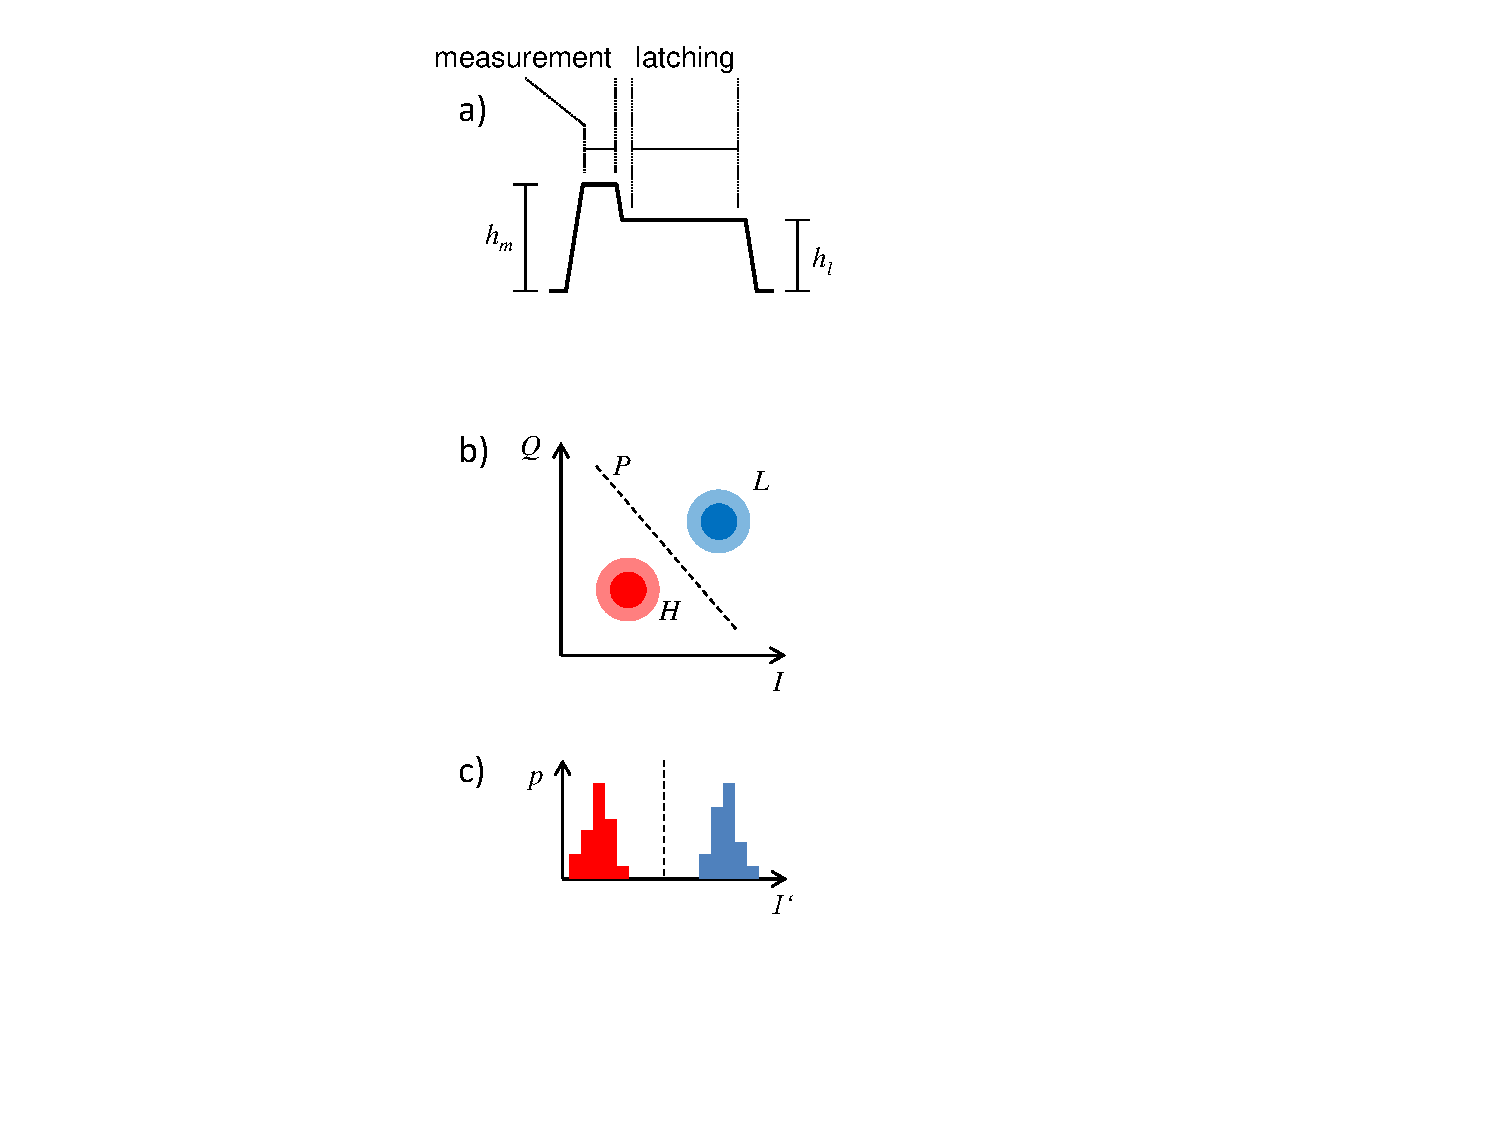
\includegraphics[width=\textwidth]{./material/figures/measurement/readout}
\caption{a) Microwave pulse envelope used for exciting the CJBA during readout. The pulse consists of a measurement part with amplitude $h_m$ and a latching part with ampliude $h_l<h_m$. To determine the state of the resonator during the latching interval, the phase of the reflected signal is meaused in the time window $t_m$. b) Distribution of the measured average $(I,Q)$ values in the IQ plane. The line $P$ that intersects the average quadratures $(I_0,Q_0)$ provides optimal separation between the two clusters corresponding to the state L and H of the resonator. c) Switching probability histograms corresponding to the distribution of the measured $(I,Q)$ values projected along the axis $\perp P$.}
\label{fig:readout_bringup}
\end{figure}

The general readout principle of the CJBA readout that we use in this work is described in section \ref{section:cjba}. Here we explain how we choose the frequency and drive amplitude working point for the readout. To bring up the readout, we first determine the resonance frequency $f_r$ of the CJBA by reflectometry, with the qubit in state $\ket{0}$ and largely detuned from the resonator. We then choose a relative drive detuning $\Omega>\sqrt{3}$ at which the bistable regime is accessible. Next, we mix a continous drive signal with a drive pulse as shown in fig. \ref{fig:readout_bringup}a. We then attenuate the resulting drive signal using a tunable attenuator at room temperature and send it to the CJBA. The reflected and amplified signal is then demodulated with the continous input drive signal using an IQ demodulator. The resulting I/Q quadrature signals are again amplified and get digitized by an ADC card at a sampling rate of 1 GHz during the time window $t_m$, as indicated in fig. \ref{fig:readout_bringup}a. We then average the digitized I/Q signals over the whole measurement window to obtain a single measurement point in the IQ plane and repeat this sequence a large number of times (typically $10^4$). We then repeat this whole procedure for various values of the input attenuation, each time calculating the estimated variance $\hat{\sigma}_{IQ}^2=\sum\limits_i ((I_i-\bar{I}_i)^2+\sum\limits_i (Q_i-\bar{Q}_i)^2)/n$ of the obtained data sets. When starting with a high attenuation and reducing it, at some point the input power sent to the CJBA will be sufficient to make it switch from the L to the H state, thereby changing the phase and consequently the average position of the I/Q values of the obtained signal. Since the switching is a stochasic process, we will observe two families of points close to the transition power. At an input power where approximately 50 \% of switching occurs, the variance $\sigma_{IQ}^2$ of the obtained IQ data points will be largest, as shown in fig. \ref{fig:readout_bringup}b. At this point, we can substract the averages $(I_0=\sum\limits_i I_i / n,Q_0 = \sum\limits_i Q_i/n)$ from the data and perform a principal axis transformation, which diagonalizes the covariance matrix
%
\begin{equation}
\mathrm{var}_{IQ} = \left(\begin{array}{cc}\mathrm{var}(I) & \mathrm{cov}(I,Q) \\ \mathrm{cov}(I,Q) & \mathrm{var}(Q) \end{array}\right)
\end{equation}
%
of the data. Using this transformation, we can project the measured (I,Q) data points on the axis $\perp P$, as shown in fig. \ref{fig:readout_bringup}, and obtain a one-dimensional switching probability distribution. The obtained offsets $I_0$, $Q_0$ and principal axis rotation angle $\alpha_{IQ}$ gives us then the discrimination criterion $Q_L<Q_0+\tan{\alpha_{IQ}}(I-I_0)$ that we can use to classify new data points as belonging to the L or H state at the chosen working point. Normally, if the measurement window $t_m$ is large enough and no retrapping occurs during the meausurement, the distributions corresponding to the L and H states will not overlap, yielding perfect discrimination between them.

\begin{SCfigure}[1][ht!]
\centering
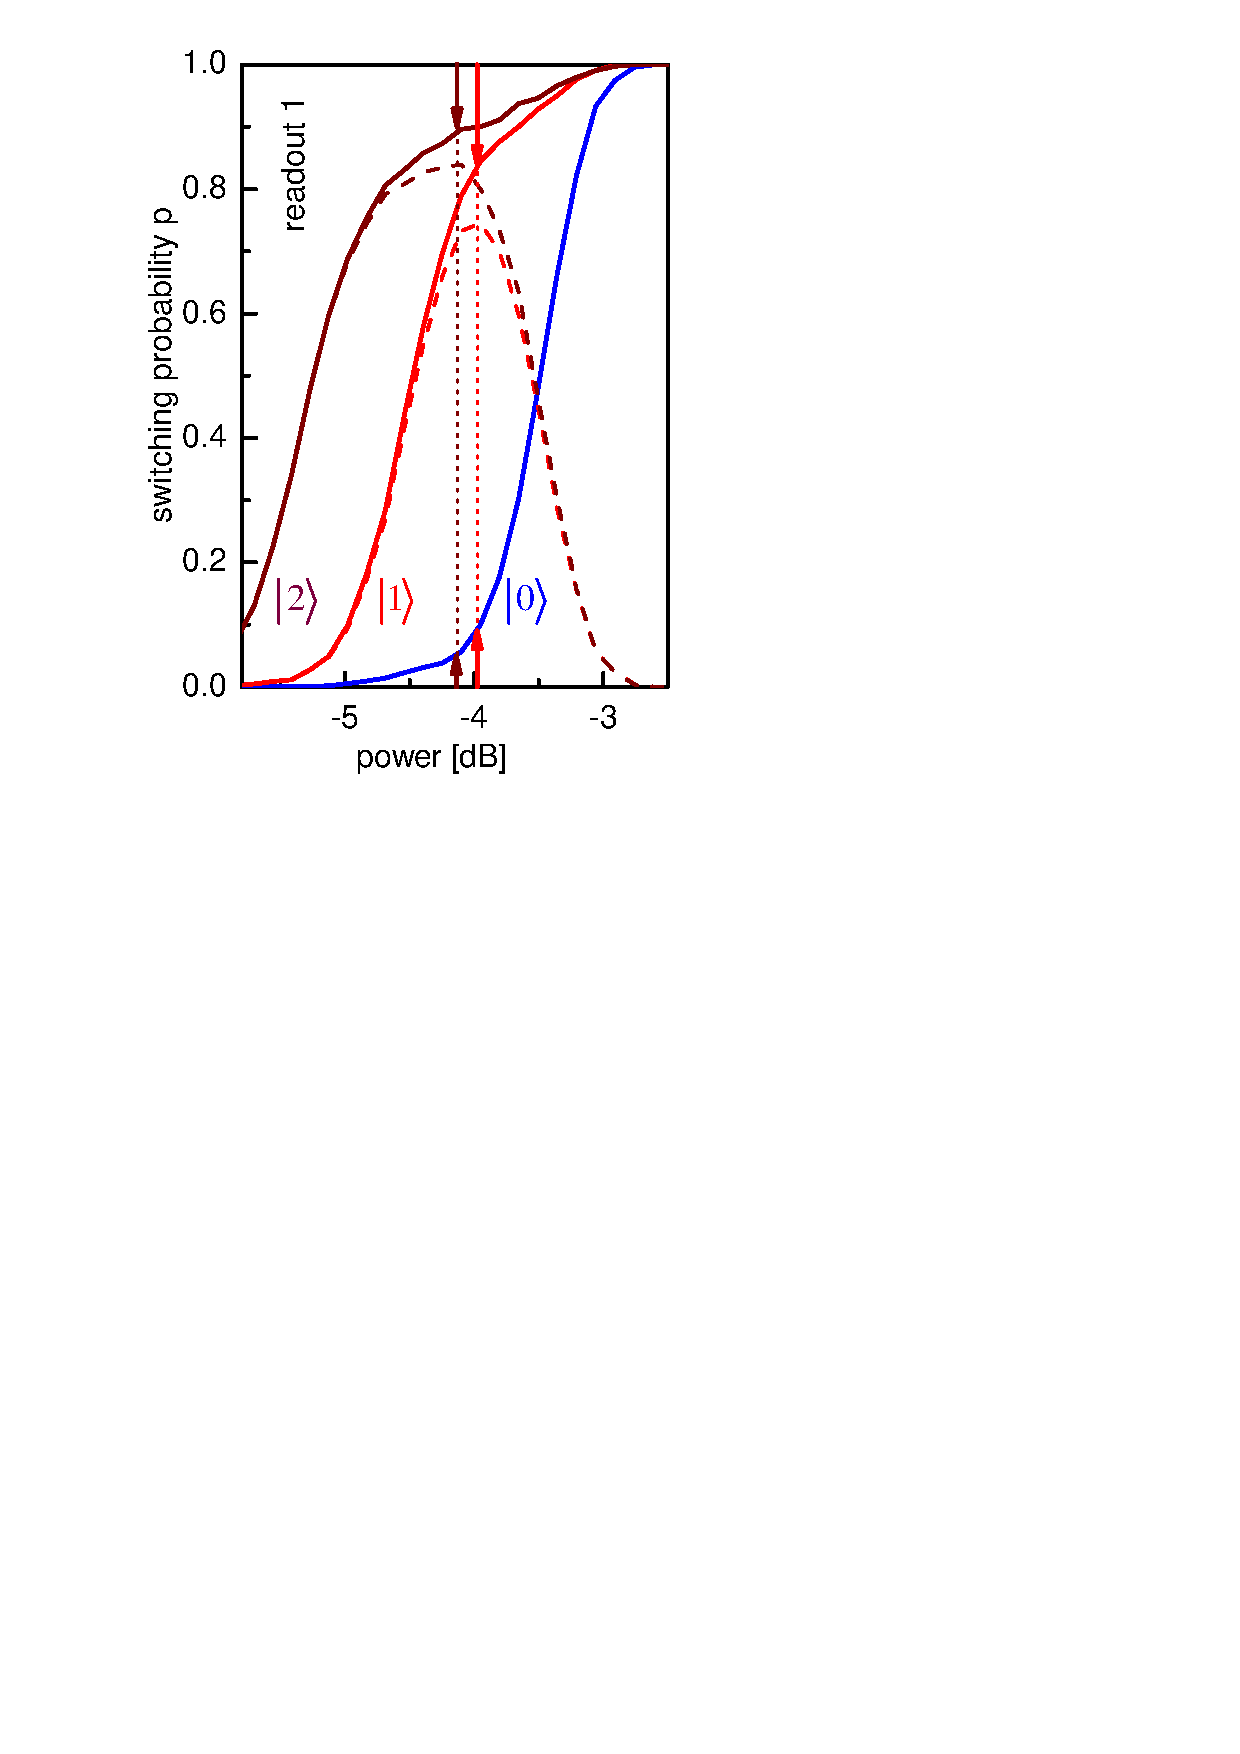
\includegraphics[width=0.4\textwidth]{./material/papers/grover/figures/s_curves_example}
\caption{Exemplary s-curve measurement for one of the qubits on the chip. Shown is the switching probability $p$ of the CJBA as a function of the readout signal power, plotted for different qubit states $\ket{0}$,$\ket{1}$ and $\ket{2}$. The readout contrast between different states is given as the probability difference between the associated switching probability curves. Light and dark red arrows indicate the optimal working points for the $c_{01}$ and $c_{02}$ readout contrasts, respectively.}
\label{fig:s_curves_example}
\end{SCfigure}

\smallskip

After having determined the $I_0$, $Q_0$ and $\alpha_{IQ}$, we slightly tune the attenuation such that we obtain $\approx 20\%$  of switching. At this working point, the readout contrast of the CJBA is usually already sufficient to perform a simple qubit spectroscopy, as described in section \ref{section:qubit_spectroscopy} and calibrate a $X_\pi$ Rabi pulse, as described in section \ref{section:qubit_rabi}. After having done this, we can measure the switching probability of the CJBA readout as a function of the input power while either leaving the qubit in state $\ket{0}$ or exciting it to the state $\ket{1}$. Fig. \ref{fig:s_curves_example} shows an example of such a measurement. Here, the difference $c_{01}$ between the two curves corresponding to the $\ket{1}$ and $\ket{0}$ states corresponds to the input-power dependent readout contrast and allows us to choose the optimum input power for the qubit readout. If desired, we can also perform a $X_\pi^{10}\cdot X_\pi^{12}$ pulse sequence on the qubit to bring it into the state $\ket{2}$ before the readout. In this state, the dispersive shift of the resonator frequency is larger than in the state $\ket{1}$, therefore resulting in a maximum readout contrast $\mathrm{max}(c_{02})>\mathrm{max}(c_{01})$, as shown in fig. \ref{fig:s_curves_example}, which is advantageous when performing e.g. single-run quantum algorithms on the processor, as described in chapter \ref{chapter:grover_algorithm}.

\section{Qubit Manipulation}

To drive the qubits, we need to generate fast microwave pulses with a well defined frequency and phase. As described in one of the previous paragraphs we can use IQ sideband mixing to shape arbitrary drive pulses of the form
%
\begin{equation}
u(t) = I(t)\cos{\omega_{LO}t}+Q(t)\sin{\omega_{LO}t}
\end{equation}
%
We can rewrite this as a product of two complex quantities
%
\begin{equation}
u(t) = \Re\left[ A(t)\cdot\exp{\left(-i\omega_{LO} t\right)}\right].
\end{equation}
%
The X axis of each qubits Bloch sphere is defined by the reference phase of the microwave pulse and can be chosen arbitrarily but must be conserved during one single experimental run. In addition, when performing experiments on multiple qubits, the phase differences between the reference phases of individual qubit drive signals must be conserved between individual runs of the experiment. Thus, to realize a rotation of the qubit state in the XY-plane of the Bloch sphere around an axis $\cos{\phi}\vec{X}+\sin{\phi}\vec{Y}$, we can use a Gaussian-shaped pulse of the form
%
\begin{equation}
A(t) = A_0\cdot\exp{\left(-\frac{(t-t_0)^2}{2\sigma_t}\right)}\cdot\exp{\left(-i\phi\right)}
\end{equation}
%
Here, we typically use a pulse rise time $\sigma_t=3\;\mathrm{ns}$. The advantage of using Gaussian pulses is that the Fourier transform of the pulse is again a Gaussian and, in contrast to a rectangular pulse, does not exhibit side lobes in the frequency domain \citep{bauer_gaussian_1984}. Whenever possible, we just change the height of this pulse to tune the Rabi angle of a given drive pulse. However, for large Rabi angles this is not possible, hence in that case we simply add a flat plateau to the top of the Gaussian pulse. In the following sections we explain how we use such microwave drive pulses to perform qubit spectroscopy, Rabi oscillations and decoherence time measurements.

\subsection{Spectroscopic Measurements of the Qubit State} \label{section:qubit_spectroscopy}

\begin{figure}[ht!]
\centering
a)\includegraphics[width=0.6\textwidth]{"./material/figures/measurement/qubit_spectroscopy"}
b)\includegraphics[width=0.6\textwidth]{"./data/ct5/2011_04_21 - grover and tomo/example - qubit 2 spectroscopy"}
\caption[]{a) Qubit drive and readout pulse sequence used for performing qubit spectroscopy. b) Example of a measured qubit spectroscopy. Shown is the switching probability of the qubit readout when driving the qubit with a very long drive pulse (typically 1 $\mu$s) at a given drive frequency. The resonance to the right (red data points) corresponds to the $\ket{0}\to\ket{1}$ transition of the qubit at frequency $f_{01}$, the resonance on the left (blue data points) to the 2-photon $\ket{0}\to\ket{2}$ transition at frequency $f_{02}/2$. We fit of the two resonances with a Lorentzian to obtain an estimate of the transition frequencies.}
\label{fig:qubit_spectroscopy_example}
\end{figure}

In order to characterize the transition frequency and anharmonicity of the qubit we perform spectroscopic measurements of the qubit state. For this we drive the qubit with a very long Rabi pulse (usually $> 500\;\mathrm{ns}$) at a frequency $\omega_d$. When the drive frequency $\omega_{d}$ is close to the $\omega_{01}$ frequency of the qubit, the drive pulse will induce a Rabi oscillation of the quantum state of the qubit. The induced rotation amplitude will be largest at $\omega_d=\omega_{01}$, Due to decoherence of the qubit during the driven evolution, the maximum probability for measuring the qubit in the state $\ket{1}$ after the pulse is limited to 50 \%. Furthermore, if the drive frequency is sufficiently far detuned from the qubit transition frequency such that $|\omega_d-\omega_{01}|\gg \Gamma^\phi$, no oscillation will be induced and hence the qubit will remain in the state $\ket{0}$. By repeating the pulse sequence shown in fig. \ref{fig:qubit_spectroscopy_example}a for a range of drive frequencies $\omega_d$, a full spectroscopy of the qubit can be obtained. Fig. \ref{fig:qubit_spectroscopy_example}b shows an example of this, where we show the probability of measuring the qubit in state $\ket{1}$ after applying a $1\;\mathrm{\mu s}$ Rabi pulse, plotted as a function of $\omega_d$ and shown for two different drive amplitudes. Here, the blue curve has been measured at $10\;\mathrm{dB}$ higher power than the red curve and shows the two-photon $\ket{0}\to\ket{2}$ transition of the qubit, which can be excited at sufficiently high drive power. By fitting the two resonance curves with a Lorentzian model we obtain the qubit frequencies $f_{01}$ and $f_{02}/2$ and thus the charging and Josephson energies of the qubit at the given working point.

\subsection{Rabi Oscillations} \label{section:qubit_rabi}

\begin{figure}[ht!]
\centering
a)\includegraphics[width=0.6\textwidth]{"./material/figures/measurement/qubit_rabi_oscillation"}
b)\includegraphics[width=0.6\textwidth]{"./data/ct5/2011_04_21 - grover and tomo/example - qubit 2 rabi"}
\caption[]{Example of a measured qubit Rabi experiment. Shown is the switching probability of the qubit readout when driving the qubit at $f_{01}$ with a Gaussian drive pulse of varying duration. The measurement results are not corrected for readout errors.}
\label{fig:qubit_rabi_example}
\end{figure}

After having obtained the proper qubit transition frequency $f_{01}$ using the technique described above, we can perform a Rabi oscillation experiment by driving the qubit for a well-defined time with a drive pulse at the $f_{01}$ transition frequency and measuring the state of the qubit directly afterwards. Figure \ref{fig:qubit_rabi_example}a shows the pulse sequence that we use for a Rabi experiment and fig. \ref{fig:qubit_rabi_example}b shows the resulting measurement data, plotting the readout switching probability as a function of the Rabi drive time. The blue points correspond to measured data whereas the continuous red line corresponds to a fit of a model of the form $p(t)=p_0+a\cos{(\Omega t)}\exp{(-\Gamma_1 t)}$ to the experimental data. As can be seen, the amplitude of the Rabi oscillations gets damped the longer the drive pulse becomes, which is due to relaxation and dephasing during the driven evolution of the qubit. Also, the maximum readout contrast is limited due to readout errors, as we explain in more detail in the following chapter. From the fit of the Rabi data we obtain the Rabi frequency $\Omega$, which we can then use to perform precise single-qubit rotations, as will be explained later. Due to the finite anharmonicity of the qubit, there will always be a leakage to the second excited state $\ket{2}$ of the qubit which gets the more relevant, the faster we drive the system. This leakage mechanism can be an important source of errors and very relevant to the experiments that we discuss later.

\section{Dephasing Time Measurement}

\begin{figure}[ht!]
\centering
a)\includegraphics[width=0.6\textwidth]{"./material/figures/measurement/qubit_ramsey_oscillation"}
b)\includegraphics[width=0.6\textwidth]{"./data/ct5/2011_04_21 - grover and tomo/example - qubit 2 ramsey"}
\caption[]{Example of a measured qubit Ramsey experiment. Shown is the switching probability of the qubit readout after performing a $X_{\pi/2}$-wait-$X_{\pi/2}$ drive sequence at a frequency $f_{01}-\delta f$. Fitting the resulting curve with an attenuated sine-wave model allows us to determine the $f_{01}$ frequency of the Qubit with high accuracy.}
\label{fig:qubit_ramsey_example}
\end{figure}

After having obtained the transition frequency $f_{01}$ of the qubit and the Rabi frequency $\Omega$, we can characterize the dephasing of the qubit by performing a so-called {\it Ramsey fringe experiment}. In this kind of experiment, we first perform a $Y_{\pi/2}$ rotation of the qubit from the state $\ket{0}$, obtaining thus a superposed qubit state of the form $1/\sqrt{2}(\ket{0}+\ket{1})$. Then we displace the qubit frequency by an amount $\Delta f$ by using e.g. a fast magnetic flux pulse and then let the qubit state evolve freely during a certain amount of time $\Delta t$. Finally, we apply another $Y_{\pi/2}$ pulse to the qubit and measure the state of the qubit directly afterwards. The experimental pulse sequence of this experiment is shown in fig. \ref{fig:qubit_ramsey_example}a. Since the qubit frequency relative to the drive reference frame has been deplaced during the free evolution, the qubit will acquire a phase $\Delta \phi = 2\pi\Delta f \Delta t$. The final state of the qubit after applying the second $Y_{\pi/2}$ pulse will therefore become
%
\begin{equation}
\ket{\phi_f} = \left(\begin{array}{cc} 1 & -1 \\ 1 & 1 \end{array} \right)\cdot\left(\begin{array}{c} 1 \\ e^{i\Delta\phi} \end{array}\right) = \left( \begin{array}{c} i\sin{\Delta\phi/2} \\ -\cos{\Delta\phi/2}\end{array}\right)
\end{equation}
%
Hence, the resulting state $\ket{\phi_f}$ will oscillate between the state $\ket{0}$ and $\ket{1}$ as a function of the delay with a frequency $\Delta f/2$. As before, due to dephasing and relaxation during the free evolution of the qubit state, the amplitude of these oscillations will decay. If the system dephasing time is limited by qubit relaxation, the decay will follow a Gaussian of the form $\exp{(-\Gamma t^2)}$, otherwise it will also exhibit an exponential decay $\simeq \exp{(-\Gamma t)}$. In the Ramsey sequence, instead of detuning the qubit frequency during the free evolution phase we can also simply detune the qubit drive frequency instead, thereby changing the drive reference frame instead of the real qubit frequency. If this detuning is small in comparision to the Rabi frequency $\Omega$, we will still be able to accurately perform the first $Y_{\pi/2}$ pulse. However, since the drive reference frequency is now slighty detuned from that of the qubit, the state in the drive reference frame will acquire a relative phase $\Delta f \Delta t$ during the free evolution phase. By fitting the experimental data obtained for such an experiment to a model of the form $p(\ket{1}) = p_0 +a\cos{(\Delta f \Delta t+\phi_0)}\exp{(-\Gamma_2 t^2/2)}$ we can obtain an estimate of $\Delta f$ and $\Gamma_2$, thereby characterizing the effective dephasing time of the qubit. Fig. \ref{fig:qubit_ramsey_example}b shows an example of measured Ramsey data with a corresponding fit. Furthermore, since we know the frequency detuning of the drive during the free evolution of the qubit we can substract it from the fitted value $\Delta f$ and obtain the residual detuning of the qubit frequency from the drive frequeny. This allows us to precisely determine the qubit frequency and to correct drive frequency errors with an accuracy of typically $100\;\mathrm{kHz}$. 

\section{Relaxation Time Measurement}

\begin{figure}[ht!]
\centering
a)\includegraphics[width=0.6\textwidth]{"./material/figures/measurement/qubit_t1_measurement"}
b)\includegraphics[width=0.6\textwidth]{"./data/ct5/2011_04_21 - grover and tomo/example - qubit 2 t1"}
\caption[]{Example of a qubit relaxation time measurement. Shown is the probability of measuring the qubit in state $\ket{1}$ as a function of the delay time between the preparation of the state $\ket{1}$ and the actual measurement of the qubit state. The decay of this probability follows an exponential law of the form $p(\ket{1})\simeq\exp{(-\Gamma_1 t)}$}
\label{fig:qubit_t1_example}
\end{figure}

We can characterize the relaxation time of the qubit by performing a simple experiment where we put the qubit in state $\ket{1}$ by applying a $X_{\pi}$ pulse and let it evolve freely afterwards for a given time before reading out its state, as shown in fig. \ref{fig:qubit_t1_example}a. Due to coupling of the qubit to its environment, relaxation to the ground state can occur during the free evolution. Hence, the longer we wait, the higher the probability that the qubit has relaxed to the ground state. An example of the resulting probability curve obtained through such an experiment is shown in fig. \ref{fig:qubit_t1_example}b. It shows the probability of measuring the qubit in state $\ket{1}$, plotted as a function of the delay between the initial state preparation and the measurement of its state. As can be seen, the probability decreases exponentially as a function of time. As before, in the curve the blue markers correspond to experimental data and the red line corresponds to a fit of this data to a model of the form $p(\ket{1}) = p_0+p_a\exp{(-\Gamma_1 t)}$. From this fit, we can then extract the relaxation rate $\Gamma_1$ of the qubit at the given working point. In the following chapter we will look more in detail at the relaxation time of both qubits of our processor as a function of their transition frequency and their detuning from the readout resonator.

\chapter{Characterizing the Two-Qubit Processor} \label{chapter:processor_characterization}

After having detailed the design of the processor and the measurement techniques employed in this work, we will discuss how we can characterize it to demonstrate the basic functionality that we need to run meaningful quantum algorithms. In particular we show how we can implement a robust two-qubit quantum gate that we will use in the following chapter to run a real-world quantum algorithm on our processor.

\smallskip

We begin the chapter by discussing the measurement of the basic qubit and readout parameters. We will then give a detailed overview of the relevant decoherence times and readout fidelities of our processor at different working points and discuss our strategy for optimizing these parameters during its operation. Afterward we will explain the realization of single-qubit gates together with possible error sources that we need to take into account. We also discuss in detail the generation and characterization of entanglement. Finally, we discuss the implementation of a universal two-qubit gate and its characterization through quantum process tomography.

\section{Qubit \& Readout Characterization}

\begin{figure}[ht!]
	\centering
		\includegraphics[width=1.\textwidth]{"./data/ct5/qubit frequencies/qubit_spectroscopy"}
	\label{fig:ProcessorSpectroscopy}
	\caption[Spectroscopy of the Two-Qubit Processor]{Spectroscopy of our two-qubit processor. Shown are the $\ket{0}\to\ket{1}$ ($\omega_{01}$) and $(\ket{0}\to\ket{2})/2$ ($\omega_{02}/2$) transition frequencies of the two qubits, together with a fitted analytical model of the qubit parameters. We also show the frequencies of the two readout resonators.}
\end{figure}

The first step in the characterization of the processor consists in obtaining all the relevant qubit and readout parameters. For this, we perform a set of measurements from which we obtain the qubit frequencies, anharmonicities, junction asymmetries, the inter-qubit coupling, the coupling to the microwave drive lines, the coupling of each qubit to its readout and the relaxation and dephasing times of the qubits. Most of these parameters, such as the drive and readout couplings as well as the relaxation and dephasing times are measured for a range of qubit frequencies, which will allow us later to pick an ideal working point for our two-qubit experiments. A detailed account of the measurement techniques employed here can be found in chapter \ref{chapter:measurement}. 

\subsubsection{Qubit Frequency, Anharmonicity and Asymmetry}

To obtain the Josephson and charging energies as well as the junction asymmetries of the qubits we perform spectroscopic measurements of the single-photon $\ket{0}\to \ket{1}$ and the two-photon $\ket{0}\to\ket{2}$ qubit transitions at different values of the external magnetic flux $\Phi_{ext}$. By fitting the resulting values $\omega_{01}(\Phi_{ext})$ and $\omega_{02}(\Phi_{ext})$ to a theoretical model we obtain all relevant qubit parameters. For our processor, these are $E_J^I / h = 36.2\; \mathrm{GHz}$, $E_c^I / h = 0.98 \; \mathrm{GHz}$ and $E_J^{II} / h = 43.1\; \mathrm{GHz}$, $E_C^{II} / h = 0.87 \; \mathrm{GHz}$ for the Josephson and charging energies of the two qubits, yielding anharmonicities $\alpha^I\approx 245\;\mathrm{MHz}$ and $\alpha^{II}\approx 220\;\mathrm{MHz}$. For the qubit junction asymmetries, we obtain $d^I = 0.2$, $d^{II} =  0.35$.

\subsubsection{Readout Parameters}

To obtain the resonance frequencies and quality factors of the readout resonators we perform a simple reflectometric measurement of the $S_{11}$ transmission coefficient of the resonators. The resulting frequencies are $\nu_R^I = 6.84 \; \mathrm{GHz}$ and $\nu_R^{II} = 6.70 \; \mathrm{GHz}$ with quality factors $Q^I \simeq Q^{II} = 730$. We measure the Kerr nonlinearity $K$ of the resonators by following the procedure given in \citep[p. 166]{palacios-laloy_superconducting_2010} and obtain $K^I / \nu_R^I \simeq K^{II} / \nu_R^{II} = -2.3\pm 0.5 \times 10^{-5}$.

\subsubsection{Qubit/Readout Coupling}

The coupling of the qubits to the readout resonators can be determined by spectroscopically measuring the avoided level crossing between the two systems. For this, we perform a series of spectroscopic measurements of the resonator while tuning the qubit frequency from a value below the resonator frequency to one above it. The results of these measurements are given in fig. \ref{fig:qubit_resonator_anticrossing} and clearly show an avoided level crossing between the two systems. By fitting the obtained data to a theoretical model, we obtain the qubit-resonator coupling coefficients $g_{01}^I \simeq g_{01}^{II} = 2\pi\cdot 50 \; \mathrm{MHz}$.

\begin{figure}[htb!]
	\centering
	\includegraphics[width=1\textwidth]{"./data/ct5/cavity anticrossing/qubits_anticrossing_bw"}
	\caption[Spectroscopic measurement of the avoided level crossing between the two qubits and their corresponding readout resonator]{Spectroscopic measurement of the avoided level crossing between the two qubits and their corresponding readout resonator, yielding an effective qubit-resonator coupling strength $2g_{01}/2\pi\approx 50\;\mathrm{MHz}$.}
	\label{fig:qubit_resonator_anticrossing}
\end{figure}


\subsubsection{Qubit Parameter Survey}

\begin{figure}[ht!]
   \centering
	 \includegraphics[width=1\textwidth]{"./data/ct5/qubits - parameter surveys/qubit parameters"}
	 \caption[A qubit parameter survey showing $T_1$, readout contrast and Rabi frequency of the two qubits over a range of qubit frequencies]{A qubit parameter survey showing the relaxation time $T_1$, the readout contrast and the Rabi frequency at a fixed drive amplitude for the two qubits over a large range of qubit frequencies.}
	 \label{fig:qubit_parameters}
\end{figure}

In order to determine the optimal working point for our processor we need to characterize the properties of the qubits at many different frequencies. For this, we perform an automated survey where we measure the transition frequencies $\omega_{01}$ and $\omega_{02}$, the readout contrast $c$ and the relaxation and dephasing times $T_1$ and $T_2$ of each qubit at different values of the magnetic flux $\Phi_{ext}$. The results of such a parameter survey are summarized in fig \ref{fig:qubit_parameters}, where we show the relaxation time $T_1$,  the readout contrast $c_{01}$ and the Rabi frequency $f_{Rabi}$ at fixed drive amplitude for the two qubits within a frequency range between 5.2 and 6.5 GHz. As can be seen, the relaxation time of the qubits tends to increase the farther detuned each qubit is from its readout resonator. Not surprisingly, the drive frequency of the qubit also decreases when the qubit-resonator detuning increases, as expected from the Purcell effect, which filters incoming microwave signals that are far-detuned from the resonator frequency. The readout contrast decreases nearly linear when increasing the qubit-resonator detuning $\Delta$, as expected from the dispersive shift $\chi\propto 1/\Delta$ given by eq. (\ref{eq:stark_shift}).

\smallskip

It is interesting to note the non-monotonous characteristic of the qubit relaxation time $T_1$ shown in fig. \ref{fig:qubit_parameters}, which cannot be explained by Purcell-filtering through the readout resonator and hints thus at a different qubit relaxation process present in the system. A possible explanation would be the coupling of the qubit to spurious low-Q resonances in the environment. For example, the coupling of the qubit to volumetric resonance modes of the sample holder or to non-CPW resonance modes of the readout resonator could be possible explanations for the data. Also, the overall dependency of the relaxation time $T_1$ on the qubit-resonator detuning --ignoring the ``fine-structure'' present in the system-- is not quadratic as would be expected from the Purcell theory but rather linear. Also, by comparing the qubit relaxation time to the Rabi drive frequency reveals that the increase in $T_1$ is clearly not proportional to the Purcell factor, that determines both the qubit relaxation rate through the readout resonator and the Rabi drive frequency. However, the observed $T_1$ dependency can be partially explained by taking into account the qubit relaxation through the fast fluxline, which might be too strongly coupled to the qubit, hence inducing additional qubit relaxation beyond the Purcell and intrinsic qubit relaxation rates.

\section{Choice of Processor Working Points}

Having characterized all parameters of the qubits as a function of their frequencies $\omega_{01}^I$ and $\omega_{01}^{II}$, we go ahead and choose frequency working points for qubit manipulation and readout. For single-qubit manipulation and parking, we choose the two operating frequencies $\omega_{01,m}^I/2\pi = 5.247\;\mathrm{GHz}$ and $\omega_{01,m}^{II}/2\pi = 5.125\;\mathrm{GHz}$, where we have relaxation times $T_1^I(\omega_{01,m}^I) \approx 440\;\mathrm{ns}$ and $T_1^{II}(\omega_{01,m}^{II})\approx 520\;\mathrm{ns}$. For qubit readout, we choose $\omega_{01,r}^I \approx 6.2\;\mathrm{GHz}$ and $\omega_{01,r}^{II}\approx 6.0\;\mathrm{GHz}$, where we have single-shot readout contrasts $c_{01}^I(\omega_{01,r}^I)\approx 75\%$ and $c_{01}^{II}(\omega_{01,r}^{II})\approx 73\%$.

\section{Qubit Readout Characterization} \label{section:readout_matrix}

The readout errors of the qubits are fully characterized by the conditional switching probabilities $p_m(0|0)$ and $p_m(1|1)$, where we define $p_m(x|y)$ as the probability of obtaining a readout value $x$ after having prepared a qubit state $\ket{y}$, where $x,y\in\{0,1\}$ for single-qubit readout and $x,y\in\{00,01,10,11\}$ for two-qubit readout. In addition, a two-qubit readout usually exhibits readout crosstalk errors, which are characterized by the switching probabilities $p_m(x*|x0)=p_m(x0|x0)+p_m(x1|x0)$, $p_m(x*|x1)=p_m(x0|x1)+p_m(x1|x1)$ as well as $p_m(*x|0x)=p_m(0x|0x)+p_m(1x|0x)$ and $p_m(*x|1x)=p_m(0x|1x)+p_m(1x|1x)$, where $x\in\{0,1\}$. If crosstalk is present, $p_m(x*|x0) \ne p_m(x*|x1)$ and/or $p_m(*x|0x) \ne p_m(*x|1x)$.

\smallskip

\begin{SCfigure}[1.0][ht!]
	\centering
	\includegraphics[width=0.5\textwidth]{"./data/ct5/2011_04_21 - grover and tomo/good_data/readout_matrix_no_shelving"}
	\caption{The measured readout matrix of our two-qubit processor. Shown are the conditional measurement probabilities $p_m(x|y)$ where $x,y\in\{00,01,10,11\}$. The diagonal elements correspond to the readout fidelities of the four basis states. The single qubit readout fidelities as obtained from the matrix are $p_m^I(0*|00)=0.88$, $p_m^I(1*|10)=0.85$, $p_m^{II}(*0|00)=0.9$ and $p_m^{II}(*1|01)=0.85$, the readout crosstalks are $p_m(0*|00) - p_m(0*|01)=-0.01$, $p_m(1*|10) - p_m(1*|11)=-0.02$, $p_m(*0|00) - p_m(*0|10)=0$ and $p_m(*1|01) - p_m(*1|11)=-0.01$.}
	\label{fig:readout_matrix_no_shelving}
\end{SCfigure}

The single-qubit fidelities $p_m(0|0)$ and $p_m(1|1)$ can be simply obtained from an s-curve measurement, as explained in section \ref{section:qubit_readout}. In order to obtain the two-qubit readout errors, we perform an experiment where we measure the full set of conditional probabilities $p(x|y)$ with $x,y\in\{00,01,10,11\}$ by initializing the qubit register to each basis state and performing a simultaneous readout of the two qubits. By repeating and averaging the resulting readout outcomes $i$ for each basis state $\ket{j}$, where $\{i,j\}\in\{00,01,10,11\}$, we obtain the full set of conditional readout probabilities, which can be plotted as a $4\times 4$ readout matrix $\mathbf{R}$, as shown in fig. \ref{fig:readout_matrix_no_shelving}. From this matrix, all conditional and unconditional readout fidelities as well as the readout crosstalk can be calculated. We can correct a measured set of probabilities $\mathbf{p}_R=(p_{00},p_{01},p_{10},p_{11})$ for readout errors by simply multiplying it with the inverse of $\mathbf{R}$, such that $\mathbf{p}_R^{corr}=\mathbf{p}_R\cdot \mathbf{R}^{-1}$. For all experiments discussed in the remainder of this chapter, we will always correct readout errors by this method, unless indicated otherwise.

\section{Single-Qubit Operations}

\begin{figure}[ht!]
	\centering
		\includegraphics[width=1.\textwidth]{"./data/ct5/2010_12_01 - iq tomography/iq_tomographies"}
	\caption[Demonstration of single-qubit XY control]{Demonstration of single-qubit XY control. The figures show the state probability of a single qubit when preparing it in one of the states $\ket{1}$, $1/\sqrt{2}(\ket{0}+\ket{1})$ or $1/\sqrt{2}(\ket{0}+i\ket{1})$ and subjecting it to a microwave drive pulse of constant duration with $a(t) = V_I\cdot\cos{\omega_{rf}t}+V_Q\cdot\sin{\omega_{rf}t}$ and of varying amplitudes $V_I$ and $V_Q$.}
	\label{fig:single_qubit_iq_control}
\end{figure}

To perform arbitrary single-qubit operations -- as needed e.g. for implementing a quantum algorithm or performing quantum state tomography -- we need to implement a universal set of $X$, $Y$ and $Z$ qubit gates on our processor. Qubit rotations in the $XY$-plane are implemented through microwave drive pulses, where the phase of the drive pulse in reference to an arbitrary reference determines the rotation axis and the amplitude of the drive pulse the Rabi frequency of the gate. To characterize the drive pulses, we perform an experiment where we initialize a single-qubit in the states $\ket{1}$, $1/\sqrt{2}(\ket{0}+\ket{1})$ and $\sqrt{2}(\ket{0}+i\ket{1})$ and subject it afterward to a single microwave pulse of the form $a(t) = V_I\cdot\cos{\omega_{rf}t}+V_Q\cdot\sin{\omega_{rf}t}$, which we tune by changing the input voltages $V_I$ and $V_Q$ to the $IQ$-mixer that generates the pulse from a continuous input microwave-tone at frequency $\omega_{rf}$. We then measure the qubit state $\ket{1}$ occupation probability at different values of $V_I$, $V_Q$, obtaining the graph shown in fig. \ref{fig:single_qubit_iq_control}. The qubit which was prepared in state $\ket{1}$ shows a perfectly cylinder-symmetric switching probability pattern when subjecting it to an IQ-pulse of a given phase, which is indeed what one would expect for a qubit being prepared in either the $\ket{0}$ or $\ket{1}$ state. On the other hand, the switching probability distributions of the qubits prepared in the states $1/\sqrt{2}(\ket{0}+\ket{1})$ and $1/\sqrt{2}(\ket{0}+i\ket{1})$ are mirror-symmetric, where the switching probability does not vary at all along the drive axis that corresponds to the axis along which the qubit has been prepared. These measurements demonstrate our ability to prepare and drive the qubit along arbitrary axes of the Bloch sphere, which is a necessary prerequisite for implementing a universal set of gates on our processor and for performing quantum state tomography.

\section{Two Qubit Operations}

\begin{figure}[ht!]
	\centering
		\includegraphics[width=0.7\textwidth]{"./data/ct5/2011_04_11 - anticrossing/qubit_anticrossing_modified"}
	\caption[Spectroscopic measurement of the avoided level crossing between the two qubits of our processor]{a) Spectroscopy measurement of the avoided level crossing between the two qubits of our processor. b) Single spectroscopy of qubit I when in resonance with qubit II. From this spectroscopic measurement, a qubit-qubit coupling strength of $2g_{qq}=8.3\;\mathrm{MHz}$ can be deduced. }
	\label{fig:qubit_anticrossing}
\end{figure}

We use the capacitive coupling between the qubits to implement two-qubit gates and to create entangled states between them. To characterize the qubit-qubit interaction, we first perform a spectroscopic measurement of the qubits. For this, we measure a spectroscopy of qubit I for a range of external fluxes $\Phi_{ext}^I$, such that the frequency of qubit I $\omega_{01}^I$ gets tuned through the frequency of qubit II $\omega_{01}^{II}$. Now, if the two qubit frequencies $\omega_{01}^I$, $\omega_{01}^{II}$ are far detuned such that $|\omega_{01}^I-\omega_{01}^{II}|\gg 2g_{qq}$, the eigenstates of the coupled two-qubit Hamiltonian correspond to a very good accuracy to the independent qubit states $\ket{01}$ and $\ket{10}$. Therefore, far from the resonance condition we observe only one spectroscopic line corresponding to the transition $\ket{00}\to\ket{10}$ (since we drive only the first qubit). However, close to resonance, the eigenstates of the two-qubit system approach the two Bell states $\ket{\Psi_\pm} = 1/\sqrt{2}(\ket{10}\pm\ket{01})$, which can both be excited by driving qubit I. Hence we observe two spectroscopic lines corresponding to the two transitions $\ket{00}\to 1/\sqrt{2}(\ket{01}+\ket{10})$ and $\ket{00}\to 1/\sqrt{2}(\ket{01}-\ket{10})$. The frequency width of the gap between these two spectroscopic lines corresponds to the qubit-qubit coupling strength $2g_{qq}/2\pi$. Fig \ref{fig:qubit_anticrossing} shows the results of such a spectroscopic measurement, where qubit II was positioned at a $\omega_{01}^I/2\pi = 5.125\;\mathrm{GHz}$ and the frequency of qubit II was tuned from $\omega_{01}^{II}/2\pi\in 5.1-5.15\;\mathrm{GHz}$. At resonance, we measure a coupling strength of $2g_{qq}/2\pi = 8.3\;\mathrm{MHz}$.

\subsection{Creation of Entanglement} \label{section:creation_of_entanglement}

\begin{SCfigure}[1][ht!]
	\centering
	\includegraphics[width=0.6\textwidth]{"./material/figures/measurement/qubit_swap"}
	\caption[Pulse sequence used to create an entangled two-qubit state]{Pulse sequence used to create an entangled two-qubit state using a non-adiabatic pulse that brings the qubits in resonance for a well-defined time.}
	\label{fig:qubit_swap_pulse_sequence}
\end{SCfigure}

After having characterized the qubit-qubit interaction using a spectroscopic measurement we perform a coherent swapping operation between the qubits. We implement this operation by non-adiabatically changing the resonance frequency of the qubits from an off-resonance condition $|\omega_{01}^I-\omega_{01}^{II}|\gg g_{qq}$ to an on-resonance condition $\omega_{01}^I=\omega_{01}^{II}$. When doing this after preparing the qubits in one of the states $\ket{01}$ or $\ket{10}$, we induce a coherent energy swap between them. We then terminate the interaction after a well-defined time and measure the state of the two-qubit register directly afterward. When the qubits are in resonance, the time evolution operator of their quantum state is given as
%
\begin{equation}
U(t)=\left(\begin{array}{cccc}
1 & 0 & 0 & 0\\
0 & \cos{(tg_{qq})} & i\sin{(tg_{qq})} & 0\\
0 & i\sin{(tg_{qq})} & \cos{(tg_{qq})} & 0\\
0 & 0 & 0 & 1\end{array}\right)_{\left\{ \left|00\right\rangle ,\left|01\right\rangle ,\left|10\right\rangle ,\left|11\right\rangle \right\} } \label{eq:swap_evolution_operator_main}
\end{equation}
%
As can be seen, the two basis states $\ket{01}$ and $\ket{10}$ indeed oscillate back and forth between each other with frequency $g_{qq}$. The states $\ket{00}$ and $\ket{11}$ are not affected by the interaction.

\smallskip

\begin{figure}[ht!]
	\centering
	\includegraphics[width=0.7\textwidth]{"./material/papers/iswap/figures/swap_raw_and_corrected"}
	\caption[]{State occupation probabilities for the two-qubit register during a coherent energy swap. a) Shows the raw state probabilities corresponding to the states $\ket{00}$, $\ket{01}$, $\ket{10}$ and $\ket{11}$, b) shows the same data corrected for the limited visibility of each qubit readout and c) shows the fully corrected readout data where we account for both visibility and inter-qubit readout crosstalk errors.}
	\label{fig:swap_raw_and_corrected}
\end{figure}

Fig. \ref{fig:qubit_swap_pulse_sequence} summarizes the frequency, drive and measurement pulse sequence that we use for this experiment. When varying the time during which the qubits are in resonance, we can observe the coherent swapping of energy between them. Figure \ref{fig:swap_raw_and_corrected} presents the results of such a measurement. Shown are the measured qubit state probabilities $p(\ket{00})$, $p(\ket{01})$, $p(\ket{10})$ and $p(\ket{11})$ as a function of the swap duration $\Delta t$. Subfigure a) shows the raw, uncorrected readout data, subfigure b) shows the probabilities corrected for limited readout visibility and subfigure c) shown the probabilities corrected for both limited readout visibility and crosstalk, using the readout matrix discussed in section \ref{section:readout_matrix}. The oscillatory behavior between the states $\ket{01}$ and $\ket{10}$ is clearly visible in the data. Also, the frequency of the energy swap $2g_{qq}=8.3\;\mathrm{MHz}$ agrees with the value obtained from the spectroscopic measurement. Fig. \ref{fig:swap_raw_and_corrected}c shows, in addition to the measured state occupation probabilities a master equation simulation of the experiment, that the Hamiltonian and Lindblad operators discussed in section \ref{section:master_equation}. This simulation takes into account relaxation and dephasing of the qubits. The relaxation rates used in the simulation correspond to the experimentally measured relaxation rates at the operating frequencies of the qubits, whereas the dephasing rates were free fitting parameters. We do not use the measured single-qubit dephasing rates in our simulation since they do not correspond to the effective dephasing rate of the two-qubit system at resonance, which cannot be described within the master equation formalism. The reason for this is that the transition frequency of the two eigenstates $\ket{\phi_\pm}=1/\sqrt{2}(\ket{01}\pm\ket{10})$ at resonance $\omega_{01}^{\pm}=\omega_{01}^{I,II}\pm\sqrt{4g_{qq}^2+\Delta^2}/2\approx \omega_{01}^{I,II}\pm g_{qq} +\Delta^2/8g_{qq}$ is insensitive to variations of $\Delta$ to first order. Hence, the effective dephasing rate of the two-qubit system will be much higher than the single-qubit dephasing rates. To reproduce the experimentally observed dephasing, we therefore used effective dephasing rates $\Gamma_\phi^{I,II}=2\;\mathrm{\mu s}$. As can be seen, using these rates and the measured relaxation rates as well as coupling parameter $g_{qq}$, the simulation agrees well with the experimental data.


\subsection{Quantum State Tomography}

The experiments that we describe in the following sections often require us to determine the density matrix of an experimental two-qubit state. The method that we use for this purpose is called {\it quantum state tomography} (QST) (see e.g. \cite{nielsen_quantum_2000} for an overview of this method). In this section, we therefore explain in detail the procedure that we use to perform QST. Furthermore, we also discuss several sources of errors occurring in standard QST and how we can estimate their effect on our results.

\smallskip

The density matrix of an n-qubit system can be written as
%
\begin{eqnarray}
\rho & = & \sum\limits_{v_1,v_2\hdots v_n} \frac{c_{v_1,v_2\hdots v_n} \hat{\sigma}_{v_1}\otimes \hat{\sigma}_{v_2}\hdots \hat{\sigma}_{v_n}}{2^n} \label{eq:state_tomography_state_representation} \\
c_{v_1,v_2\hdots v_n} & = & \mathrm{Tr}\left\{\hat{\sigma}_{v_1}\otimes \hat{\sigma}_{v_2}\hdots \otimes\hat{\sigma}_{v_n} \; \rho \right\} \label{eq:state_tomography_coefficients}
\end{eqnarray}
%
where $v_i \in \left\{ X,Y,Z,I\right\}$ and $n$ gives the number of qubits in the system and where the $c_{v_1,v_2\hdots v_n}$ are real-valued coefficients that describe the given density matrix. To reconstruct the density matrix of an experimental quantum system, it is thus sufficient to measure the expectation values of these $n^2-1$ coefficients on an ensemble of identically prepared states. For our two qubit system, this means measuring all possible combinations of the operators $\{I,\hat{\sigma}_x^I,\hat{\sigma}_y^I,\hat{\sigma}_z^I\}\otimes\{I,\hat{\sigma}_x^{II},\hat{\sigma}_y^{II},\hat{\sigma}_z^{II}\}$. However, in our experiments, we can only measure the $\hat{\sigma}_z$ operator of the qubit, therefore, rather than measuring the $\hat{\sigma}_x$ and $\hat{\sigma}_z$ operators directly, we rotate the quantum state of each qubit such that the state vector along the desired measurement axis coincides with the z-axis of the Bloch sphere and then measure $\hat{\sigma}_z$ instead.

When using this direct method, statistical and systematic measurement errors can produce a set of coefficients $v_i$ that corresponds to a {\it non-physical} density matrix, i.e. a density matrix which violates either the positivity $\bra{\psi}\rho\ket{\psi} > 0$ (for all valid states $\ket{\psi}$) or the unity-trace condition $\mathrm{Tr}(\rho)=1$. To alleviate this problem, several techniques can be employed. In the following section we discuss an estimation technique which is able to overcome the problem of non-physical density matrices, the so-called {\it maximum likelihood estimation}.

\subsubsection{Maximum Likelihood Estimation of Quantum States}

Maximum likelihood estimation is a method that numerically or analytically maximizes a likelihood function that is based on a number of measured outcomes and and a set of parameters that need to be estimated. The set of parameters that corresponds to the maximum of the probability function can then be interpreted as the one with the highest probability of generating the observed outcomes. When estimating the parameters of a density matrix with this method, the probability function to be maximized is the joint probability of obtaining the measured values $\{c_{X,X,\hdots,X},c_{Y,X,\hdots,X},\hdots,c_{I,I,\hdots,I}\}$ for a given density matrix $\hat{\rho}$. By numerically or analytically maximizing this joint probability over the set of possible density matrices we obtain the density matrix which is most likely to have produced the set of measurement outcomes that we have observed.

The joint measurement operators $\hat{\Sigma}_j = \hat{\sigma}_{v_1}\otimes \hat{\sigma}_{v_2}\hdots \otimes\hat{\sigma}_{v_n}$ have the eigenvalues $\pm 1$ and can thus be written as 
\begin{equation}
\hat{\sigma}_{v_1}\otimes \hat{\sigma}_{v_2}\hdots \otimes\hat{\sigma}_{v_n} = \ket{+_j}\bra{+_j}-\ket{-_j}\bra{-_j} \label{eq:ml_operators}
\end{equation}
where $\ket{-_j}$ and $\ket{-_j}$ are the eigenstates corresponding to the eigenvalues $\pm 1$ of $\hat{\Sigma}_j$. When performing $l$ measurements of the operator $\hat{\Sigma}_j$, the expectation value $\langle \hat{\Sigma}_j \rangle$ can be estimated as
%
\begin{equation}
\widehat{\langle \hat{\Sigma}_j \rangle}_\rho = \frac{1}{l}\sum\limits_{i = 1}^l m_i(\hat{\Sigma}_j,\rho) \label{eq:tomography_measurement_estimator}
\end{equation}
where $m_i(\hat{\Sigma},\rho)$ denotes the outcome of the $i$-th measurement of the operator $\hat{\Sigma}$ on the state described by the density matrix $\rho$. Since each outcome $m_i(\hat{\Sigma}_j,\rho)$ is Bernoulli distributed, the sum $\widehat{\langle\hat{\Sigma_j}\rangle}_\rho$ of them is binomially distributed with an expectation value \mbox{$E(\widehat{\langle \hat{\Sigma}_j \rangle}_\rho) = \langle \hat{\Sigma}_j \rangle_\rho$} and the variance $\sigma^2(\widehat{\langle \hat{\Sigma}_j \rangle}_\rho) = 1/l \cdot (1-\langle \hat{\Sigma}_j \rangle_\rho^2)$. For large sample sizes $l$, the binomial distribution can be well approximated by a normal distribution with the same expectation value and variance. The joint probability of obtaining a set of estimates $\{s_1,\hdots,s_{n^2-1}\}$ for the set of operators $\{\langle\hat{\Sigma}_1 \rangle_\rho,\hdots,\langle\hat{\Sigma}_{n^2-1} \rangle_\rho\}$ for a proposed density matrix $\rho$ is thus given as
%
\begin{equation}
P\left(\widehat{\langle \hat{\Sigma}_1 \rangle }_\rho = s_1;\hdots;\widehat{\langle \hat{\Sigma}_{n^2-1} \rangle}_\rho =  s_{n^2-1}\right) = \prod\limits_{i = 1}^{n^2-1} \exp{\left(-\frac{l}{2}\frac{(s_i-\langle \hat{\Sigma}_i \rangle_\rho)^2}{1-\langle \hat{\Sigma}_i \rangle_\rho^2}\right)}
\end{equation}
%
By maximizing this probability (or the logarithm of it) as a function of the parameters of the proposed density matrix $\rho$, we obtain the $\rho$ which has the highest probability of having produced the observed measurement values. 

\subsubsection{Including Experimental Tomography Errors}

The ML technique also allows us to include further optimization parameters when calculating the joint probability. This is useful for modeling e.g. systematic errors of the measurement or preparation process, which can be described by modifying the operators contained in the probability sum. A common source of errors in our tomography measurements are shifts in the amplitude and phase of the microwave pulses used to drive the qubit. We are obliged to rotate the qubit state when performing state tomography since our measurement apparatus permits us only to measure the $\hat{\sigma}_z$ operator of each qubit. We can therefore replace the operators $\hat{\sigma}_x$ and $\hat{\sigma}_y$ in eq. (\ref{eq:ml_operators}) with an effective measurement of $\hat{\sigma}_z$ preceded by a rotation $R_{X,Y}$ given as
\begin{eqnarray}
R_{X} & = & \exp{\left( -i \hat{\sigma}_y \pi / 4\right)} \\
R_{Y} & = & \exp{\left( +i \hat{\sigma}_x \pi / 4\right)} 
\end{eqnarray}
Within this model, phase and amplitude errors can be modeled by including additional phase factors, yielding
\begin{eqnarray}
R_{X}' & = & \exp{\left( -i \left[+\hat{\sigma}_y\cos{\alpha}+\hat{\sigma}_x\sin{\alpha} \right] \left[\pi / 4+\gamma\right]\right)} \\
R_{Y}' & = & \exp{\left( +i \left[-\hat{\sigma}_y\sin{\beta}+\hat{\sigma}_x\cos{\beta}\right] \left[\pi / 4+\delta\right]\right)} 
\end{eqnarray}
Here, $\alpha$ and $\beta$ represent phase errors whereas $\gamma$ and $\delta$ represent amplitude errors in the drive pulses. A detailed discussion of how we fit these parameters to experimental data will be given in section \ref{section:tomographic_errors}.

\subsection{Characterizing Two-Qubit States using QST}

\begin{figure}[ht!]
	\centering
	\begin{tabular}{ll}
	a) & b) \\
	\includegraphics[width=0.48\textwidth]{"./data/ct5/2011_04_21 - grover and tomo/good_data/pauli_set_2"} & \includegraphics[width=0.48\textwidth]{"./data/ct5/2011_04_21 - grover and tomo/good_data/pauli_set_3"} \\
	c) & d) \\
	\includegraphics[width=0.48\textwidth]{"./data/ct5/2011_04_21 - grover and tomo/good_data/input_matrices_1"} & \includegraphics[width=0.48\textwidth]{"./data/ct5/2011_04_21 - grover and tomo/good_data/output_matrices_1"} \\
	\end{tabular}
	\caption[]{a/b) Measured Pauli sets of a prepared $\ket{01}$ input state and a corresponding output state (b) measured after a swapping time $t=31\;\mathrm{ns}$, showing the measured values of the single-qubit and multi-qubit Pauli operators. c/d) Corresponding density matrices of the input and output states, reconstructed using maximum likelihood estimation. The absolute value $|\rho_{ij}|$ of each element of the density matrix is represented by the size of each circle, whereas the phase $\angle \rho_{ij}$ is represented both by the color of the circle and the direction of the arrow. The state fidelities compared to the ideal states $\ket{\psi^{in}}=\ket{01}$ and $\ket{\psi^{out}}=1/\sqrt{2}(\ket{01}+i\ket{10})$ are $F^{in}_{tr}=94\%$ and $F^{out}_{tr}=84\%$, respectively. The density matrices of the ideal states are overlaid in black, for comparison.}
	\label{fig:pauli_set_example}
\end{figure}

Using quantum state tomography, we can repeat the swapping experiment described in section \ref{section:creation_of_entanglement} and reconstruct the full experimental density matrix of our system at many different times during the swap sequence by measuring a full Pauli set on an ensemble of identically prepared state. Fig. \ref{fig:pauli_set_example} shows an example of two experimentally measured Pauli sets and their associated density matrices, measured at swapping times $t=0\;\mathrm{ns}$ and $t= 31\;\mathrm{ns}$. As can be seen, the obtained density matrix a) corresponds closely to a pure quantum state $\ket{01}$ with a fidelity $F_{tr}=94\%$, whereas the density matrix d) corresponds to an entangled two-qubit state $1/\sqrt{2}(\ket{01}+\ket{10})$with fidelity $F_{tr}=84\%$. 

\smallskip

Measuring Pauli sets at different times, we can follow the evolution of the quantum state during the course of the swap. Fig. \ref{fig:swap_pauli_set_vs_time_with_simulation} shows the result of such an experiment, where we plot the measured values of all Pauli operators as a function of the swapping time between the qubits. The red and green curves correspond to the single-qubit Pauli operators $\hat{\sigma}^I_{X,Y,Z}\otimes \mathrm{I}$ and $\mathrm{I}\otimes \hat{\sigma}^{II}_{X,Y,Z}$, the blue curves to the two-qubit Pauli operators $\hat{\sigma}_{X,Y,Z}^I\otimes \hat{\sigma}_{X,Y,Z}^{II}$. The dashed line corresponds to a master equation simulation of the swapping experiment, where the qubit coupling, relaxation and dephasing parameters are chosen in accordance with experimental values. As can be seen, the simulation agrees well with the experimental data. Deviation between data and simulation can be seen in the $\hat{\sigma}_{X,Y}^I\otimes \hat{\sigma}_{X,Y}^{II}$ operators and is caused by an additional phase acquired by the qubits during the swap, which appears due to the fact that we have to shift the frequency of the qubits to bring them in resonance, hence we acquire a dynamical phase in the frame rotating at the uncoupled qubit frequencies. In addition, experimental drift of our measurement equipment may induce an additional phase factor during the measurement, which takes several hours to complete.

\smallskip

In the margins of this thesis book, we show the full set of density matrices at all moments during the swap, as obtained from the measured Pauli sets shown in fig. \ref{fig:swap_pauli_set_vs_time_with_simulation}. When following the evolution of the quantum state as a function of time (by flipping the pages of the book) the coherent energy swap between the two qubits can be observed, the coherence of the two-qubit state decreasing steadily during the swap due to qubit dephasing and relaxation.

\begin{figure}[ht!]
   \centering
	 \includegraphics[width=1.\textwidth]{"./data/ct5/film of swap/pauli_set_vs_time_with_simulation"}
	 \caption[]{Measured Pauli operators $\hat{\sigma}_i \otimes \hat{\sigma}_j$ with $i,j \in \{X,Y,Z,I\}$ as a function of the interaction time. Shown are the 6 single-qubit operators as well as the 9 two-qubit correlation operators. The dashed line represents a master-equation simulation of the experiment.}
	 \label{fig:swap_pauli_set_vs_time_with_simulation}
\end{figure}

\subsection{Creation of Bell states}

We can use the ML method presented above to perform state tomography of entangled Bell states that we create by using the swapping interaction between the qubits. In general, the four Bell states are
%
\begin{eqnarray}
\ket{\Psi_+} = \frac{1}{\sqrt{2}}\left(\ket{01}+\ket{10}\right) \\
\ket{\Psi_-} = \frac{1}{\sqrt{2}}\left(\ket{01}-\ket{10}\right) \\
\ket{\Phi_+} = \frac{1}{\sqrt{2}}\left(\ket{00}+\ket{11}\right) \\
\ket{\Phi_-} = \frac{1}{\sqrt{2}}\left(\ket{00}-\ket{11}\right)
\end{eqnarray}
%

\begin{SCfigure}[1.0][htb!]
	\centering
	\includegraphics[width=9cm]{"./material/figures/measurement/bell_state_creation"}
	\caption[]{Pulse sequence used to experimentally generate entangled Bell states. The sequence consists in exciting one of the qubits to the state $\ket{1}$, creating an entangled state using the swapping interaction and correcting the acquired phase of the state. For the $\ket{\Phi_\pm}$ states, we use an additional $Y(\pi)$ pulse at the end of the sequence.}
	\label{fig:bell_generation_pulse_sequence}
\end{SCfigure}


The experimental protocol that we use for generating a Bell state is shown in fig. \ref{fig:bell_generation_pulse_sequence}. In essence, we use the swapping interaction between the qubits to create an entangled state and adjust the acquired dynamic phase of that state by a short z-pulse. To create the $\Phi_+$ and $\Phi_-$ states we use a $X(\pi)$ pulse at the end of the sequence in addition. Finally we perform quantum state tomography on the created state to reconstruct its density matrix. In fig. \ref{fig:bell_states} we show the reconstructed density matrices of the four created Bell states. The trace fidelity $\bra{\psi}\rho\ket{\psi}$ between the experimentally created and ideal state is shown on top of the density matrix and ranges between $83 \%$ and $87 \%$.

\begin{figure}[ht!]
  \flushright
	\includegraphics[width=1\textwidth]{"./data/ct5/2011_02_09 preparation of bell states/bell matrices"}
	\caption{Reconstructed density matrices of experimentally created Bell states. Shown are the states $\ket{\Psi_\pm}=1/\sqrt{2}(\ket{01}\pm\ket{10})$ and $\ket{\Phi_\pm}=1/\sqrt{2}(\ket{00}\pm\ket{11})$. The trace fidelities of the density matrices, $F_{tr}=\bra{\psi}\rho\ket{\psi}$ range between 83 \% and 87 \%.}
	\label{fig:bell_states}
\end{figure}

\subsection{Violation of the Bell Inequality}

After having showed that we can create superposition states of the two qubits using the swapping interaction, we proceed to demonstrate that we have actually created entangled qubit states by performing a so called {\it Bell test} on our two-qubit system. In this section, we will give an introduction to this test and explain how we implement it on our two-qubit processor.

\smallskip

In a famous 1935 paper \citep{einstein_can_1935}, A. Einstein, B. Podolsky and N. Rosen (EPR) point out that quantum mechanics can be considered ``incomplete'' if one assumes that a set of simple physical principles holds true. These two principles are {\it locality} and {\it realism}, together often referred to as {\it local realism}. The principle of locality states that an object is influenced directly only by its immediate surroundings, or stated differently, that no interaction between any two objects may propagate faster than the speed of light. The principle of realism states that any physical observable has, at all times, a pre-existing measurement value which exists independent of any actual measurement of the observable. In their paper, Einstein, Podolsky and Rosen showed that within standard quantum mechanics it is possible to write down quantum states that, when performing certain measurements on them, clearly violate at least one of the principles of locality or realism. As an example, take the state
%
\begin{equation}
\ket{\psi} = \frac{1}{\sqrt{2}}\left(\ket{\uparrow \downarrow}+\ket{\downarrow \uparrow}\right) \label{eq:epr_example}
\end{equation}
%
which describes a system of two spin 1/2 particles that is in a superposition between the $\ket{\uparrow \downarrow}$ and $\ket{\downarrow \uparrow}$ states. Now, when separating the two particles by a large distance and measuring the value of one of the spins --such that by the assumption of locality, no information exchange can take place between the two systems--, the wave function of the system will collapse in either of the two states $\ket{\uparrow \downarrow}$ or $\ket{\downarrow \uparrow}$. Hence, a measurement of one of the particles will instantaneously change the spin state of the other particle, seemingly violating the principle of locality by which no instantaneous information exchange can take place between two distant systems. In their paper, Einstein, Podolsky and Rosen called this effect {\it spooky action at a distance}.

\smallskip

However, the violation of locality can be resolved by assuming that the state of the quantum system does  possess a well-defined value before actually measuring it. This would imply that our description of the quantum-mechanical state as given by eq. (\ref{eq:epr_example}) is just missing some additional, {\it hidden variables} that contain the information on the spin of each particle and which are not accessible by us. A hypothetical theory that contains these hidden variables and could thus complete the quantum mechanical description of the particle is usually referred to as a {\it hidden variable theory}.

\smallskip

In 1964, J. Bell provided a mathematical description of locality and realism and devised an experimental test of the hypothesis formulated by Einstein {\it et. al.} \citep{bell_einstein_1964}. Building on his work, J. Clauser, M. Horne, A. Shimony and R. Holt proposed an actual experiment to test the hypotheses of quantum mechanics against hidden-variable or non-local theories as formulated in the Bell and EPR papers \cite{clauser_proposed_1969}. The first successful realization of this proposed experiment was achieved by A. Aspect {\it et. al.} \cite{aspect_experimental_1982} and confirmed the validity of quantum mechanics, showing that either the assumption of realism or that of locality must be false. In the following decades, several more experiments have been performed to test the Bell hypothesis, trying to close several so-called {\it loopholes}. Such a loophole is a problem of the experimental setup or design that affects the validity of the experimental findings. Typical loopholes affecting Bell-type experiments are the {\it detection efficiency} or {\it fair sampling}, the {\it communication} or {\it locality} and the {\it rotational invariance} loophole. We will discuss the loopholes most relevant to our own experiment in the following paragraph.

\smallskip

To test the Bell inequality with our two-qubit setup, we follow the experimental procedure proposed by Clauser {\it et. al.} \citep{clauser_proposed_1969}. According to their proposal, we first prepare an entangled two-qubit state of the form
%
\begin{equation}
\ket{\phi} = \frac{1}{\sqrt{2}}\left(\ket{01}+e^{-i\varphi}\ket{10}\right) \label{eq:chsh_state}
\end{equation}
%
On this quantum state we measure then the expectation value of the operator
%
\begin{equation}
\mathrm{CHSH} = \mathrm{QS}+\mathrm{RS}+\mathrm{RT}-\mathrm{QT}
\end{equation}
%
where the individual operators $\mathrm{Q,R,S,T}$ are given as
%
\begin{eqnarray}
	\begin{array}{cccccccc}
		\mathrm{Q} & = & \hat{\sigma}_z^1 &&& \mathrm{S} & = & \hat{\sigma}_z^2\cdot \cos{\phi}+\hat{\sigma}_x^2 \cdot \sin{\phi} \\
		\mathrm{R} & = & \hat{\sigma}_x^1 &&& \mathrm{T} & = & -\hat{\sigma}_z^2\cdot \sin{\phi}+\hat{\sigma}_x^2 \cdot \cos{\phi}
	\end{array}
\end{eqnarray} 
%
Here, the angle $\phi$ is a parameter that gives the rotation of the measurement basis in respect to the $z$ axis and should be chosen in accordance to the phase $\varphi$ of the entangled qubit state to which the operator is applied. To obtain the value of $\bracket{\mathrm{CHSH}}$, we measure $\bracket{\mathrm{QS}}$, $\bracket{\mathrm{RS}}$, $\bracket{\mathrm{RT}}$ and $\bracket{\mathrm{QT}}$ on an ensemble of identically prepared quantum states. For a classical state without entanglement, the operator $\bracket{\mathrm{CHSH}}$ is bound by
%
\begin{equation}
\left|\bracket{\mathrm{CHSH}}\right| \le 2. \label{eq:chsh_max}
\end{equation}
%
However, for an entangled quantum state, the maximum value of the operator is given as $2\sqrt{2}$. 

\smallskip

\begin{SCfigure}[1.0][ht!]
	\centering
	\includegraphics[width=9cm]{"./material/figures/measurement/chsh"}
	\caption[]{Experimental pulse sequence used in the CHSH experiment. It consists in exciting one of the qubits to the state $\ket{1}$, bringing it in resonance with the other qubit for a well-defined duration, performing single-qubit rotations to align the qubit state with the desired measurement basis and finally measuring the $\bracket{\hat{\sigma}_z^I\cdot\hat{\sigma}_z^{II}}$ operator of the two-qubit register.}
	\label{fig:chsh_pulse_sequence}
\end{SCfigure}

The pulse sequence used for generating an entangled two-qubit state and measuring the CHSH operator on it is shown in fig. \ref{fig:chsh_pulse_sequence}. As before, we generate the state by exciting one of the qubits to the state $\ket{1}$ and bringing it in resonance with the other qubit for a well-defined duration. Afterward, we apply single-qubit rotations to align the qubit state with the axis along which we want to perform the measurement. Finally we measure the $\bracket{\hat{\sigma}_z^I\cdot \hat{\sigma}_z^{II}}$ operator of the rotated qubit state. We then repeat this procedure on an ensemble of identically prepared input states for all of the four individual operators of CHSH operator. Figure \ref{fig:chsh} shows the results of such a measurement. As can be seen, the operator $\bracket{\mathrm{CHSH}}$ varies sinusoidally as a function of the rotation $\phi$ of the measurement basis. The maximum and minimum of the raw value of $\bracket{\mathrm{CHSH}}$ reaches $\approx 1.4$, thereby failing to violate the boundary for non-classical states as given by eq. (\ref{eq:chsh_max}). However, when accounting for the readout errors in our experiment, the corrected CHSH data reaches a maximum value $\approx 2.52$, thereby violating the classical boundary of the CHSH equation. We can hence violate the Bell inequality with our two-qubit processor, however we are not able to close the detector efficiency loophole. In addition, due to the measurement time required to determine the state of each qubit and the close proximity of the two qubits, we are not able to close the communication or locality loophole either. However, when accepting the general validity of quantum mechanics, the violation of the Bell inequality with the generated two-qubit states can still serve as an entanglement witness and confirm that we are able to generate entangled, non-classical quantum states with our processor.

\begin{figure}[ht!]
	\centering
		\includegraphics[width=0.8\textwidth]{./material/papers/iswap/figures/chsh}
	\caption[]{Value of the $\bracket{\mathrm{CHSH}}$ operator measured for an ensemble of identically prepared Bell states $1/\sqrt{2}(\ket{01}+e^{-i\varphi}\ket{10})$, plotted as a function of the rotation $\phi$ of the measurement basis. Blue markers correspond to raw measurement data, red markers to data corrected for readout errors. The solid line represents the best fit to the theory. The inset shows the standard deviation $\sigma$ of the maximum value of the $\bracket{\mathrm{CHSH}}$ operator as a function of the sample size. For large sample sizes, $\sigma$ is limited by experimental drift of the measurement basis.}
	\label{fig:chsh}
\end{figure}

\subsubsection{Errors} 

Besides obvious readout errors, the main source of errors in our experiment is drift of the measurement equipment. Most importantly, the phase of the arbitrary waveform generator (AWG), which generates the sideband pulses for driving the qubit, can drift in respect to the phases of the microwave sources, thereby changing the effective phase of the measurement basis of the CHSH operator. Fig. \ref{fig:chsh_drift} illustrates the effect of this drift on the phase of the generated Bell state. Shown is the phase of the state $\ket{\phi}$ as given by eq. (\ref{eq:chsh_state}) extracted from a full CHSH data set as shown in fig. \ref{fig:chsh}. When repeatedly measuring $\varphi$ over a long time period, oscillations with an amplitude of $\approx 40^\circ$ can be observed. This drift can be explained by a time shift of the AWG of the order of $200\;\mathrm{ps}$, which has indeed been observed independently using a fast oscilloscope.

\begin{SCfigure}[1.0][hb!]
	\centering
	\includegraphics[width=9cm]{"./data/ct5/2011_03_17 - chsh/chsh_drift"}
	\caption[]{Phase $\varphi$ of an experimentally generated Bell state as a function of time. The phase exhibits oscillatory drift of the order of $\approx 40^\circ$ being caused by a time offset drift of the AWG.}
	\label{fig:chsh_drift}
\end{SCfigure}

\section{Realizing a Two-Qubit Gate}

We have demonstrated that it is possible to create highly entangled qubit states with our processor by preparing Bell states, performing quantum state tomography and violating the Bell inequality. However, to realize a universal two-qubit quantum processor, it is necessary to implement a so-called {\it universal two-qubit gate}. Therefore, in the following sections we discuss how to realize and characterize such a gate.

\subsection{Principle}

By definition, a universal two-qubit gate together with a set of universal one-qubit gates, allows us to create any possible two-qubit quantum state \citep{barenco_elementary_1995}. In principle, there are (infinitely) many choices for possible universal two-qubit gates. In this work, we are interested mainly in the so-called $\sqrt{i\mathrm{SWAP}}$ gate, which has the representation
%
\begin{equation}
U(t)=\left(\begin{array}{cccc}
1 & 0 & 0 & 0\\
0 & 1/\sqrt{2} & i/\sqrt{2} & 0\\
0 & i/\sqrt{2} & 1/\sqrt{2} & 0\\
0 & 0 & 0 & 1\end{array}\right)_{\left\{ \left|00\right\rangle ,\left|01\right\rangle ,\left|10\right\rangle ,\left|11\right\rangle \right\} } \label{eq:sqrt_iswap_gate_main}
\end{equation}
%
We can implement this gate naturally using the swapping interaction as given by eq. (\ref{eq:swap_evolution_operator_main}) when letting the qubits evolve in resonance for a time $t_{\sqrt{i\mathrm{SWAP}}}=1/8g$, which, for our experimental value of $2g = 8.3\;\mathrm{MHz}$ corresponds to $t_{\sqrt{i\mathrm{SWAP}}}\approx 30\;\mathrm{ns}$. 

\subsection{Experimental Implementation}

Figure \ref{fig:iswap_pulse_sequence} shows the pulse sequence that we use to realize the $\sqrt{i\mathrm{SWAP}}$ gate with our processor for an exemplary input state. In the case shown, we excite the first qubit to the state $\ket{1}$, creating an input state $\ket{10}$. We then tune in resonance the two qubits for a time $t_{\sqrt{i\mathrm{SWAP}}}$. After tuning the qubits out of resonance again, we apply two single-qubit $Z$-gates to compensate the dynamical phases acquired during the swap. Then, we optionally apply single-qubit tomography gates and finally read out the qubit state at the optimal readout working point. Using this technique, we can reconstruct the density matrix of the quantum state after applying the two-qubit gate to it. Similarly, we can perform quantum state tomography on the input state to obtain its density matrix. Reconstructing the input and output density matrices for a range of different input state will then allow us to fully characterize the gate operation, as discussed in the next section.

\begin{figure}[ht!]
	\centering
		\includegraphics[width=0.8\textwidth]{./material/papers/iswap/figures/iswap_gate_pulse_sequence}
	\caption{Experimental pulse sequence used for implementing the two-qubit $\sqrt{i\mathrm{SWAP}}$ gate. The sequence shown for an exemplary input state $\ket{10}$ consists in exciting the first qubit to the state $\ket{1}$, bringing the qubits in resonance for a time $t=1/8g$, separating them and compensating the acquired dynamical phases by using two single-qubit $Z$-pulses. Finally, optional tomographic pulses are applied before reading out the qubit state at the optimal readout frequencies of the qubits.}
	\label{fig:iswap_pulse_sequence}
\end{figure}


\subsection{Quantum Process Tomography of the Gate}

To characterize the fidelity of our quantum gate, we perform so-called {\it quantum process tomography} \citep{poyatos_complete_1997}. This procedure allows us to fully characterize an experimental quantum process, such as our implementation of the $\sqrt{iSWAP}$ gate. The approach that we use in this work is called {\it standard quantum process tomography} (SQPT). There exist other common methods such as ancilla-assisted quantum process tomography \citep{dur_nonlocal_2001,dariano_quantum_2001,altepeter_ancilla-assisted_2003}, that we will not discuss since they are not relevant to this work.

\smallskip

In the following section we discuss the experimental implementation of standard quantum process tomography on our two-qubit processor.

\subsubsection{Theoretical Description of a Quantum Process}

A quantum process as described in section \ref{section:master_equation} can be described by a set of Kraus operators, as given by eq. (\ref{eq:kraus_representation}):
%
\begin{equation}
\LA{A}(\rho_A) = \sum\limits_i^{N_k} E_i \rho_A E_i^\dagger \label{eq:kraus_representation_2}
\end{equation}
%
If we express these operators $E_i$ in a different operator basis $\tilde{E}_j$ such that $E_i = \sum_j a_{ij} \tilde{E}_{j}$ and insert into eq. (\ref{eq:kraus_representation_2}), we obtain

\begin{eqnarray}
 \mathcal{E}(\rho) & = & \sum\limits_i \sum\limits_j a_{ij} \tilde{E}_j \;\rho\; \sum\limits_k a_{ik}^* \tilde{E}_k^\dagger \\
& = & \sum\limits_{j,k}\tilde{E}_j \; \rho \; \tilde{E}_k^\dagger \sum\limits_i a_{ij} a_{ik}^* \\
& = & \sum\limits_{j,k}\tilde{E}_j \; \rho \; \tilde{E}_k^\dagger \; \chi_{jk} \label{eq:process_chi_representation}
\end{eqnarray}
where we defined $\chi_{jk} = \sum\limits_i a_{ij} a_{ik}^*$. This is the so-called $\chi$-matrix representation of the quantum process. Here, all the information on the process is contained in the matrix $\chi$, which controls the action of the now process-independent operators $\tilde{E}_i$ on the initial density matrix $\rho$.

\subsubsection{Implementation}

As said before, the goal of QPT is to obtain the coefficients of the $\chi$-matrix -- or any other complete parametrization of the process -- from a set of experimentally measured density matrices $\{\rho_i\}$ and $\{\mathcal{E}(\rho_i)\}$. Standard process tomography \citep{nielsen_quantum_2000,poyatos_complete_1997} can be implemented for our two-qubit gate by using the following procedure:

\begin{enumerate}
\item Choose a set of operators $E_i$ that forms a full basis of $\mathcal{M}: Q_1 \to Q_2$. For n-qubit process tomography we usually choose $E_{i_1,i_2 \hdots i_n} = \hat{\sigma}_{i_1}\otimes \hat{\sigma}_{i_2}\hdots\otimes\hat{\sigma}_{i_n}$, where $\hat{\sigma}_i$ are the single-qubit Pauli operators and $i\in\{I,X,Y,Z\}$. For a Hilbert space of dimension $n$, this yields $4^n-1$ operators (excluding the trivial operator $I^{\otimes n}$).
\item Choose $4^n$ pure quantum states $\ket{\phi_i}$ such that the basis $\{\ket{\phi_1}\bra{\phi_1}$, $\ket{\phi_1}\bra{\phi_2}\hdots$, $\ket{\phi_{4^n}}\bra{\phi_{4^n-1}},\ket{\phi_{4^n}}\bra{\phi_{4^n}}\}$ spans the whole space of input density matrices $\rho$. Usually, for a n-qubit system we choose $\phi = \{\ket{0},\ket{1},(\ket{0}+\ket{1})/\sqrt{2},(\ket{0}+i\ket{1})/\sqrt{2}\}^{\otimes n}$, where $^{\otimes n}$ denotes the n-dimensional Kronecker product of all possible permutations.
\item For each of the $\ket{\phi_i}$, determine $\mathcal{E}(\ket{\phi_i}\bra{\phi_i})$ by quantum state tomography. Usually we also determine $\ket{\phi_i}\bra{\phi_i}$ experimentally since the preparation of this state already entails small preparation errors that should be taken into account when performing quantum process tomography. 
\end{enumerate}

After having obtained the $\rho_i$ and $\mathcal{E}(\rho_i)$ we get the $\chi$-matrix by the following procedure: First, we write $\mathcal{E}(\rho_i) = \sum_j \lambda_{ij} \tilde{\rho}_j$, with some arbitrary basis $\tilde{\rho}_j$ and
letting $\tilde{E}_m \tilde{\rho}_j \tilde{E}_n^\dagger = \sum_k \beta_{jk}^{mn}\tilde{\rho}_k$. We can then insert into eq. (\ref{eq:process_chi_representation}) and obtain
\begin{eqnarray}
\sum\limits_k \lambda_{ik} \tilde{\rho}_k & = & \sum\limits_{m,n} \chi_{mn} \sum\limits_k \beta_{ik}^{mn} \tilde{\rho}_k  
\end{eqnarray}
This directly yields $\lambda_{ik} = \sum_{m,n}\beta_{ik}^{mn}\; \chi_{mn}$, which, by linear inversion,  gives $\chi$. Hence, we can fully characterize a quantum process acting on an $n$-dimensional Hilbert space by measuring $2\cdot 4^n$ experimental density matrices (or $4^n$ when assuming that no errors occur during the preparation of the input states, which thereby are known).

\smallskip

Similar to quantum state tomography, experimental errors occurring during quantum process tomography can produce a process matrix $\chi$ that is {\it non-physical} in the sense that the resulting quantum process does not obey the three axioms stated in section \ref{section:master_equation}. Therefore, we render the obtained $\chi$ matrix physical by numerically searching the  physical process matrix $\chi_{ph}$ that has the smallest distance to the original one $d=\|\chi-\chi_{ph}\|$.

\subsubsection{From the $\chi$ matrix to the Kraus representation}

To go back from the $\chi$-matrix representation of the quantum process to the Kraus form, we write each process-independent operator $\tilde{E}_i$ as a sum of all the Kraus operators $E_l$, such that
%
\begin{equation}
	\tilde{E}_i = \sum\limits_l a_{il}\; E_l
\end{equation}
%
Inserting this into eq. (\ref{eq:process_chi_representation}) we obtain
%
\begin{eqnarray}
\begin{mathcal}E\end{mathcal}(\rho) & = & \sum\limits_{j,k}\chi_{jk}\sum\limits_{l,m} a_{jl}a_{km}^* E_l \rho E_m^\dagger   \label{eq:process_chi_transformed} \\
& = & \sum\limits_i E_i \rho E^\dagger_i
\end{eqnarray}
%
We find hence that $\sum\limits_{j,k} \chi_{jk}a_{jl}a_{km}^* = \delta_l^m$, or, written in matrix form $A\chi A^\dagger = \mathrm{I}$. This identity is true for $A$ being the matrix of eigenvectors of $\chi$, multiplied by the square root of the corresponding matrix of eigenvalues. It is thus easy to obtain the Kraus representation of the quantum process by diagonalizing the Hermitian matrix $\chi$.

\smallskip

The Kraus operator form of the quantum process is useful since it allows us to easily visualize the different operators acting on the density matrix $\rho$. By ordering the Kraus operators as a function of their associated eigenvalues we can easily visualize the different unitary and non-unitary processes acting together on the density matrix $\rho$.

\subsubsection{Experimental Results: Input/Output Matrices And $\chi$-Matrix}

\begin{figure}[p]
	\centering
		\includegraphics[width=1.0\textwidth]{"./data/ct5/2011_04_21 - grover and tomo/good_data/process -matrices 1"}
	\caption{The experimental input-output density matrices of the quantum process tomography of the $\sqrt{i\mathrm{SWAP}}$ gate. Shown are the measured density matrices of 16 different input states and the corresponding output matrices with their state fidelities. The ideal matrices are overlaid in black. (part I/II)}
	\label{fig:process_matrices_1}
\end{figure}

\begin{figure}[p]
	\centering
		\includegraphics[width=1\textwidth]{"./data/ct5/2011_04_21 - grover and tomo/good_data/process -matrices 2"}
	\caption{The experimental input-output density matrices of the quantum process tomography of the $\sqrt{i\mathrm{SWAP}}$ gate. Shown are the measured density matrices of 16 different input states and the corresponding output matrices with their state fidelities. The ideal matrices are overlaid in black. (part II/II)}
	\label{fig:process_matrices_1}
\end{figure}

We perform standard process tomography of our two-qubit gate by following the procedure outlined in the last sections. Figs. \ref{fig:process_matrices_1} and \ref{fig:process_matrices_1} summarize the experimentally determined input-output density matrices, measured for our two-qubit $\sqrt{i\mathrm{SWAP}}$ quantum gate. We show pairs of corresponding input and output states together, showing both the reconstructed experimental density matrices as well as the ideal ones. The input states are annotated below the corresponding density matrices. Above each matrix we show the trace fidelity between it and the ideal quantum state. A total of 16 input/output pairs has been measured, corresponding to a complete set of states necessary to characterize the quantum process of our gate operation.

\smallskip

\begin{figure}[ht!]
	\centering
		\includegraphics[width=1.\textwidth]{./material/papers/iswap/figures/chi_matrix_and_error_process}
	\caption{The reconstructed $\chi$ matrix of our implementation of the $\sqrt{i\mathrm{SWAP}}$ quantum gate. a) shows the lower half of the Hermitian matrix. b) shows the product $\tilde{\chi}=\chi\cdot\chi_{id}^{-1}$ of the measured $\chi$ matrix and the ideal process matrix $\chi_{id}$. The colored arrows connecting different elements of $\tilde{\chi}$ indicate unitary and non-unitary error processes to which the corresponding matrix elements can be associated.}
	\label{fig:chi_matrix_and_errors}
\end{figure}

From the input/output matrices, we can easily calculate the $\chi$ matrix of the quantum process by the method described above. The resulting matrix is shown in fig. \ref{fig:chi_matrix_and_errors}. There, we show the experimentally obtained $\chi$ matrix of our $\sqrt{i\mathrm{SWAP}}$ gate as well as the error process defined as $\tilde{\chi} = \chi\cdot\chi_{id}$, where $\chi_{id}$ corresponds to the ideal gate process. $\chi_{id}$ is as well shown as black outlines overlaid to the measured $\chi$ matrix. The arrows connecting different parts of the $\tilde{\chi}$ matrix group several unitary and non-unitary error processes that can be attributed to the individual elements.

\subsection{Gate Fidelity}

After having obtained the experimental $\chi$ matrix, it is trivial to calculate the process fidelity, which is defined as $F=\mathrm{Tr}\{\chi_{id}\cdot\chi\}$, where $\chi_{id}$ corresponds to the ideal quantum process. For our experimental process matrix, it is given as $F=0.9$. The fidelity can be roughly compared to the output state fidelity averaged over the whole set of possible input density matrices.

\subsection{Gate Error Analysis}

When analyzing experimental errors of our implementation of the $\sqrt{iSWAP}$ gate, we treat unitary and non-unitary gate errors as well as tomography errors. The former are associated to errors in the quantum process itself, whereas the latter are caused by unitary and non-unitary errors during quantum state tomography.

\smallskip

\subsubsection{Tomographic Errors} \label{section:tomographic_errors}

Tomographic errors are removed from the process map of our $\sqrt{iSWAP}$
gate using the following method: The measured Pauli sets corresponding
to the sixteen input states are first fitted by a model including
errors both in the preparation of the state (index $prep$) and in
the tomographic pulses (index $tomo$). The errors included are angular
errors $\varepsilon_{\mathrm{I,II}}^{\mathrm{prep}}$ on the nominal
$\pi$ rotations around $X_{\mathrm{I,II}}$, $\eta_{\mathrm{I,II}}^{\mathrm{prep,tomo}}$and
$\delta_{\mathrm{I,II}}^{\mathrm{prep,tomo}}$ on the nominal $\pi/2$
rotations around $X_{\mathrm{I,II}}$ and $Y_{\mathrm{I,II}}$, a
possible departure $\xi_{\mathrm{I,II}}$ from orthogonality of $\left(\overrightarrow{X_{\mathrm{I}}},\overrightarrow{Y_{\mathrm{I}}}\right)$
and $\left(\overrightarrow{X_{\mathrm{II}}},\overrightarrow{Y_{\mathrm{II}}}\right)$,
and a possible rotation $\mu_{\mathrm{I,II}}$ of the tomographic
$XY$ frame with respect to the preparation one. The rotation operators
used for preparing the states and doing their tomography are thus
given by

\[
\begin{array}{c}
X_{\mathrm{I,II}}^{\mathrm{prep}}(\pi)=e^{-\mathrm{i}\left(\pi+\varepsilon_{\mathrm{I,II}}^{\mathrm{prep}}\right)\hat{\sigma}_{\mathrm{x}}^{\mathrm{I,II}}/2},\\
X_{\mathrm{I,II}}^{\mathrm{prep}}(-\pi/2)=e^{+\mathrm{i}\left(\pi/2+\eta_{\mathrm{I,II}}^{\mathrm{prep}}\right)\hat{\sigma}_{\mathrm{x}}^{\mathrm{I,II}}/2},\\
Y_{\mathrm{I,II}}^{\mathrm{prep}}(\pi/2)=e^{-\mathrm{i}\left(\pi/2+\delta_{\mathrm{I,II}}^{\mathrm{prep}}\right)\left[\mathrm{cos}\left(\xi_{\mathrm{I,II}}\right)\hat{\sigma}_{\mathrm{y}}^{\mathrm{I,II}}\mathrm{-sin}\left(\xi_{\mathrm{I,II}}\right)\hat{\sigma}_{\mathrm{x}}^{\mathrm{I,II}}\right]/2},\\
X_{\mathrm{I,II}}^{\mathrm{tomo}}(\pi/2)=e^{-\mathrm{i}\left(\pi/2+\eta_{\mathrm{I,II}}^{\mathrm{tomo}}\right)\left[\mathrm{\mathrm{sin}\left(\mu_{I,II}\right)\hat{\sigma}_{x}^{I,II}+cos}\left(\mu_{\mathrm{I,II}}\right)\hat{\sigma}_{\mathrm{y}}^{\mathrm{I,II}}\right]/2},\\
Y_{\mathrm{I,II}}^{\mathrm{tomo}}(-\pi/2)=e^{+\mathrm{i}\left(\pi/2+\delta_{\mathrm{I,II}}^{\mathrm{tomo}}\right)\left[\mathrm{cos}\left(\mu_{\mathrm{I,II}}+\xi_{\mathrm{I,II}}\right)\hat{\sigma}_{\mathrm{y}}^{\mathrm{I,II}}\mathrm{-sin}\left(\mu_{\mathrm{I,II}}+\xi_{\mathrm{I,II}}\right)\hat{\sigma}_{x}^{\mathrm{I,II}}\right]/2}.\end{array}\]
The sixteen input states are then $\{ \rho_{\mathrm{in}}^{\mathrm{e}}=U\left|0\right\rangle \left\langle 0\right|U^{\dagger}\} $
with 
%
\begin{equation}
\{ U\} =\{I_{\mathrm{I}}, X_{\mathrm{I}}^{\mathrm{prep}}(\pi), Y_{\mathrm{I}}^{\mathrm{prep}}(\pi/2),X_{\mathrm{I}}^{\mathrm{prep}}(-\pi/2)\}\otimes\{I_{\mathrm{II}},X_{\mathrm{II}}^{\mathrm{prep}}(\pi),Y_{\mathrm{II}}^{\mathrm{prep}}(\pi/2),X_{\mathrm{II}}^{\mathrm{prep}}(-\pi/2)\},
\end{equation}
%
and each input state yields a Pauli set $\left\{ \left\langle P_{\mathrm{k}}^{\mathrm{e}}\right\rangle =Tr\left(\rho_{\mathrm{in}}^{\mathrm{e}}P_{\mathrm{k}}^{\mathrm{e}}\right)\right\} $
with $\left\{ P_{\mathrm{k}}^{\mathrm{e}}\right\} =\{I_{\mathrm{I}},X_{\mathrm{I}}^{\mathrm{e}},Y_{\mathrm{I}}^{\mathrm{e}},Z_{\mathrm{I}}\}\otimes\{I_{\mathrm{II}},X_{\mathrm{II}}^{\mathrm{e}},Y_{\mathrm{II}}^{\mathrm{e}},Z_{\mathrm{II}}\}$,
$X^{\mathrm{e}}=Y^{\mathrm{tomo}}(-\pi/2)^{\dagger}\hat{\sigma}_{z}Y^{\mathrm{tomo}}(-\pi/2)$,
and $Y^{\mathrm{e}}=X^{\mathrm{tomo}}(\pi/2)^{\dagger}\hat{\sigma}_{\mathrm{z}}X^{\mathrm{tomo}}(\pi/2)$.
The best fit to the modeled $\left\{ \left\langle P_{k}^{e}\right\rangle \right\} $
set to the measured input Pauli sets yields $\varepsilon_{\mathrm{I}}^{\mathrm{prep}}=-1\text{\textdegree}$,
$\varepsilon_{\mathrm{II}}^{\mathrm{prep}}=-3\text{\textdegree}$,
$\eta_{\mathrm{I}}^{\mathrm{prep}}=3\text{\textdegree}$, $\mathrm{\eta}_{\mathrm{II}}^{\mathrm{prep}}=4\text{\textdegree}$,
$\delta_{\mathrm{I}}^{\mathrm{prep}}=-6\text{\textdegree}$, $\delta_{\mathrm{II}}^{\mathrm{prep}}=-3\text{\textdegree}$,
$\eta_{\mathrm{I}}^{\mathrm{tomo}}=-6\text{\textdegree}$, $\eta_{\mathrm{II}}^{\mathrm{tomo}}=-4\text{\textdegree}$,
$\lambda_{\mathrm{I}}^{t\mathrm{omo}}=12\text{\textdegree}$, $\lambda_{\mathrm{II}}^{\mathrm{tomo}}=5\text{\textdegree}$,
$\xi_{\mathrm{I}}=1\text{\textdegree}$, $\xi_{\mathrm{II}}=-2\text{\textdegree}$,
and $\mu_{\mathrm{I}}=\mu_{\mathrm{II}}=-11\text{\textdegree}$.

Knowing the tomographic errors and thus $\left\{ \left\langle P_{\mathrm{k}}^{\mathrm{e}}\right\rangle \right\} $,
we then invert the linear relation $\left\{ \left\langle P_{\mathrm{k}}^{\mathrm{e}}\right\rangle =Tr\left(\rho P_{\mathrm{k}}^{\mathrm{e}}\right)\right\} $
to find the $16\times16$ matrix $B$ that links the vector $\overrightarrow{\left\langle P_{\mathrm{k}}^{\mathrm{e}}\right\rangle }$
to the columnized density matrix $\overrightarrow{\rho}$, i.e. $\overrightarrow{\rho}=B.\overrightarrow{\left\langle P_{\mathrm{k}}^{\mathrm{e}}\right\rangle }$.
The matrix $B$ is finally applied to the measured sixteen input and
sixteen output Pauli sets to find the sixteen $(\rho_{\mathrm{in},},\rho_{\mathrm{out}})_{\mathrm{k}}$
couples to be used for calculating the gate map.

\subsubsection{Unitary and Non-Unitary Gate Errors}

\begin{SCfigure}[1.0][ht!]
	\centering
	\includegraphics[width=0.6\textwidth]{./data/simulation/three_level_swap/waveforms}
	\caption{Drive waveform $|\epsilon|$ and qubit-qubit detuning $\Delta_qq$ used when simulating the iSWAP gate using a coupled three-level qubit master equation model.}
	\label{fig:swap_3_level_waveforms}
\end{SCfigure}

After having eliminated the tomography errors, only unitary and non-unitary gate errors remain. These can be unitary or non-unitary errors occurring during the quantum process. We characterize both of these errors by fitting the experimental $\chi$ matrix to a master equation model of the quantum process which includes unitary (a frequency offset when performing the swapping interaction and phase errors in the compensating $Z$ pulses applied after the swap) and non-unitary (qubit relaxation and dephasing during the whole process). Typically, the relaxation and dephasing rates employed in the simulation are chosen in accordance with experimentally measured $T_1$ and $T_2$ times (taking into account possible renormalizations of these coefficients). On the other side, the unitary error parameters are used as fitting parameters to maximize the fidelity between the experimentally measured process matrix $\chi$ and the simulated one $\chi_{sim}$. Using this technique, we can calculate an error budget of the quantum process that quantifies the contributions of individual error sources. For our process, we find a total gate error of $10 \%$, where we can attribute $8\%$ of the errors to relaxation and decoherence during the process and $2\%$ to unitary gate errors. In principle, after having characterized the unitary gate errors occurring during the process we could, in theory, compensate them in our experiment. However, due to fast drift of the qubit parameters during the experiment we usually do not perform this kind of optimal qubit control to our gate. Under certain circumstances, the effect of non-unitary errors can also be compensated or alleviated by adding or modifying the unitary gate sequence during the quantum process (see e.g. \citep{lange_universal_2010}). However, this procedure is in general not applicable to arbitrary quantum processes and is not used in this work.

\smallskip

\begin{figure}[ht!]
	\centering
	\includegraphics[width=\textwidth]{./data/simulation/three_level_swap/plots}
	\caption{Simulated state occupation probabilities for two different input states. a) corresponds to the input state $\ket{01}$ to the $\sqrt{i\mathrm{SWAP}}$ gate, b) to the input state $\ket{11}$. In both cases, a small excitation of the higher Transmon level $\ket{2}$ can be observed in the simulation. For the $\ket{11}$ input state, an oscillation between the states $\ket{11}$ and $\ket{02}$/$\ket{20}$ can be observed, which is an unwanted effect.}
	\label{fig:swap_3_level_data}
\end{figure}

Another source of error that we analyze here is the leakage to the higher Transmon level $\ket{1}$. This error can occur while driving the qubits or due to the swapping interaction between the $\ket{11}\leftrightarrow\ket{20}$ and $\ket{11}\leftrightarrow\ket{02}$ states. To quantify the possible error rates associated with this leakage, we perform a master-equation simulation of an $i\sqrt{\mathrm{SWAP}}$ gate between two three-level Transmons using the measured qubit anharmonicities. The Hamiltonian as well as the Lindblad operators used for this simulation are explained in detail in section \ref{section:three_level_simulation}. As in our experiment, in the simulation we generate 16 different input states (the same ones as used above for the QPT) using Gaussian drive pulses with a rise time of $\delta t = 4\;\mathrm{ns}$ while the qubits are detuned by $\Delta_{qq}/2\pi = 150\;\mathrm{MHz}$. We then reduce the detuning to $\Delta_{qq} = 0$ during $t_\mathrm{SWAP}\approx 31 \;\mathrm{ns}$ using a simulated flux pulse with a $2\;\mathrm{ns}$ rise time, as shown in fig. \ref{fig:swap_3_level_waveforms}. We calculate then numerically the state fidelity of the output state as compared to an ideal output state that is calculated using the $\sqrt{i\mathrm{SWAP}}$ operation applied to the simulated input state. By examining the output density matrices we can then give an upper bound for the leakage error into the state $\ket{2}$, which in our case is $\approx 1.5\;\%$. Figure \ref{fig:swap_3_level_data} exemplarily shows the simulated state occupation probabilities for the two input states $\ket{01}$ and $\ket{11}$. In both cases, a small excitation of the $\ket{02}$ and $\ket{20}$ Transmon states can be observed. The $\ket{11}$ input state, which should not be affected by the SWAP operation, shows a small oscillation due to the coupling to the $\ket{02}$ state.

\section{Conclusion}

In this chapter we demonstrated that we can implement a universal set of quantum gates on our two-qubit processor. We created and characterized entangled two-qubit states, performed quantum state tomography and implemented the $\sqrt{iSWAP}$ quantum gate with a fidelity of $90\%$ and analyzed the most important error sources of the gate operation.

\smallskip

In the next chapter, we use the set of universal gates to run a simple quantum search algorithm on our two-qubit processor, showing that we are able to demonstrate quantum speed-up for a real-world problem, albeit at a scale which is not yet practically relevant.


\chapter{Running the Grover Search Algorithm} \label{chapter:grover_algorithm}

This chapter describes an experimental implementation of the so-called {\it Grover search algorithm} with our two-qubit quantum processor. The first section provides a short introduction of the algorithm and motivate the interest in realizing it. The following sections then discuss the details of the experimental realization of the algorithm. We will discuss the results that we obtained and compare the algorithm fidelity and runtime to that of an equivalent, classical algorithm. Finally, we will analyze all relevant unitary and non-unitary error sources relevant to our experiment and provide a quantitiative error model of our implementation of the Grover algoritm.

\section{Introduction \& Motivation}

Search algorithms are of great importance in many domains of mathematics and computer science. One such search problem that often arises and which will be discussed in the following sections can be formulated in simple terms as follows:

\begin{theorem}
Assume that we have a search space $\begin{mathcal}S\end{mathcal}$ that consists of a finite number $N$ of states $s \in \begin{mathcal}S\end{mathcal}$. The solution to our search problem corresponds to a subset of $M$ states of the search space $\begin{mathcal}T\end{mathcal} \subset \begin{mathcal}S\end{mathcal}$. We can then define a search function $\Or(s):\begin{mathcal}S\end{mathcal}\to \{0,1\}$ that discriminates between states that solve the search problem and states that don't, such that $\Or(s) = 1$ for $s \in \begin{mathcal}T\end{mathcal}$ and $\Or(s) = 0$ otherwise. In accordance with the general convention in the research literature on the Grover search algorithm we will  often refer to this search function as the {\it Oracle function} or (in a quantum-mechanical context) as the {\it Oracle operator} in the following sections.
\end{theorem}

Using this definition of the search problem, the goal of a search algorithm is to find all states $t\in\begin{mathcal}S\end{mathcal}$ for which $\Or(t) = 1$. In the following sections, for the sake of simplicity we assume that the solution set $\begin{mathcal}T\end{mathcal}$ contains only one single state $t$. This special case can be generalized to cases where more than one solution to the search problem exists (see e.g. \cite{nielsen_quantum_2000} for a detailed review of the general-case Grover search algorithm)

\smallskip

The first step in order to solve a search problem of the kind described above using classical or quantum computation is to map the problem to a form suitable for solution by a digital (quantum) computer. For this, we first number and encode the $N$ input states $i \in \begin{mathcal}S\end{mathcal}$ in binary form as $i=(b^i_l,\hdots,b^i_0)_B$, where $l$ is the length of the binary register able to hold all $N$ input states. With this definition, it is then trivial to find a mathematical representation of $\Or$ that operates on a binary input register. 

\smallskip

Using these assumptions and definitions, it can then be shown that the most efficient classical search algorithm for solving the search problem above will use $\begin{mathcal}O\end{mathcal}(N)$ calls of the function $\Or$ to find all solutions $t$ of the search problem. Assuming that the time to evaluate the function $\Or$ is far superior to the time needed to perform any other operation during the search algorithm, the time needed for calling $n$-times the function $\Or$ corresponds approximately to the runtime of the whole search algorithm.

\smallskip

Amazingly, in 1997, Lov Grover found a quantum algorithm that could solve this search problem with only $\begin{mathcal}O\end{mathcal}(\sqrt{N})$ calls to the function $\Or$ \citep{Grover_Quantum_1997}. His algorithm achieves this by repeatedly calling a quantum-mechanical implementation of the function $\Or$ starting from a highly superposed qubit register $\sum\limits_i^N \ket{i}$ and applying a special operator to the output state afterwards. The individual steps of his algorithm are straightforward and are given as follows:

\begin{enumerate}
 \item Initialize a qubit register to the state $\ket{\psi} = \ket{0}$ (corresponding to a binary input state $\ket{0000\hdots0_B}$)
 \item Apply the generalized Hadamard operation to the qubit register, producing a fully superposed quantum state $$\ket{\psi} = \frac{1}{\sqrt{N}}\sum\limits_{i=0}^{N-1} \ket{i}$$
 \item Repeat the following sequence $\begin{mathcal}O\end{mathcal}(\sqrt{N})$ times:
 \subitem a) Apply the {\it Oracle operator} $\ket{i}\to (-1)^{\Or(i)}\ket{i}$ to the state $\ket{\psi}$
 \subitem b) Apply the so-called {\it diffusion operator} $\ket{i} \to -\ket{i}+\frac{2}{N}\sum\limits_{j=0}^{N-1}\ket{j}$ to $\ket{\psi}$
	\item Measure the state of the quantum register in the computational basis $\ket{i}$.
\end{enumerate}

For the description above we have enumerated the states of the qubit register from $\ket{0}$ to $\ket{N-1}$. Basically, the Grover algorithm makes use of quantum parallelism to solve the search problem $\begin{mathcal}O\end{mathcal}(\sqrt{N})$ times faster than the most efficient classical algorithm. To understand better the strategy it uses to solve the search problem, the different steps of the algorithm can be rephrased in the following more intuitive way:

\begin{itemize}
\item First, the algorithm creates a fully superposed quantum state which contains all possible solutions to the search problem at once. The amplitudes and phases of each individual state are all equal in the beginning.
\item Then, it applies the Oracle operator to this superposed state. The effect of the Oracle is to turn the phase of the states $t$ by an angle $\pi$ for which $\Or(t)=1$. As will be shown later, such an Oracle operator can be implemented in a straightforward way for any classical search function.
\item In the next step, it applies a diffusion operator to the quantum state which transfers a fraction of the amplitude from states with zero phase to the states with $\pi$ phase, increasing thus the amplitude of the latter. In this process, the phases of all states gets also turned back to zero, allowing the algorithm to repeat the sequence above.
\item Repeating these two operations increases each time the amplitude of the states that correspond to a solution of the search problem until the amplitudes of all the other states vanish. After that point, the process reverses and the amplitude is transferred back to the original states. It is therefore crucial to stop the repetition sequence given above after the right number of iterations.
\end{itemize}

By implementing the search function as a quantum operator, the Grover algorithm is able to evaluate it in one single call for all possible input states. This so-called {\it quantum parallelism} provides the basis for the speed-up of the search in comparision to a classical algorithm. However, being able to encode the result of the search function in the phase of a multi-qubit state does not directly translate to a speed advantage since it is usually very hard to extract this phase information from the quantum state. Indeed, to extract the values of all phases from an $N$-qubit state, it would be necessary to perform $\begin{mathcal}O(2^N)\end{mathcal}$ measurements on an ensemble of identically prepared quantum states. However, extracting the state amplitudes from such a state takes only $\begin{mathcal}O\end{mathcal}(N)$ measurements, which in addition can usually be carried out in parallel. It is for this that the Grover algorithm uses an operator that transforms the information encoded in the phases of the qubits to an information encoded in their amplitude. However, since the conversion between phase to amplitude information through the application of an unitary operator is limited by certain physical constraints, the algorithm needs to repeat the encode-and-transfer sequence described above $\begin{mathcal}O(\sqrt{N})\end{mathcal}$ times. 

\smallskip

To analyze further the constraints and principles of the algorithm, we will discuss a more detailed derivation of it starting from the Schrödinger equation and we will also explain what limits the efficiency of the phase-to-amplitude conversion in the algorithm.

\subsection{Deriving the Grover Algorithm from Schrödinger's Equation}


An interesting derivation of the Grover algorithm starting from Schrödinger's equation has been detailed by Grover himself in a seminal paper \citep{grover_schrodingers_2001} and shall be briefly rediscussed here since it sheds light on the basic principles on which the algorithm is based. The derivation begins by considering a quantum system governed by Schrödinger's equation, which can be written as (setting $\hbar = 1$ for clarity)
%
\begin{equation}
-i\frac{\partial}{\partial t}\psi(x,t) = \frac{\partial^2}{\partial x^2}\psi(x,t)-V(x)\psi(x,t) \label{eq:grover_derivation}
\end{equation}
%

\begin{wrapfigure}{r}{6cm}
\vspace{-1cm}
\includegraphics[width=5.2cm]{"./material/papers/grover/grover_derivation_schroedinger"}
\caption{A wavefunction $\psi(x)$ and potential $V(x)$ defined on a grid of points $x_1,\hdots,x_N$.}
\label{fig:GroverDerivationSchroedinger}
\end{wrapfigure}


Here $\psi(x,t)$ describes the wave-function and $V$ is a time-independent potential. Let us assume that the potential $V(x)$ is shaped as in fig. \ref{fig:GroverDerivationSchroedinger}, i.e. possessing a global minimum of energy. When one initializes the system to a state $\psi_0(x,t_0)$ and lets it evolve for a given time, $\psi(x,t)$ will be attracted by the minimum of potential energy and ``fall into it'' much like a classical particle in such a potential would\footnote{of cource, since there is no dissipation, the state will not come to rest at the minimum point of energy but rather oscillate around it conserving its total potential and kinetic energy}. We might thus ask if we can encode the solution to a search problem as a point of minimum energy $x_0$ of a potential $V(x)$, take an initial state $\psi_0(x,t_0)$ and let it evolve into a state that has a high probability around $x_0$, thereby solving the search problem. To answer this question, it is first necessary to discretize the wavefunction $\psi(x,t)$ such that it can represent the search problem stated in the last section, which is defined over a finite number of states. In the most simple case, we can use a regular grid of points $x_i$ with a spacing $\Delta x$ for this, as shown in fig. \ref{fig:GroverDerivationSchroedinger}b. Discretizing the time evolution of eq. \ref{eq:grover_derivation} in steps $\Delta t$ as well and defining $\epsilon = \Delta t/\Delta x^2$, we obtain a new equation of the form
%
\begin{equation}
-\frac{\psi_i^{t+\Delta t}-\psi_x^{t}}{\Delta t} = \frac{\psi_{i+1}^t+\psi_{i-1}^t-2\psi_x^t}{\Delta x^2} -V(x_i)\psi_i^t
\end{equation}
%
where we have written $\psi(x_i,t)=\psi_i^t$. For a circular grid with $N$ points we can write this equation in matrix form as
%
\begin{equation}
\vec{\psi}^{t+\Delta t} = S^{\Delta t}  \cdot \vec{\psi}^t
\end{equation}
%
with $S$ being a state transition matrix of the form
%
\begin{equation}
S^{\Delta t} = \left(
	\begin{array}{ccccc}
		1-2i\epsilon-iV(x_1)\Delta t & i\epsilon & 0 & \hdots &  i\epsilon \\
		i \epsilon & 1-2i\epsilon -iV(x_2)\Delta t & i\epsilon & \hdots & 0 \\
		0 & i\epsilon & \ddots & & \vdots \\
		\vdots & & & \ddots  & \vdots \\
		i \epsilon & 0 & \hdots & i\epsilon & 1 - 2i\epsilon -iV(x_N)\Delta t
	\end{array}
 \right) \label{eq:grover_iteration_matrix}
\end{equation}
%
For infinitesimal times $\Delta t$ we can seperate the effect of the potential $V(x)$ on the wavefunction from the spatial dispersion by writing $S^{\Delta t} \approx D\cdot R$ with 
%
\begin{eqnarray}
D & = & \left( 
		\begin{array}{cccccc}
		1-2i \epsilon & i\epsilon & 0 & 0 & \hdots & i\epsilon \\
		i \epsilon & 1 - 2i \epsilon & i \epsilon & 0 & \hdots & 0 \\
		\hdots & \ddots & & & & \vdots \\
		i \epsilon & 0 & 0 &  \hdots & i\epsilon & 1-2i \epsilon \\
		\end{array}
	\right)
\end{eqnarray}
%
and 
%
\begin{eqnarray}
R & = & \left( \begin{array}{ccccc}
	e^{-i V(x_1) \Delta t} & 0 & \hdots & 0 \\
	0 & e^{-i V (x_2) \Delta t} & \hdots & 0 \\
	0 & \hdots & & 0 & e^{-i V (x_N) \Delta t} \\
	\end{array}
	\right)
\end{eqnarray}
%
This approximation is correct to $\begin{mathcal}O\end{mathcal}(\epsilon)$ up to an unrelevant renormalization factor. We can now repeatedly apply the matrix product $D\cdot R$ to the waveunction to obtain its state after a given finite time $t$ by writing
%
\begin{equation}
\vec{\psi}^{t_0+t} = \left(\prod\limits_{i = 1}^{t/\Delta t} D\cdot R\right)\cdot \vec{\psi}^{t} \label{eq:trotter_evolution}
\end{equation}
%
This technique of splitting up the full evolution operator into a product of two or more non-commuting operators that are applied repeatedly to the wavefunction to obtain its state after a finite time is sometimes referred to as {\it Trotterification} -- in reference to the so-called {\it Lie-Trotter formula} on which it is based -- and is widely used in digital quantum simulation \citep{lloyd_universal_1996,lanyon_universal_2011}.

\smallskip

As can be seen in eq. (\ref{eq:trotter_evolution}), the evolution of the wavefunction at infinitsemial times is governed by two processes: The interaction with the potential $V$ and a diffusion process that mixes different spatial parts of the wavefunction with each other. The operator $D$ resembles a Markov diffusion process since each row and column of the matrix sums up to unity, whereas $R$ changes the phase of each element of the wavefunction in accordance with the local potential seen by it. If we apply $R$ to a fully superposed initial state of the form $\psi_i = 1$ (omitting the normalization factor for clarity) and assume that $V_i = 0$ for $i \ne j$ and $V_j \Delta t = \pi/2$ (the potential thus encoding a search function with $\Or(j)=1$ and $\Or(i)=0$ for $i\ne j$), the element $\psi_j$ will get turned according to $\psi_j \to i\psi_j $, whereas all other elements $\psi_i$ will remain unchanged. Applying the operator $D$ to the resulting state will transform $\psi_j$ according to $\psi_j \to \psi_j(i+2\epsilon(1+i))$ with a corresponding amplitude $\sqrt{1+4\epsilon+\begin{mathcal}O\end{mathcal}(\epsilon^2)}$ and the adjacent states $\psi_{j\pm 1}$ according to $\psi_{j\pm 1} \to \psi_{j\pm 1}(1-\epsilon(1+i))$ with an amplitude $\sqrt{1-2\epsilon +\begin{mathcal}O\end{mathcal}(\epsilon^2)}$. Hence there is a transfer of amplitude between the state whose phase has been turned and its neighboring states. If we reset the phases of all the $\psi_i$ to zero afterwards, we can iterate the application of $D\cdot R$ until all of the amplitude has been transferred to the element $\psi_j$ which corresponds to a solution to the search problem. This is, in essence, exactly what the Grover algorithm does, the only difference being that it replaces the matrix $D$ with an unitary matrix that maximizes the amplitude transfer to the states solving the search problem, thereby speeding up the algorithm. As stated before, the efficiency with which the algorithm can transfer amplitude between different states is limited by physical constraints, in the next section we will therefore discuss exactly what limits this efficiency and which unitary matrix one should choose to maximize it.

\subsubsection{Efficiency of Quantum Searching}

It is interesting to ask which is the maximum amount of amplitude that can be transferred in a single step of the Grover search algorithm and which matrix $D$ should be chosen to maximize this transfer. To answer this question and derive the ideal diffusion matrix, we will assume first that the matrix $R$ which encodes the value of the search function $\Or$ in the quantum state of the qubit register can be written in the most general case as
%
\begin{eqnarray}
R & = & \sum\limits_{j=0}^{N-1}\exp{\left[i\alpha\Or(j)\right]}\ket{j}\bra{j} \label{eq:GroverOracleFunctions}
\end{eqnarray}
%
Here, $\alpha$ is a factor which we can choose arbitrarily. So, without loss of generality, we can choose $\alpha = \pi$, yielding an Oracle operator of the form
%
\begin{eqnarray}
R & = & \begin{mathrm}I\end{mathrm}-2\sum\limits_{j=0}^{N-1} \Or(j)\ket{j}\bra{j} \label{eq:GroverOracleFunction}
\end{eqnarray}
%
This operator will flip the sign of all states for which $\Or(j) = 1$. Now, the next step consists in finding a diffusion or state transfer matrix which will maximize the amplitude transfer to states marked by the Oracle operator above and which will also reset the phases of the quantum register to zero afterwards, such that we might apply the Oracle operator to the resulting state again. In the most general case, such a state transfer matrix will have the form
%
\begin{equation}
D_c = \left(	
	\begin{array}{ccccc}
		b & a & a & \hdots & a \\
		a & b & a & \hdots & a \\
		\vdots & & \ddots &  &\vdots \\
		a & & \hdots & a & b \\
	\end{array}
\right)
\end{equation}
%
Here, we assume that all non-diagonal elements of the matrix are equal, which is well justified since we have no knowledge of the structure of the search space of the problem and therefore want to treat all basis states equally during the phase-to-amplitude conversion. Furthermore, since both the initial quantum state and the Oracle operator as given by eq. (\ref{eq:GroverOracleFunction}) contain only real numbers and we demand that the quantum state after applying $D_c$ may contain only positive real numbers as well it is easy to show that $a,b$ must be real numbers. Finally, the unitarity of quantum operators demands that $D_c^\dagger D_c = \begin{mathrm}I\end{mathrm}$, which for the matrix above is equivalent to the two conditions
%
\begin{eqnarray}
 1 & = & b^2+(N-1)a^2 \\
0 & = & 2ab +(N-2)a^2
\end{eqnarray}
%
Solving these two equations for $a,b$ yields the trivial solution $b = \pm 1$, $a = 0$ and the more interesting one $b = \pm(1-2/N)$, $a=\mp 2/N$. As can be checked easily, the solution $b = 1-2/N$, $a = 2/N$ results in a maximum amplitude transfer from states $\ket{i}$ for which $\Or(i)=0$ to states $\ket{j}$ for which $\Or(j)=1$. Thus the ideal diffusion matrix to be used in the Grover algorithm is given as
%
\begin{equation}
D = \left( \begin{array}{ccccc}
	-1+2/N & 2/N & 2/N & \hdots & 2/N \\
	2/N & -1 + 2/N & 2/N & \hdots & 2/N \\
	\vdots & & \ddots &  & \vdots \\
	2/N & 2/N & 2/N & \hdots & -1 + 2/N \\ 
	\end{array} \right) \label{eq:GroverDiffusionOperator}
\end{equation}
%
This matrix, together with an Oracle operator $R$ as given by eq. (\ref{eq:GroverOracleFunction}) will yield the maximum amplitude transfer from states not solving the search problem to states that solve it. Repeating the application of $D\cdot R$ on an initially fully superposed quantum states for $\begin{mathcal}O\end{mathcal}(\sqrt{N})$ times will transform the input state to a state containing only the solutions of the search problem, thus solving the problem quadratically faster than possible with any classical algorithm.

\subsection{Implementation \& Comparability to Classical Algorithms}

In the following sections we discuss a two-qubit implementation of the Grover search algorithm that we implemented in this work. To be able to compare the Grover algorithm as outlined here to a classical version solving the same search problem, we will now discuss another variant of the algorithm that uses an ancilla qubit to encode the result of the search function. This implementation will make it possible to devise a classical algorithm that can then be compared to the quantum algorithm. 

\subsection{Ancilla-based Implementation of the Algorithm}

The implementation of the Grover search algorithm as outlined above encodes the value of the search function $\Or$ directly in the phase of the input state supplied to this function. This makes it hard to compare the algorithm to a classical search algorithm which operates on a binary input states and, in general, cannot encode the result of the search function directly in the input state. It is therefore useful to formulate a version of the Grover algorithm where the Oracle function does not directly encode the marked state in the input qubit register but rather uses an ancilla qubit to store the result of calling $\Or$. Such a representation of the algorithm, altough of little practical relevance, is very useful since it allows us to directly compare the quantum algorithm to its classical counterpart implemented using reversible logic gates, thus making it possible to benchmark the quantum algorithm and provide an estimation of the quantum speed-up that can be achieved.

\begin{SCfigure}
	\centering
		\includegraphics[width=0.5\textwidth]{./material/papers/grover/different_oracle_implementations}
	\caption[]{a) Two-qubit ancilla-based implementation of the Oracle function $\Or$. The state of the third bit get flipped if the search function $\Or(i)=1$ for the given input state $i$. b) An example of an ancilla-based search function that returns a true value for the input state $00$.}
	\label{fig:GroverOracleImplementations}
\end{SCfigure}

Exemplary implementations of ancilla-based search functions $\Or$ implemented using reversible (quantum) gates are shown in fig. \ref{fig:GroverOracleImplementations} for the two-qubit case. There, a two-qubit Tofolli gate in combination with several single-qubit NOT gates (that can be easily implemented as single-qubit $X_{\pi}$ rotations) is used to flip the state of an ancilla-qubit conditionally on the input state of the gate. Using a similar approach, any arbitrary classical search function $\Or$ that can be implemented with a set of universal reversible logic gates (e.g. the Toffoli gate and the NOT gate) can be directly mapped to a corresponding quantum operator that works on quantum-mechanical input states and implements the classical search function.

\begin{figure}[ht!]
	\centering
		\includegraphics[width=1\textwidth]{./material/papers/grover/quantum_algorithm_full}
	\caption[Full version of an ancilla-based implementation of the two-qubit Grover search algorithm]{A full version of an ancilla-based implementation of the two-qubit Grover search algorithm. The algorithm works on a two-qubit input state and flips the state of a control qubit for one of the four possible input states in accordance to an unknown Oracle function. It then applies a 3-qubit control-phase operation of that maps $\ket{xy1}\to -\ket{xy1}$, $\ket{xy0}\to\ket{xy0}$ to encode the state of the control qubit directly in the two input qubits and then uses a diffusion operator to determine the state which has been marked by the Oracle function.}
	\label{fig:GroverAlgorithmFullSchematic}
\end{figure}

\smallskip

Now, to use the Grover algorithm with such an ancilla-based quantum Oracle, it is neccessary to re-encode the result of the Oracle in the qubit input state. Fig. \ref{fig:GroverAlgorithmFullSchematic} shows a version of the two-qubit Grover algorithm that achieves exactly this by using a three-qubit control-not (CNOT) gate $C$ of the form
%
\begin{equation}
C = \mathrm{I}^{n\otimes n}-2\sum\limits_{ij} \ket{ij1}\bra{ij1}
\end{equation}
%
to phase-encode the state of the ancilla qubit in the state of the input qubit register. After the re-encoding of the result, the ancilla qubit is not needed during the remainder of the algorithm and must not be read out before the algorithm terminates.

\section{Comparision to a Classical Algorithm}

\begin{figure}[ht!]
	\centering
		\includegraphics[width=1.0\textwidth]{"./material/papers/grover/classical_reversible_algorithm"}
	\caption{Classical reversible implementation of a search algorithm on a two-bit input register. An exemplatory Oracle function can be implemented using two single-bit NOT operations and a Toffoli gate. R designates the generation of a random binary value at the beginning of the algorithm. If the Oracle does not yield the correct answer, the test state is incremented. The average success probability of the algorithm is 50 \%.}
	\label{fig:GroverClassicalReversibleAlgorithm}
\end{figure}

In order to quantify the speed-up achieved by a quantum algorithm it is necessary to map the problem it solves to an equivalent problem that can be solved by a classical algorithm. For the Grover algorithm, this is the search problem that we discussed in the first section of this chapter. Using the reversible, ancilla-based implementation of the search function that was introduced in the last section we can directly formulate a classical algorithm that solves the same problem as the Grover algorithm and compare the runtime of the two. Since the two-qubit Grover algorithm evaluates the search function $\Or$ only once it is interesting to ask what would be the sucess probability of an equivalent classical algorithm that calls $\Or$ once and returns an estimate of the state solving the search problem afterwards. Such an algorithm is shown in fig. \ref{fig:GroverClassicalReversibleAlgorithm} and it achieves a success probability of 50 \% by evaluating once the function $\Or$ for a randomly generated two-bit input value $r$ and returning $r$ if it found $\Or(r)=1$ or $r+1(\mathrm{mod}\;4)$ otherwise. The 50 \% success rate of this algorithm provides a benchmark against which we will measure the speed-up of our implementation of the Grover algorithm.

\smallskip

Alternatively, we can also compare the success probability of the quantum algorithm with either a simple classical ``query'' algorithm or a ``query-and-guess'' algorithm, plotting the success probability of either of them as a function of the number of calls to the Oracle function $\Or$. This makes it possible to compare the performance of the quantum algorithm to the classical ones for an arbitrary number of calls $n$ to $\Or$. Such a comparision will be made later in this chapter when reviewing the experimental data obtained for our implementation of the Grover algorithm.

\section{Experimental Implementation}

\begin{figure}[h!]
	\centering
		\includegraphics[width=0.8\textwidth]{./material/papers/grover/grover_algorithm}
	\caption[Schematic of our implementation of the Grover search algorithm]{Schematic of our implementation of the Grover search algorithm. The algorithm consists in generating a fully superposed input state, applying the Oracle function to it and analyzing the resulting state by applying the Diffusion transform to it and reading out the value of the qubit register afterwards.}
	\label{fig:GroverAlgorithmSchematic}
\end{figure}

We implemented a compiled version of the two-qubit Grover algorithm using our two-qubit quantum processor. The gate sequence of the algorithm is shown in fig. \ref{fig:GroverAlgorithmSchematic} and consists in two $i\mathrm{SWAP}$ gates and six single-qubit gates applied to an initial state $\ket{00}$. Here, the first $i\mathrm{SWAP}$ gate together with the two single-qubit $Z_{\pm \pi}$ rotations implements the Oracle function $f(x)$ as given by eq. (\ref{eq:GroverOracleFunction}), where the signs of the rotation operations determines the state which is marked by the Oracle. This state can be either $\ket{00}$ (corresponding to a $Z^1_{-\pi/2}\cdot Z^2_{-\pi/2}$ rotation), $\ket{01}$ ($Z^1_{-\pi/2}\cdot Z^2_{\pi/2}$), $\ket{10}$ ($Z^1_{\pi/2}\cdot Z^2_{-\pi/2}$) or $\ket{11}$ ($Z^1_{\pi/2}\cdot Z^2_{\pi/2}$). After the encoding, the second $i\mathrm{SWAP}$ operation together with the following $X^1_{\pi/2}\cdot X^2_{\pi/2}$ single-qubit operations implement the diffusion operator as given by eq. (\ref{eq:GroverDiffusionOperator}). The final step of the algorithm consists in reading out the two-qubit register.

\subsection{Pulse Sequence}

To implement the gate sequence described above we need to realize a sequence of microwave and flux pulses which realize the individual quantum gates of the sequence. To eliminate possible gate errors, we perform a series of calibration measurements before to tune-up the individual single- and two-qubit gates needed for the algorithm. In addition, we run individual parts of the algorithm successively and perform quantum state tomography to characterize the state of the quantum register after each step of the algorithm and correct the gate operations applied to the qubit in order to maximize the fidelity of the measured states in respect to the ideal ones. Fig. \ref{fig:GroverPulseSequence} shows an experimental pulse sequence for the Grover algorithm with an Oracle operator marking the state $\ket{00}$. Shown are the frequencies of the two qubits during the runtime of the algorithm and the microwave drive and readout pulses applied to them.

\begin{figure}[h!]
	\centering
		\includegraphics[width=1.\textwidth]{./material/papers/grover/figures/grover_algorithm_pulse_sequence}
	\caption[Pulse sequence used for implementing Grovers search algorithm]{The pulse sequence used in realizing Grover's quantum search algorithm. First, a $Y_{\pi/2}$ pulse is applied to each qubit to produce the fully superposed state $1/2(\ket{00}+\ket{01}+\ket{10}+\ket{11})$. Then, an $i\mathrm{SWAP}$ gate is applied, followed by a $Z_{\pm \pi /2}$ gate on each qubit, which corresponds to the application of the oracle function. The resulting state is then analyzed using another $i\mathrm{SWAP}$ gate and two $X_{\pi/2}$ gates to extract the state which has been marked by the oracle function. Optionally, a $Y^{12}_{\pi}$ pulse is used on each qubit to increase the readout fidelity.}
	\label{fig:GroverPulseSequence}
\end{figure}

\section{Results}

Here we discuss the results obtained when running the Grover search algorithm with our two-qubit processor. In the first section we will analyze the quantum state of the qubit register during the algorithm by performing quantum state tomography. In the second section we will present and discuss the single-run results obtained in our experiment.

\subsection{State Tomography of the Quantum Register}

\begin{figure}[ht!]
	\centering
		\includegraphics[width=1.\textwidth]{"./data/ct5/2011_04_21 - grover and tomo/good_data/grover algorithm - single run results - density matrices only"}
	\caption[Quantum state tomographies at different steps during the Grover search algorithm and single-run outcome probabilities]{Quantum state tomographies at steps 1-4 of the Grover search algorithm, as indicated in fig. \ref{fig:GroverPulseSequence}. The density matrices show the experimentally measured states in color and the theoretical states in black. For each state, the trace fidelity $F_{tr}(\rho_A,\rho_B) = \mathrm{Tr}\{\rho_A\cdot\rho_B\}$ is shown above the density matrix.}
	\label{fig:GroverAlgorithmExperimentalResults}
\end{figure}

Fig. \ref{fig:GroverAlgorithmExperimentalResults} shows the experimentally measured density matrices of the two-qubit register when running the Grover search algorithm for the four possible Oracle functions. For each of those four cases, density matrices were measured at the steps 1-4 of the Grover algorithm as indicated in fig. \ref{fig:GroverAlgorithmSchematic}. The black outlined circles in the density matrices represent the ideal theoretical states and the colored solid circles represent the measured states. The trace fidelities of all states with respect to the ideal states are noted above each density matrix. As can be seen, the fidelity diminshes as a function of the runtime of the algorithm due to dephasing and relaxation of the qubit register, as we will discuss later.

\subsection{Single Run Results}

\begin{figure}[ht!]
	\centering
		\includegraphics[width=1.\textwidth]{"./data/ct5/2011_04_21 - grover and tomo/good_data/grover algorithm - single run probabilities"}
		\caption[Single-run success probabilities of the Grover search algorithm]{The single-run success probabilities of our implementation of the Grover search algorithm. Shown are the averaged probabilities for the four possible Oracle functions. The red bars correspond to measured values, the blue ones to expected probabilities calculated using the reconstructed density matrices after the final step of the algorithm and the measured two-qubit readout matrix. The dashed line indicates the average success probability of a classical query-and-guess algorithm for comparision.}
	\label{fig:GroverSingleShotResults}
\end{figure}
The experimental state tomographies discussed in the last section show that we are able to implement the Grover search algorithm with adequate fidelity using our two-qubit processor. However, the analysis of the two-qubit register by quantum state tomography at the end of the algorithm does not prove that we can achieve real quantum speed-up with our processor. For this, it is necessary to directly read out the state of the qubit register at the end of the algorithm {\it without} performing any kind of error correction afterwards. By looking at this ``raw'' outcome data and generating outcome statistics over many single runs of the processor we can then quantify the success rate and the fidelity of the algorithm we implemented. The results of such measurements that we performed for the four possible Oracle functions are shown in fig. \ref{fig:GroverSingleShotResults}. Besides the single-run probabilities for all four Oracle functions, the diagram shows for comparision the expected outcome probabilities calculated based on the quantum state tomographies discussed above and the readout matrix of the two-qubit processor. As can be seen, the agreement between the measured and calculated probabilities is rather good. The dashed line in the diagrams corresponds to the success probability of a classical single-step ``query-and-guess'' algorithm as described above, which is bound to 50 \% and provides the benchmark against which we measure the quantum speed-up in this system. As can be seen, our implementation of the Grover search algorithm outperforms sucha a classical search algorithm for all four Oracle functions, if only by a small margin.


\section{Algorithm Fidelity}

We can define the average fidelity of the algorithm in a single run, which corresponds to the conditional probability of finding the correct state $\ket{i}$ given a certain Oracle function $\Or_i$.  Table \ref{tab:Probabilities-for-obtaining} shows these single-run probabilities along with the so-called {\it user fidelities}, which are given as
%
\begin{equation}
f_{ab} = p(\ket{ab}|ab) = \frac{p(ab |\ket{ab})}{\sum\limits_{uv}p(uv|\ket{uv})} 
\end{equation}
%
, where $p(ab|\ket{ab})$ is the conditional probability of obtaining the search result $ab$ given the Oracle operator $\ket{ab}$. The user fidelity is complementary to the average fidelity and correspond to the conditional probability of having found the correct state given a certain measured state, averaged over all possible Oracle functions. For all four Oracles, both the single-run and user fidelities are $> 50 \%$, hence demonstrating quantum speed-up in comparision with a classical query-and-guess algorithm, as will be discussed below.

\begin{table}[H]
\begin{centering}
\begin{tabular}{|c|c|c|c|c|c|c|}
\hline 
$ab$/$|uv\rangle$ & $\left|00\right\rangle $ & $\left|01\right\rangle $ & $\left|10\right\rangle $ & $\left|11\right\rangle $ & $\sum$ & $f_{ab}$\tabularnewline
\hline
\hline 
00 & \textcolor{red}{0.666} & 0.192 & 0.188 & 0.122 & 1.168 & 57.0 \%\tabularnewline
\hline 
01 & 0.127 & \textcolor{red}{0.554} & 0.071 & 0.122 & 0.874 & 63.4 \%\tabularnewline
\hline 
10 & 0.128 & 0.106 & \textcolor{red}{0.615} & 0.239 & 1.088 & 56.5 \%\tabularnewline
\hline 
11 & 0.079 & 0.148 & 0.126 & \textcolor{red}{0.517} & 0.870 & 59.4 \%\tabularnewline
\hline
\end{tabular}
\par\end{centering}

\caption{\label{tab:Probabilities-for-obtaining}Conditional probabilities
$p_{ab/|uv\rangle}$ and user fidelities $f_{ab}$ for all
possible outcomes $ab$ for our implementation of Grover's algorithm.}

\end{table}

\section{Comparision to a Classical Search Algorithm}

\begin{figure}[h!]
	\centering
	\includegraphics[width=1\textwidth]{"./material/mathematica/comparision_grover_classical"}
	\caption[]{Success probability of our implementation of the Grover search algorithm, plotted against the number of single runs of the algorithm $n$. For comparision we show the success probabilities of a classical query and a classical query-and-guess search algorithm as a function of $n$.}
	\label{fig:comparision_grover_classical}
\end{figure}

As discussed above, we can compare the success probability of our implementation of the Grover search algorithm to different classical algorithm in order to quantify the quantum speed-up that we achieve. When repeatedly running the quantum search algorithm we can define the success probability as the probability of obtaining the right answer to the search problems within $n$ single runs, which is given as
%
\begin{equation}
p_s(n) = \sum\limits_{i=1}^n (1-p_s)^{i-1}p_s
\end{equation}
%
Here, $p_s$ is the single-run success probability of the algorithm. We can plot $p_s(n)$ as a function of the runs of the algorithm and compare it with different classical algorithms. Fig. \ref{fig:comparision_grover_classical} shows such a comparisio for our implementation of the Grover search algorithm. For comparision with the quantum algorithm we plot the success probability of a classical query search algorithm and a classical query-and-guess algorithm as a function of Oracle calls $n$. The difference between the query and the query-and-guess algorithm is that the former doesn't return a result if it does not find the solution to the search problem after a number of $n$ calls, whereas the latter takes an ''educated guess`` at the right state even if it did not obtain it directly by calling the Oracle function $n$ times. Hence the statistical success probability of the query-and-guess-algorithm is bigger than that of the simple query algorithm.

As can be seen, our implementation of the Grover search algorithm beats the classical query algorithm for $n<4$ single runs and the classical query-and-guess algorithm for $n<3$ single runs. However, unlike the classical algorithms it never converges to 100 \% success probability due to always-present unitary and non-unitary errors in our system. We will analyze all such different errors relevant to our experiment in the next section.

\section{Error Analysis}

There are three kind of errors arising in our implementation of the Grover search algorithm that we will analyze in the following section. These errors are:

\begin{enumerate}
	\item Deterministic, unitary gate errors
	\item Stochastic errors introduced due to qubit decoherence during the runtime of the algorithm
	\item Readout errors due to qubit relaxation during readout, insufficient readout sensitivity or retrapping of the readout resonator state during measurement.
\end{enumerate}

We analyze the contributions of all these three error sources for the implementation of the algorithm below.

\subsection{Gate Errors \& Decoherence}

Gate errors are unitary errors that arise due to misshaped or mistuned gate pulses and qubit frequencies. Usually the effect of these errors is combined with stochastic, non-unitary errors arising due to qubit decoherence during the runtime of the algorithm and therefore has to be analyzed together with the latter. Hence, in order to quantify these errors it is necessary to generate an error model of our algorithm that takes into account both unitary and as non-unitary errors. The parameters of such a model can be obtained by numerically fitting it to our experimental results. 

\subsubsection{Modeling Decoherence}

\todo{replace this analytical calculating with a master equation simulation modeling the qubit as a three-level system and capturing all relevant errors}We could again model decoherence processes in our algorithm by formulating an effective master equation of the two-qubit system that includes relaxation and dephasing processes as we did when anylyzing the universal quantum gate that we implemented. For our implementation of the Grover algorithm, however, we chose to rather use a set of discrete decoherence operators that model amplitude (i.e. $T_1$) and phase daming (i.e. $T_\phi$) processes and which we can directly integrate in a more simple, operator-based model of the algorithm. We can then model the decoherence in our algorithm by applying these operators to the calculated quantum states after each individual step of the algorithm. Like this we can generate an error model incorporating the most relevant experimental decoherence processes without the need to numerically integrate an effective master equation, thereby greatly speeding up the process of fitting our experimental data to the formulated error model. In the following paragraphs we introduce the reader to the operators we use to model relaxation and dephasing processes in our error model.

\smallskip

To model qubit relaxation, we can use a pair of single-qubit operators describing amplitude-daming of the qubit state, which given as \citep{nielsen_quantum_2000}
%
\begin{align}
 E_1^{T_1} & = \left(\begin{array}{cc} 1 & 0 \\ 0 & \sqrt{1-\gamma_{T_1}} \end{array}\right)   &  E_2^{T_1}  & = \left( \begin{array}{cc} 0 & \sqrt{\gamma_{T_1}} \\ 0 & 0 \end{array} \right) \label{eq:grover_energy_relaxation}
\end{align}
%
On the other hand, phase-daming operators describing qubit dephasing can be written analogously as
%
\begin{align}
 E_1^{T_{\phi 1}} & = \left(\begin{array}{cc} 1 & 0 \\ 0 & \sqrt{1-\gamma_\phi} \end{array}\right)   &  E_2^{T_{\phi 1}}  & = \left( \begin{array}{cc} 0 & 0 \\ 0 & \sqrt{\gamma_\phi}  \end{array} \right) \label{eq:grover_phase_decoherence}
\end{align}
%
Both operators are applied to a quantum state $\rho$ according to
%
\begin{equation}
\rho \to E_1 \rho E_1^\dagger+E_2 \rho E_2^\dagger
\end{equation}
%
and yield a trace-preserving, non-unitary evolution of the quantum state of $\rho$. The decoherence fraction $\gamma$ that is used in the operators can be calculated from the corresponding relaxation and dephasing rates as $\gamma_{T_{1,2}}(t) = 1-\exp{\left(-t \Gamma_{1,2}^{T_1}\right)}$ and $\gamma_{\phi_{1,2}} = 1-\exp{\left(-t \Gamma_{1,2}^{T_\phi}/2\right)}$, where $t$ is the time during which the state is exposed to the given decoherence process.

\smallskip

\begin{figure}[ht!]
	\centering
		\includegraphics[width=0.85\textwidth]{"./material/papers/grover/grover_error_model"}
	\caption[Error model used for analyzing gate and decoherence errors for the Grover search algorithm]{The error model we use to analyze the different gate and decoherence errors present when running the Grover search algorithm. The dotted lines indicate the points at which the quantum state has been measured by state tomography.}
	\label{fig:GroverErrorModel}
\end{figure}


Using these two operators combined with a set of unitary operators describing the quantum operations performed during the algorithm we formulate a full error model that we use to model our experimental data, as shown in fig. \ref{fig:GroverErrorModel}. This model takes into account the following error sources:

\begin{itemize}
 \item {\bf Energy relaxation and phase decoherence}: Energy relaxation and dephasing of the qubit is modeled using the processes given in eqs. (\ref{eq:grover_energy_relaxation}) and (\ref{eq:grover_phase_decoherence}), applying these operators with an adapted $\gamma$ after each unitary operation performed during the algorithm.
 \item {\bf Single-qubit gate errors}: We model rotation angle and rotation phase errors of our single-qubit $X_\alpha$ and $Y_\alpha$ gates by replacing them with operators of the form $X_\alpha\to \phi_{\alpha'} = \cos{\phi}X_{\alpha'}+\sin{\phi}Y_{\alpha'}$ and $Y_\alpha \to \varphi_{\alpha'} = \sin{\varphi}X_{\alpha'}+\cos{\varphi}Y_{\alpha'}$. For $Z$-type single-qubit operators we model only rotation angle errors by replacing $Z_\alpha \to Z_{\alpha'}$ 
 \item {\bf Two-qubit gate errors:} We model both detuning and gate-length errors of our $i\mathrm{SWAP}$ 2-qubit gates.
\end{itemize}

For the two-qubit gates, we model the errors present in the $i\mathrm{SWAP}$ operation by using the representation of the gate
%
\begin{equation}
i\mathrm{SWAP}(t,\Delta) = \left(
			\begin{array}{cccc}
				1 & 0 & 0 & 0 \\
				0 & \cos{t g_{e}}-i\frac{\Delta}{g_{e}}\sin{t g_{e}} & i \frac{g}{g_e}\sin{t g_{e}} & 0 \\
				0 & i\frac{g}{g_e}\sin{t g_{e}} & \cos{t g_{e}}+i\frac{\Delta}{g_{e}}\sin{t g_{e}} & 0 \\
				0 & 0 & 0 & 1 \\
			\end{array}
	\right) \label{eq:swap_with_detuning}
\end{equation}
%

\begin{figure}
	\centering
		\rotatebox{90}{\includegraphics[width=1.2\textwidth]{"./data/ct5/2011_04_21 - grover and tomo/good_data/grover - simulated density matrices with errors"}}
	\caption[Comparision of the general error model to our experimental data]{Comparision of the fitted error model as given by eq. (\ref{eq:grover_error_model}) to our experimental data. Experimental data is shown in color, the fitted density matrices as black outlines. As before, we show the state fidelity according to eq. (\ref{eq:state_fideltiy}) between experimental and fitted states.}
	\label{fig:grover_error_model}
\end{figure}

where $g_e = \sqrt{g^2+\Delta^2}$ is the effective swap frequency at a qubit frequency detuning $f_{01}^1-f_{01}^2 = 2\Delta$. Often it is pratical to replace $t$ and $\Delta$ with $\beta = t g_{e}$ and $\delta = \Delta / g$. Using this notation of the iSWAP gate and the definition of the single-qubit gates as discussed before, the full algorithm with only gate errors can be written as (for right-multiplication)
%
\begin{equation}
\mathrm{Grover} = \phi_{\gamma_1}^1\otimes \phi_{\gamma_2}^2\cdot i\mathrm{SWAP}(\epsilon_2,\delta_2)\cdot Z_{\beta_1}\otimes Z_{\beta_2}\cdot i\mathrm{SWAP}(\epsilon_1,\delta_1)\cdot\varphi_{\alpha_1}^1\otimes \varphi_{\alpha_2}^2 \label{eq:grover_error_model}
\end{equation}
%
In addition, we add dephasing and relaxation error after each step of the algorithm to model the decoherence during the runtime of the algorithm. Numerical optimization is then used to produce a fit of all the gate errors, which is shown in tab. \ref{tab:grover_error_parameters}. Here, the qubit relaxation and dephasing times were measured independently and are not part of the fit.

\begin{table}[ht!]
\centering
\footnotesize{
\begin{tabular}{r|rrrrrrrrrrrrrr}
state & $\delta_1$ & $\delta_2$ & $\alpha_1$ & $\alpha_2$ & $\varphi_1$ & $\varphi_2$ & $\epsilon_1$ & $\beta_1$ & $\beta_2$ & $\epsilon_2$ & $\gamma_1$ & $\gamma_2$ & $\phi_1$ & $\phi_2$ \\ \hline
$\ket{00}$ & 0.06 & -0.06 & -2.5 & 2.7 & 6.1 & 3.1 & -7.3 & -3.3 & -4.1 & 7.5 & 29 & 9.3 & 0.66 & -1.7
 \\
$\ket{01}$ & 0.04 & -0.3 & -0.1 & 0.1 & 7.9 & 3.6 & -11 & -5.9 & 2.2 & -6.9 & 28 & -19 &  9 &  2
 \\
$\ket{10}$ & 0.09 & -0.2 & -3.1 & 1.7 &  1 & -2.5 & -6.5 & -15 & -22 & -7.5 & -15 & 32 & 3.6 & 5.2
\\
$\ket{11}$ & 0.16 & 0.13 & -6 & 3.9 & 2.2 & 0.9 & -9.5 & -20 & -15 & 17 & -12 & -32 & -7 & -8.9
\end{tabular}
}
\caption[Fitted gate error parameters of the Grover algorithm]{Fitted error parameters for the measured density matrices, modeled according to the error model given in eq. (\ref{eq:grover_error_model}). All angles are given in $\deg$.}
\label{tab:grover_error_parameters}
\end{table}

The resulting fitted error models obtained for our experimental data are shown in tab. \ref{tab:grover_error_parameters}. As can bee seen, the phase and gate-time errors for the first gates are comparatively small and grow bigger during the following steps of the algorithm. Curiously, the phase errors are bigger for the states $\ket{10}$ and $\ket{11}$, as are the gate-length errors for the two $i\mathrm{SWAP}$ gates used in the algorithm. This fact might be explained by a drift of the operating point of our microwave setup during the time it took to take the data for the four possible Oracle operators, during which the parameters of individual qubit gates were not recalibrated.

\smallskip

Fig. \ref{fig:grover_error_model} shows again the measured density matrices for our realization of the Grover search algorithm, this time overlaid with the numerically optimized error model according to eq. (\ref{eq:grover_error_model}). As can be seen, our error model is able to capture most of the observed experimental errors and can reproduce to very good accuracy the observed density matrices. The state fidelities according to eq. \ref{eq:state_fidelity} between the measured density matrices and those of the fitted error model are shown above each density matrix.

\subsubsection{Fidelity of the Oracle and diffusion operators}

It is interesting to analyze the individual experimental fidelities of the Oracle and diffusion operators that make up the Grover algorithm achieved in our experiment. For this, we compare the action of the ideal operators $D'$ and $R'$ with that of the experimentally implemented versions $D'_{e}$ and $R'_{e}$, taking the measured quantum states before applying each of the operators as input. We take then as the fidelity of each operator the average state fidelity of the measured output states as compared to the calculated ones, i.e.
%
\begin{eqnarray}
F(D'_{e}) & = & F(D'\rho_{in}D^{'\dagger},D'_e \rho_{in} D_{e}^{'\dagger}) \label{eq:grover_diffusion_fidelity} \\
F(R'_{e}) & = & F(R'\rho_{in}R^{'\dagger},R'_e \rho_{in} R_{e}^{'\dagger}) \label{eq:grover_oracle_fidelity}
\end{eqnarray}
%
where we also make use of the state fidelity according to eq. \ref{eq:state_fidelity}. By this method, we obtain the following experimental fidelities for the two gate operations:

\begin{table}[ht!]
\centering
\begin{tabular}{r|rrrr|l}
Operator / State & $\ket{00}$ & $\ket{01}$ & $\ket{10}$ & $\ket{11}$ & Average \\ \hline 
$D'$ & 92.3 & 93.4 & 94.3 & 91.7 & 92.9 \\
$R'$ & 94.5 & 93.6 & 88.5 & 87.7 & 91.1
\end{tabular}
\caption[Measured fidelities of the quantum Oracle and diffusion operators used in the Grover search algorithm]{Measured fidelities of the quantum Oracle and diffusion operators used in the Grover search algorithm according to eqs. (\ref{eq:grover_diffusion_fidelity}) and (\ref{eq:grover_oracle_fidelity}). All fidelities are given in percent.}
\end{table}

As can be seen, on average we are able to implement both the diffusion operator and the quantum Oracle with a fidelity $>90\%$.
\subsection{Readout Errors}

\begin{figure}[ht!]
	\centering
\includegraphics[width=0.19\textwidth]{"./data/ct5/2011_04_21 - grover and tomo/good_data/single qubit readouts"}
\includegraphics[width=0.79\textwidth]{"./data/ct5/2011_04_21 - grover and tomo/good_data/readout and crosstalk - 2 plots"}
	\caption[Measured single- and two-qubit readout matrices and crosstalk matrix for the Grover search algorithm experiment]{a.)The measured single-qubit readout matrices, showing the readout outcome probabilities as a function of the prepared state for both qubits. b.)The measured two-qubit readout matrix, showing again the detector outcome probabilities versus the prepared qubit states. c.) The crosstalk matrix, corresponding to the product of the inverse two-qubit readout matrix and the Kronecker product of the single-qubit readout matrices. Note that the $\ket{1}\to\ket{2}$ shelving method is used for reading out the qubit state, which increases readout fidelity but also inter-qubit readout crosstalk up to 4 \% in the worst case.}
	\label{fig:GroverReadoutMatrix}
\end{figure}

Another source of errors affecting the single-run fidelities of the algorith arises due to the imperfection of our qubit readout. Here, mostly qubit relaxation during the readout process reduces the visibility of individual qubit states and introduces errors when reading out the qubit register in the final step of the algorithm. We can easily quantify those readout errors by using the readout matrix that was introduced in the last chapter. When running the Grover algorithm we use the $\ket{1}\to\ket{2}$ shelving method described in the last chapter to increase the readout contrast and thereby the algorithm fidelity. This technique reduces single-qubit readout errors but increases inter-qubit readout crosstalk. To quantify all single-qubit and inter-qubit readout errors, we first model the readout matrix $R$ of the two-qubit system as a product $R=R_{v}\cdot R_{ct}$, where $R_{v}$ is the so-called {\it visibility matrix} and $R_{ct}$ a matrix describing the readout crosstalk. The visibility matrix can be written as the Kronecker product $R_{v} = R_{v}^1 \otimes R_{v}^2$ of the two single-qubit readout matrices, which have the form
%
\begin{equation}
R_{v}^{1,2} = \left(
			\begin{array}{cc}
				p_{00}^{1,2} & 1-p_{11}^{1,2} \\
				1-p_{00}^{1,2} & p_{11}^{1,2}
			\end{array}
		\right)
\end{equation}
%
Here, $p_{00}^{1,2}$ ($p_{11}^{1,2}$) corresponds to the probability to measure the value $0$ ($1$) at the readout after having prepared the qubit in state $\ket{0}$ ($\ket{1}$). Usually, the full two-qubit readout matrix $R$ and the single-qubit readout matrices $R_{v}^{1,2}$ are measured experimentially which allows us then to calculate the crosstalk matrix as $R_{ct} = R_{v}^{-1}\cdot R$. The three matrices measured in our experiment are shown in fig. \ref{fig:GroverReadoutMatrix}. As can be seen, the single-qubit readout fidelities range between 87 - 96 \% and the combined two-qubit readout fidelities between 75 - 85 \%. Depending on the qubit state we also observe between 3-5 \% inter-qubit readout crosstalk in our system.

\smallskip

Fig. \ref{fig:GroverSingleShotResults} shows the single-run probabilities when running the Grover algorithm for the four different Oracle functions. In blue, the expected readout outcome probabilities, as calculated using the state tomography of the final states given in fig. \ref{fig:GroverAlgorithmExperimentalResults}d and the measured readout matrix of our system are shown along the measured readout outcome probabilities. The readout error model shows good quantitative agreement with the measured data, with deviations most probably due to parameter drifts occured between the measurment of the quantum state tomography and the single-run experiment.

\section{Conclusions}

To summarize, we have shown that we can implement the Grover search algorithm with our quantum processor and achieve a single-run fidelity that is sufficient to demonstrate simple probabilistic quantum speed-up as compared to a classical, reversible search algorithm. The error model formulated in this chapter is able to account for most of the observed imperfections and can explain the data we observed. Unfortunately, the coherence times of our qubits does not permit the realization of more complex algorithm with this system, but nevertheless it provides a proof-of-principle of our approach to build a superconducting quantum computer with individual-qubit single shot readout.

\smallskip

In the following chapter, we will discuss the extension of this approach to a system of four qubits and explain different strategies for scaling up such system to an even larger number of qubits.

%-Conclusions regarding quantum speed-up and applicability of results to larger-scale quantum computing.


\input{"scalable architecture"}

\chapter{Conclusions \& Outlook}

\section{Significance of Performed Experiments}

\section{Future Directions in Superconducting QC}

\subsection{3D Circuit Quantum Electrodynamics}

\subsection{Hybrid Quantum Systems}

\subsection{Quantum Error Correction}

\subsection{Quantum Feedback}


\newpage


\appendix

\input{"appendix - modeling"}

%\input{"appendix - data acquisition"}

\bibliographystyle{abbrv}

\stepcounter{chapter}

\addcontentsline{toc}{chapter}{\numberline {\thechapter} Bibliography}

\bibliography{thesis}

\stepcounter{chapter}

\addcontentsline{toc}{chapter}{\numberline {\thechapter} Publications}
\label{chapter:papers}
\includepdf[pages={-}]{material/papers/iswap_prl.pdf}
\label{section:prl_sm}
\includepdf[pages={-}]{material/papers/iswap_prl_sm.pdf}
\includepdf[pages={-}]{material/papers/grover_prb.pdf}
\includepdf[pages={-}]{material/papers/grover_prb_sm.pdf}

\end{document}
